%%%%%%%%%%%%%%%%%%%%%%%%%%%%%%%%%%%%%%%%%%%%%%%%%%

%% Tufte Working Papers (ISSN 2735-6043)
%% Bastián González-Bustamante (ed.)
%% https://training-datalab.com/tufte-working-papers/
%% https://github.com/training-datalab/tufte-working-papers/blob/master/LICENSE-CC.md
%% https://github.com/training-datalab/tufte-working-papers/blob/master/LICENSE-LPPL.md

%%%%%%%%%%%%%%%%%%%%%%%%%%%%%%%%%%%%%%%%%%%%%%%%%%

\documentclass[a4paper]{tufte-handout}
\usepackage{marvosym}
\usepackage[spanish]{babel}

%%%%%%%%%%%%%%%%%%%%%%%%%%%%%%%%%%%%%%%%%%%%%%%%%%

\title{Democracia y acuerdos de libre comercio: Una relación más de mercado que democracia \thanks{Este trabajo es una versión preliminar del artículo titulado Democracia y profundidad de los compromisos adquiridos en acuerdos de libre comercio (1948-2020) publicado en {\itshape Estudios Internacionales}. Para más detalles véase Cuevas (2022).}
\\~\\~\\} 

\author{{\normalfont Rodrigo Cuevas} \thanks{Profesor Asistente, Departamento de Sociología, Ciencia Política y Administración Pública, Facultad de Ciencias Sociales y Humanidades, Universidad Católica de Temuco. ORCID iD: \href{https://orcid.org/0000-0002-5980-1908}{\textcolor{blue}{0000-0002-5980-1908}}}}
\date{{\normalfont \normalsize \vspace{-1mm}Universidad Católica de Temuco} \\ {\LARGE \Letter} \href{mailto:rodrigo.cuevas@uct.cl}{\textcolor{blue}{\normalfont \normalsize rodrigo.cuevas@uct.cl}}
}

%%%%%%%%%%%%%%%%%%%%%%%%%%%%%%%%%%%%%%%%%%%%%%%%%%

\hyphenation{Latino-america-na Elecci\'on eleccio-nes}

%%%%%%%%%%%%%%%%%%%%%%%%%%%%%%%%%%%%%%%%%%%%%%%%%%

\usepackage{graphicx} 
  \setkeys{Gin}{width=\linewidth,totalheight=\textheight,keepaspectratio}
  \graphicspath{{graphics/}} 
\usepackage{amsmath}  
\usepackage{booktabs} 
\usepackage{units}
\usepackage{multicol}
\usepackage{lipsum} 
\usepackage{fancyvrb} 
  \fvset{fontsize=\normalsize}

\newcommand{\doccmd}[1]{\texttt{\textbackslash#1}}
\newcommand{\docopt}[1]{\ensuremath{\langle}\textrm{\textit{#1}}\ensuremath{\rangle}}
\newcommand{\docarg}[1]{\textrm{\textit{#1}}}
\newcommand{\docenv}[1]{\textsf{#1}}
\newcommand{\docpkg}[1]{\texttt{#1}}
\newcommand{\doccls}[1]{\texttt{#1}}
\newcommand{\docclsopt}[1]{\texttt{#1}}
\newenvironment{docspec}{\begin{quote}\noindent}{\end{quote}}

%%%%%%%%%%%%%%%%%%%%%%%%%%%%%%%%%%%%%%%%%%%%%%%%%%

 \pdfinfo{
   /Author (Rodrigo Cuevas)
   /Title  (Democracia y acuerdos de libre comercio: Una relación más de mercado que democracia)
   Subject (Tufte Working Papers)
}

%%%%%%%%%%%%%%%%%%%%%%%%%%%%%%%%%%%%%%%%%%%%%%%%%%

\addto\captionsspanish{
\def\tablename{Tabla}
\def\figurename{Figura}
}

\usepackage{subfig}
\usepackage{emerald}
\usepackage[T1]{fontenc}
\usepackage{multirow} 
\usepackage{hyperref}
\usepackage{xcolor, colortbl}

%%%%%%%%%%%%%%%%%%%%%%%%%%%%%%%%%%%%%%%%%%%%%%%%%%

\usepackage[final]{pdfpages}

\usepackage{fontawesome}

\begin{document}

\maketitle

\vspace{8mm}
\justify{\small {\bfseries Resumen:} Este trabajo evalúa la pertinencia de considerar el desarrollo democrático con base en la profundidad que alcanzan los acuerdos comerciales. Esta idea, que se revisa a partir de la actualización de categorías analíticas sustentadas por la teoría de la paz democrática, muestra que, si bien los resultados confirmarían este tipo de argumentaciones, tienden a relevar como factor explicativo en el nivel de profundidad alcanzado por un acuerdo comercial, la presencia de capítulos que liberalizan marcos regulatorios y en particular factores contextuales como las décadas de 1990 y 2000. Se utilizó información actualizada sobre 692 acuerdos de libre comercio\marginnote{{\itshape {\bfseries Palabras clave:} Acuerdos de libre comercio, democracia, liberalismo en Relaciones Internacionales, multilateralismo.}}  firmados entre 1948 y 2021 junto con regresiones lineales con ajustes de efectos intervinientes y de estructuras multinivel.}\\~\\

{\noindent \LARGE \itshape Democracy and Free Trade Agreements: A Relationship More Market Than Democracy}\\

\justify{\small {\bfseries Abstract:} This work evaluates the pertinence of considering democratic development based on the depth reached by trade agreements. This idea, which is reviewed from the update of analytical categories supported by the theory of democratic peace, shows that, although the results would confirm this type of argument, they tend to reveal as an explanatory factor on the level of depth reached by a trade agreement, as the presence chapters that liberalise regulatory frameworks and, in particular, contextual factors such as the 1990s and 2000s. Updated information on 692 free trade agreements\marginnote{{\itshape {\bfseries Keywords:} Free trade agreements, democracy, liberalism in International Relations, multilateralism.}} signed between 1948 and 2021 was used, along with linear regressions with adjustments for intervening effects and multilevel structures.}

%%%%%%%%%%%%%%%%%%%%%%%%%%%%%%%%%%%%%%%%%%%%%%%%%%

~\vfill
{\noindent \bfseries Nro. 3 | 2022}\\
{\noindent Cuevas, R. (2022). Democracia y acuerdos de libre comercio: Una relación más de mercado que democracia. {\itshape Tufte Working Papers}, 3, 1-\textcolor{red}{TBC}. {\scshape doi:} \href{https://doi.org/10.31235/osf.io/y4fxw}{\textcolor{blue}{10.31235/osf.io/y4fxw}}}
\pagebreak

%%%%%%%%%%%%%%%%%%%%%%%%%%%%%%%%%%%%%%%%%%%%%%%%%%

%% \vspace{8mm}
\section[Introducci\'on] {{\normalfont Introducci\'on} \footnote{Agradezco a Antonia Pérez Cornejo, estudiante de la Licenciatura en Estudios Internacionales de la Universidad de Chile, quien trabajó en la compilación de información respecto al nivel democrático de las partes involucradas del respectivo acuerdo, incorporando datos proporcionados por V-Dem. El autor declara no tener potenciales conflictos de interés con respecto a esta investigación.}}

%%%%%%%%%%%%%%%%%%%%%%%%%%%%%%%%%%%%%%%%%%%%%%%%%%

\justify{Este trabajo analiza si la mayor afinidad democrática o el nivel de democracia que poseen las partes concurrentes en un tratado comercial influyen en la profundidad que alcanzan los compromisos adquiridos en el marco del respectivo acuerdo. Si bien la relación entre comercio y democracia es una temática bastante abordada en relaciones internacionales, es un análisis que, en general, ha sido abordado más bien desde la interdependencia producida por medio de los flujos de comerciales, que se inserta en una tradición liberal, en cuanto a su capacidad de reducir espacios para el desarrollo de conflictos (Giles, 1970).}

\justify{En el caso de los acuerdos comerciales, si bien esta una arista que se ha incorporado en el análisis, en general se ha abordado mayormente como una variable explicativa (Jo y Namgung, 2012; Ravenhill, 2011; WTO, 2011). Lo más frecuente es el uso de su frecuencia, es decir, la probabilidad que ocurra un tipo de acuerdo en específico o la profundidad determinados capítulos de un acuerdo (Allee y Elsig, 2016; Cuevas, 2019; Lechner, 2016; Morin y Surbeck, 2020). En ese sentido, una primera contribución de este trabajo es abordar el estudio de la profundidad de los acuerdos de libre comercio en general, que es escasa, salvo estudios cuyo propósito es presentar bases de datos sobre capítulos específicos (Baccini et al., 2014; Burri y Polanco, 2020; Lechner, 2016; Morin y Surbeck, 2020; Morin et al., 2018). Una excepción es el proyecto Design of Trade Agreements (DESTA, 2022; véase también Baccini et al., 2014), cuya información sustenta nuestra estrategia empírica.}

\justify{El artículo se organiza siguiendo la siguiente estructura. La primera sección expone el problema de investigación y el objeto de estudio, a partir de una revisión respecto a cómo ha sido abordado el estudio de los acuerdos comerciales, con énfasis en el papel del nivel que tienen las partes concurrentes en el respectivo tratado. A partir de esto, se plantean la hipótesis que guía el trabajo. Una segunda sección considera la definición y desarrollo del diseño de investigación, en la cual se profundiza en la operacionalización de las variables, las técnicas usadas y un análisis exploratorio de la relación entre variables dependientes e independientes. Luego, se presentan los resultados y se exploran los efectos de intermediación y de grupo. Finalmente, en la cuarta sección, se examina el planteamiento original considerando las estimaciones realizadas y analizando proyecciones futuras a partir del presente trabajo.}

%%%%%%%%%%%%%%%%%%%%%%%%%%%%%%%%%%%%%%%%%%%%%%%%%%

\section[Problematizaci\'on] {{\normalfont Problematizaci\'on}}

\justify{Los acuerdos libre comercio se definen como una relación comercial de carácter vinculante entre dos partes, que suelen ser entre pares de países-Estados con organizaciones internacionales, casos que involucren a más de tres integrantes, como lo son los vínculos plurilaterales o que abarcan un alcance global, que los tratados que se dan en el ámbito de la Organización Mundial de Comercio (OMC o WTO por sus siglas en inglés). En términos operacionales, para definir un tratado comercial utilizamos el concepto propuesto por Alle y Elsig (2016), que se refiere a aquellos acuerdos entre países u organizaciones regionales que proporcionan un acceso preferencial para sus miembros en bienes y servicios.}

\justify{Si bien los acuerdos comerciales son un instrumento que ha sido utilizado desde hace más de 70 años\footnote{Al menos desde 1948 si se toman en cuenta los registros utilizados en este trabajo (Baccini et al., 2014).}, es partir de la década 1990 cuando su uso se ha incrementado de una manera sustantiva (WTO, 2011). En julio de 2022 existen un total de 355 acuerdos en funcionamiento, lo que representan un 61\% de los acuerdos que han sido notificados a la OMC hasta la fecha, que suman 580 registros remitidios a este organismo (RTA-IS, 2022). No obstante, estas cifras corresponden a información enviada por los miembros de la WTO y no considera acuerdos que están solo firmados y no ratificados o que simplemente no fueron notificados a este organismo.}

\justify{En términos generales otras bases de datos  sobre acuerdos de libre comercio se enfocan en características específicas, con considerando la diversidad de este tipo de instrumentos (Baccini et al., 2014; Burri y Polanco, 2020; Lechner, 2016; Morin y Surbeck, 2020; Morin et al., 2018; Raess y Sari, 2018). El conjunto de datos DESTA v.2.0 (2022; véase también Baccini et al., 2014), usando en este trabajo, es una excepción, en el contexto de la información disponible, pues recoge la información de 692 tratados, que corresponden a acuerdos sistematizados a enero 2022. Si bien este es un número mayor al informado por la OMC, sigue estando subestimado. El listado de acuerdos sobre el cual DESTA es mayor ($n$ = 1.091) y agrupa tanto a los ya sistematizados como a los que aún no lo han sido.}

\begin{marginfigure}
  \centering
  \smallskip\noindent\small Figura 1 \\ Número de Acuerdos de Libre Comercio por año
  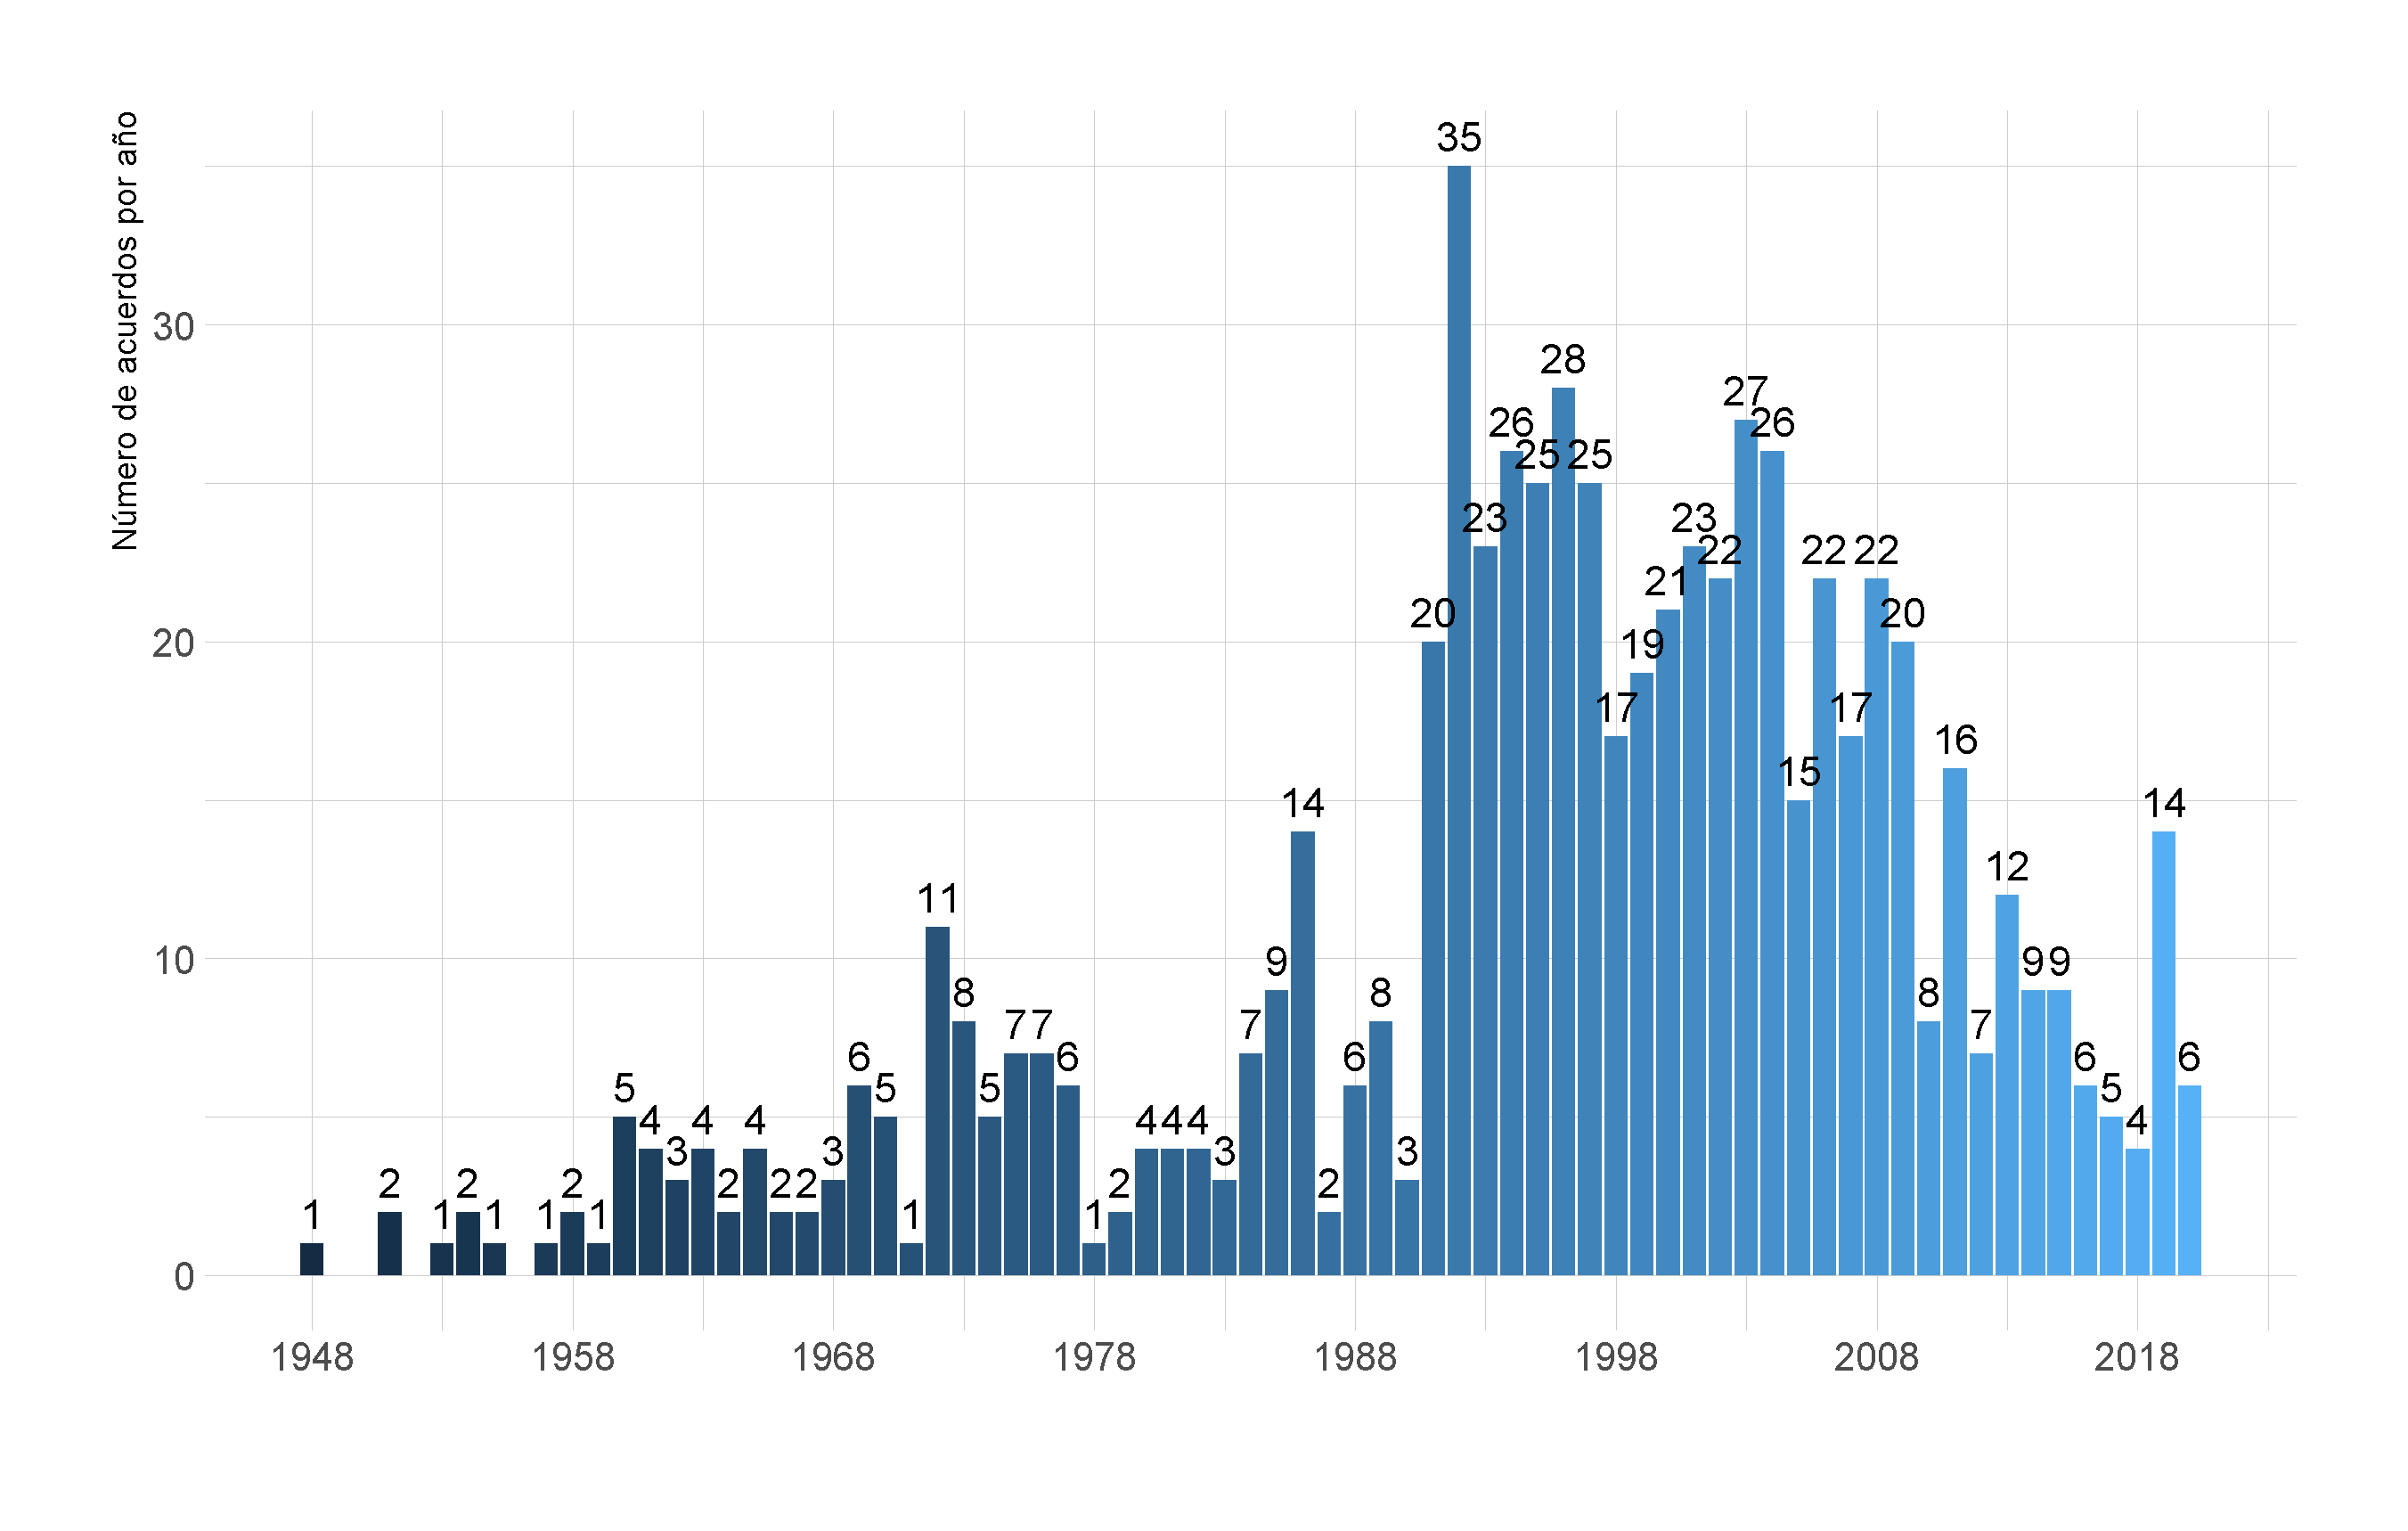
\includegraphics[width=.95\linewidth]{../01.Figures/figura_1}
  \\ \smallskip\noindent\scriptsize Fuente: Elaboración propia con base en DESTA (2022).
\end{marginfigure}

\justify{Los acuerdos comerciales no suelen ser considerados como un objeto de estudio, salvo algunas excepciones como en publicaciones de organismos internacionales (WTO, 2011; véase también Ravenhill, 2011) o aplicados a una región en particular, sin considerar su conjunto, con énfasis en la cantidad de acuerdos más que en el nivel de profundidad de los mismos (Cuevas, 2019).  Por el contrario, el papel del comercio, en general, es visto más bien desde el rol que tienen los flujos, como las exportaciones e importaciones de bienes y servicios, en la disminución de una probabilidad de conflicto (Baldwin, 1980; Bliss y Russett, 1998; McMillan, 1997). La mayor interdependencia que produce un mayor nivel de intercambio comercial debería aumentar cuando las partes involucradas son países democráticos (Gartzke, 2007; Liu y Ornelas, 2014; Polacheck, 1997; Ruggie, 1982). Esto se reflejaría en la profundidad de los compromisos adoptados en el proceso de negociación (Jo y Namgung, 2012).}

\justify{En relación con características institucionales que favorecerían acuerdos de libre comercio, en general se asume que un sistema democrático permite condiciones en que los acuerdos despliegan más abierta y eficientemente con respecto a la acción de grupos de interés. En regímenes democráticos existen mayores incentivos para cooperar y alcanzar e implementar acuerdos (Giuliano et al., 2010; Mansfield y Milner, 2012; Mansfield et al., 2002; Putnam, 1988). Adicionalmente, una mayor apertura comercial generaría una disminución del espacio de discrecionalidad que tendría una dictadura en su relación con grupos de interés, especialmente empresariales, por la reducción  que implicaría, por medio de la liberalización del comercio, del uso de subsidios o aranceles específicos, aun cuando hay evidencia reciente que indica una dirección contraria, en cuanto a que una mayor vinculación comercial fortalecería a un régimen dictatorial (Chang y Wen-Chin, 2016).}

\justify{Una segunda línea de argumentación asociada con una mayor profundidad que alcanza un acuerdo de libre comercio tiene que relación con la presencia de determinados capítulos, como los relativos a propiedad intelectual o inversiones (Morin y Suerbeck, 2020). Asimismo, existe un posible efecto inverso de cláusulas laborales, aun cuando esos vínculos causales son relativizados, en el sentido que la presencia de este tipo de acápites no tiene mayor importancia en una variación en el nivel de profundidad alcanzado (Càrrere et al., 2022).}

\justify{Un tercer aspecto tendría relación con el papel que tienen otro tipo de acuerdos previos, los que eventualmente tendrían una incidencia en la mayor profundidad que alcanza un acuerdo de libre comercio. En esto se ha abordado mayormente el papel que adquieren los acuerdos con la Unión Europea (UE) o Estados Unidos (EE.UU.), aun cuando más recientemente se ha expandido la investigación al rol que cumplen las negociaciones a un nivel multilateral (Elsig y Klotz, 2021). En esa línea argumentativa, entre las variaciones en el análisis se encuentran el estudio de las particularidades de estas contrapartes, como, por ejemplo, su carácter supranacional (Smith, 2015), la capacidad de inspirar diseños instituciones por parte de terceras partes, como ocurre con la propia UE como modelo de referencia (Lenz, 2012, 2021), o cuanto contrapartes de este tipo tienen la capacidad de movilizar intereses a favor o en contra de la suscripción de ese tipo de acuerdo, lo que se da especialmente en EE.UU. (Cuevas y Morillo-Remesnitzky, 2020; von Bülow, 2009).  Otro factor es el grado de homogeneidad en los recursos institucionales disponibles por las respectivas partes negociadoras, que son indicios en la variabilidad de asimetrías existentes (Hulse, 2017). No obstante, la influencia que eventualmente pueden tener tratados previos sobre la profundidad alcanzada ha sido relativizada, dado que el contenido de determinados capítulos tiende a replicar una proporción relevante del contenido de acuerdos de libre comercio preexistentes (56\%), alcanzando en el caso de los capítulos de Propiedad Intelectual e Inversiones un 72 y 65\%, respectivamente (Alle y Elsig, 2019).}

\justify{Una cuarta línea de argumentación tiene relación con las condicionantes de política doméstica en la variación del nivel de profundidad que alcanzan los acuerdos de libre comercio (Mansfield y Milner, 2012). En su canalización cumplen un papel preponderante los grupos de interés, ya sea para fortalecer la posición negociadora de un gobierno, a través de su apoyo, de canalizar dentro del espacio de negociación las críticas o de influir en las negociaciones (Anderer et al., 2020; Bull, 2008; Díez-Medrano, 2018; Dür y De Briève, 2007; Lechner, 2016; Mansfield y Milner, 2012; Putnam, 1988).}

\justify{Tomando en consideración los argumentos expuestos, la presencia de un mayor nivel democrático entre las partes concurrentes en un acuerdo de libre comercio aparecería como una variable que tendría un mayor efecto en el aumento del nivel de profundidad que toma un tratado, tanto porque permitiría mayores espacios para la inclusión de grupos de interés y con esto la diversificación de una agenda de negociadora que implique mayores grados de complejidad y profundidad en los compromisos que se pueden adoptar. Al mismo tiempo, los mayores niveles de democracia aparecerían también como potenciales variables explicativas por una cuestión reputacional del país, en que mayores concesiones son posibles precisamente como una suerte de incentivo por el tipo de políticas posibles de implementar en democracia, entre las que se incluyen medidas de globalización económica.}

\justify{Por lo tanto, la hipótesis que se plantea en el artículo es que una mayor profundidad de un acuerdo de libre comercio se explica esencialmente por el aumento del nivel democrático presente entre las partes que concurren en el acuerdo, siendo una variable más importante que la presencia de capítulos específicos o de contrapartes que plantean mayores exigencias como la UE. Al mismo tiempo, es una variable que refleja tanto la primera como cuarta de las condiciones planteadas previamente.}

\justify{En el caso de la presencia de capítulos específicos, se considera la presencia en un acuerdo de las secciones relativas a la propiedad intelectual e inversiones, las que darían cuenta del efecto que tendrían capítulos que buscan precisamente una mayor liberalización, al contener compromisos que involucran cambios regulatorios de mayor complejidad que medidas de reducción arancelaria (Chaisse, 2012; Frankel, 2012). En el caso de la diferenciación de acuerdos en los que está presente la UE, ello daría cuenta sí estos tratados efectivamente son impulsores de una mayor profundidad en los compromisos adquiridos. Ambas variables son incluidas como un posible control del efecto que toma un mayor nivel de democracia, dando con ella cuenta del segundo y tercer grupo de argumentos planteados.}

\justify{En el estudio se incorpora una cuarta variable para evaluar el posible efecto que tendría el período en el cual se firmó el acuerdo. En este caso en particular, su inclusión como un control se debe a que precisamente es entre las décadas de 19990 y 2000, en que se da mayoritariamente la firma de acuerdos de libre comercio (WTO, 2011), como se ve en reflejado en la Figura 1. Para esto, se definieron períodos basados en décadas, excepto en el caso del primer período (1948-1960) que fue de doce años.}

%%%%%%%%%%%%%%%%%%%%%%%%%%%%%%%%%%%%%%%%%%%%%%%%%%

\section[M\'etodo] {{\normalfont M\'etodo}}

%%%%%%%%%%%%%%%%%%%%%%%%%%%%%%%%%%%%%%%%%%%%%%%%%%

\subsection[Datos y medición] {Datos y medición}

\justify{En términos formales, el modelo que refleja las variables consideradas y su respectiva posición en términos de inclusión en la investigación se expresa de la siguiente forma:}

\begin{fullwidth}
\begin{equation}
Y_{Profundidad}= \beta_{0} + \beta_{Democracia}+ \beta_{Inversiones}+ \beta_{P. Intelectual}+\beta_{UE}+ \ \beta_{Periodo}+ \epsilon
\end{equation}
\end{fullwidth}

\justify{Posteriormente, se exponen los resultados a partir de la estimación de modelos de regresión lineal, presentados de manera secuencial (Harrel, 2001), donde se analiza qué ocurre con el efecto que toma la democracia sobre la profundidad de acuerdos comerciales, a medida que se agregan las respectivas variables de control. Finalmente, a partir de los resultados del último modelo y del análisis del cumplimiento de sus respectivos supuestos obtenidos, se analiza el efecto de los controles como posibles efectos de intermediación (Jaccard y Turrisi, 2003) o de grupo, por medio de efectos aleatorios (Gelman y Hill, 2017).}

\justify{La variable dependiente es la profundidad de un acuerdo de libre comercio, reflejado en el Índice de Profundidad de DESTA obtenido de una estimación de rasgos latentes con el modelo Rasch\footnote{Corresponde a un tipo de análisis aplicado originalmente en estudios psicométricos en los que se estima el esfuerzo requerido para responder correctamente un ítem (Bartolucci et al., 2016; Raykov y Marcoulides, 2018). En este caso se interpreta como el alcance que tienen los acuerdos comerciales analizados a partir del estudio del contenido de sus capítulos.}. Este resultado se expresa en una función logística, representada en un parámetro $\theta$, con un rango que oscila entre un mínimo de -1,50 y un máximo de 2,09, con un promedio de 0,07 y una desviación estándar de 1,04 puntos, en el cual un mayor número indica el mayor esfuerzo requerido, que en este artículo representa la profundidad que adquiere un acuerdo comercial. Para efectos de una interpretación más intuitiva de los resultados, la variable dependiente se presentó porcentualmente como la probabilidad obtenida a partir de exponenciar el parámetro $\theta$.}

\justify{El nivel democrático presente en un acuerdo se estimó a partir del promedio anual del índice liberal democracia liberal que tenía cada una de las partes involucradas en el año en que se firmó\footnote{En el caso que una de las partes fuese un grupo de países ({\itshape e.g.}, la Unión Europea), se empleó la misma medida de tendencia central. Cuando la unidad de observación correspondió a un conjunto de países ({\itshape e.g.}, MERCOSUR), el promedio fue la distancia entre los valores mínimo y máximo.}. Esta información fue obtenida de Varieties of Democracy (V-Dem; véase Coppedge et al., 2022). El efecto esperado es que un mayor nivel democracia incide en un incremento en la profundidad en los compromisos adquiridos en un acuerdo comercial.}
 
\justify{Los resultados en general muestran que el nivel promedio es de 48,18 puntos, lo que indica que las partes concurrentes en un acuerdo comercial son países medianamente democráticos. Si bien el rango es bastante amplio, 4,25 y 85,20 puntos respectivamente, lo que refleja acuerdos con contrapartes poco o nada o muy democráticas, la medianía en términos democráticos es lo que mejor refleja esta variable, al ser la mediana muy similar al promedio (49) y a una variabilidad de 21,39 puntos, equivalente en a un 44,40\% si consideramos su coeficiente de varianza, como se ve en la Tabla 1, siendo la relación entre ambas variables medianamente estrecha como se ve en la Figura 2.}

\begin{marginfigure}
  \centering
  \smallskip\noindent\small Figura 2 \\ Relación entre profundidad de acuerdos y democracia
  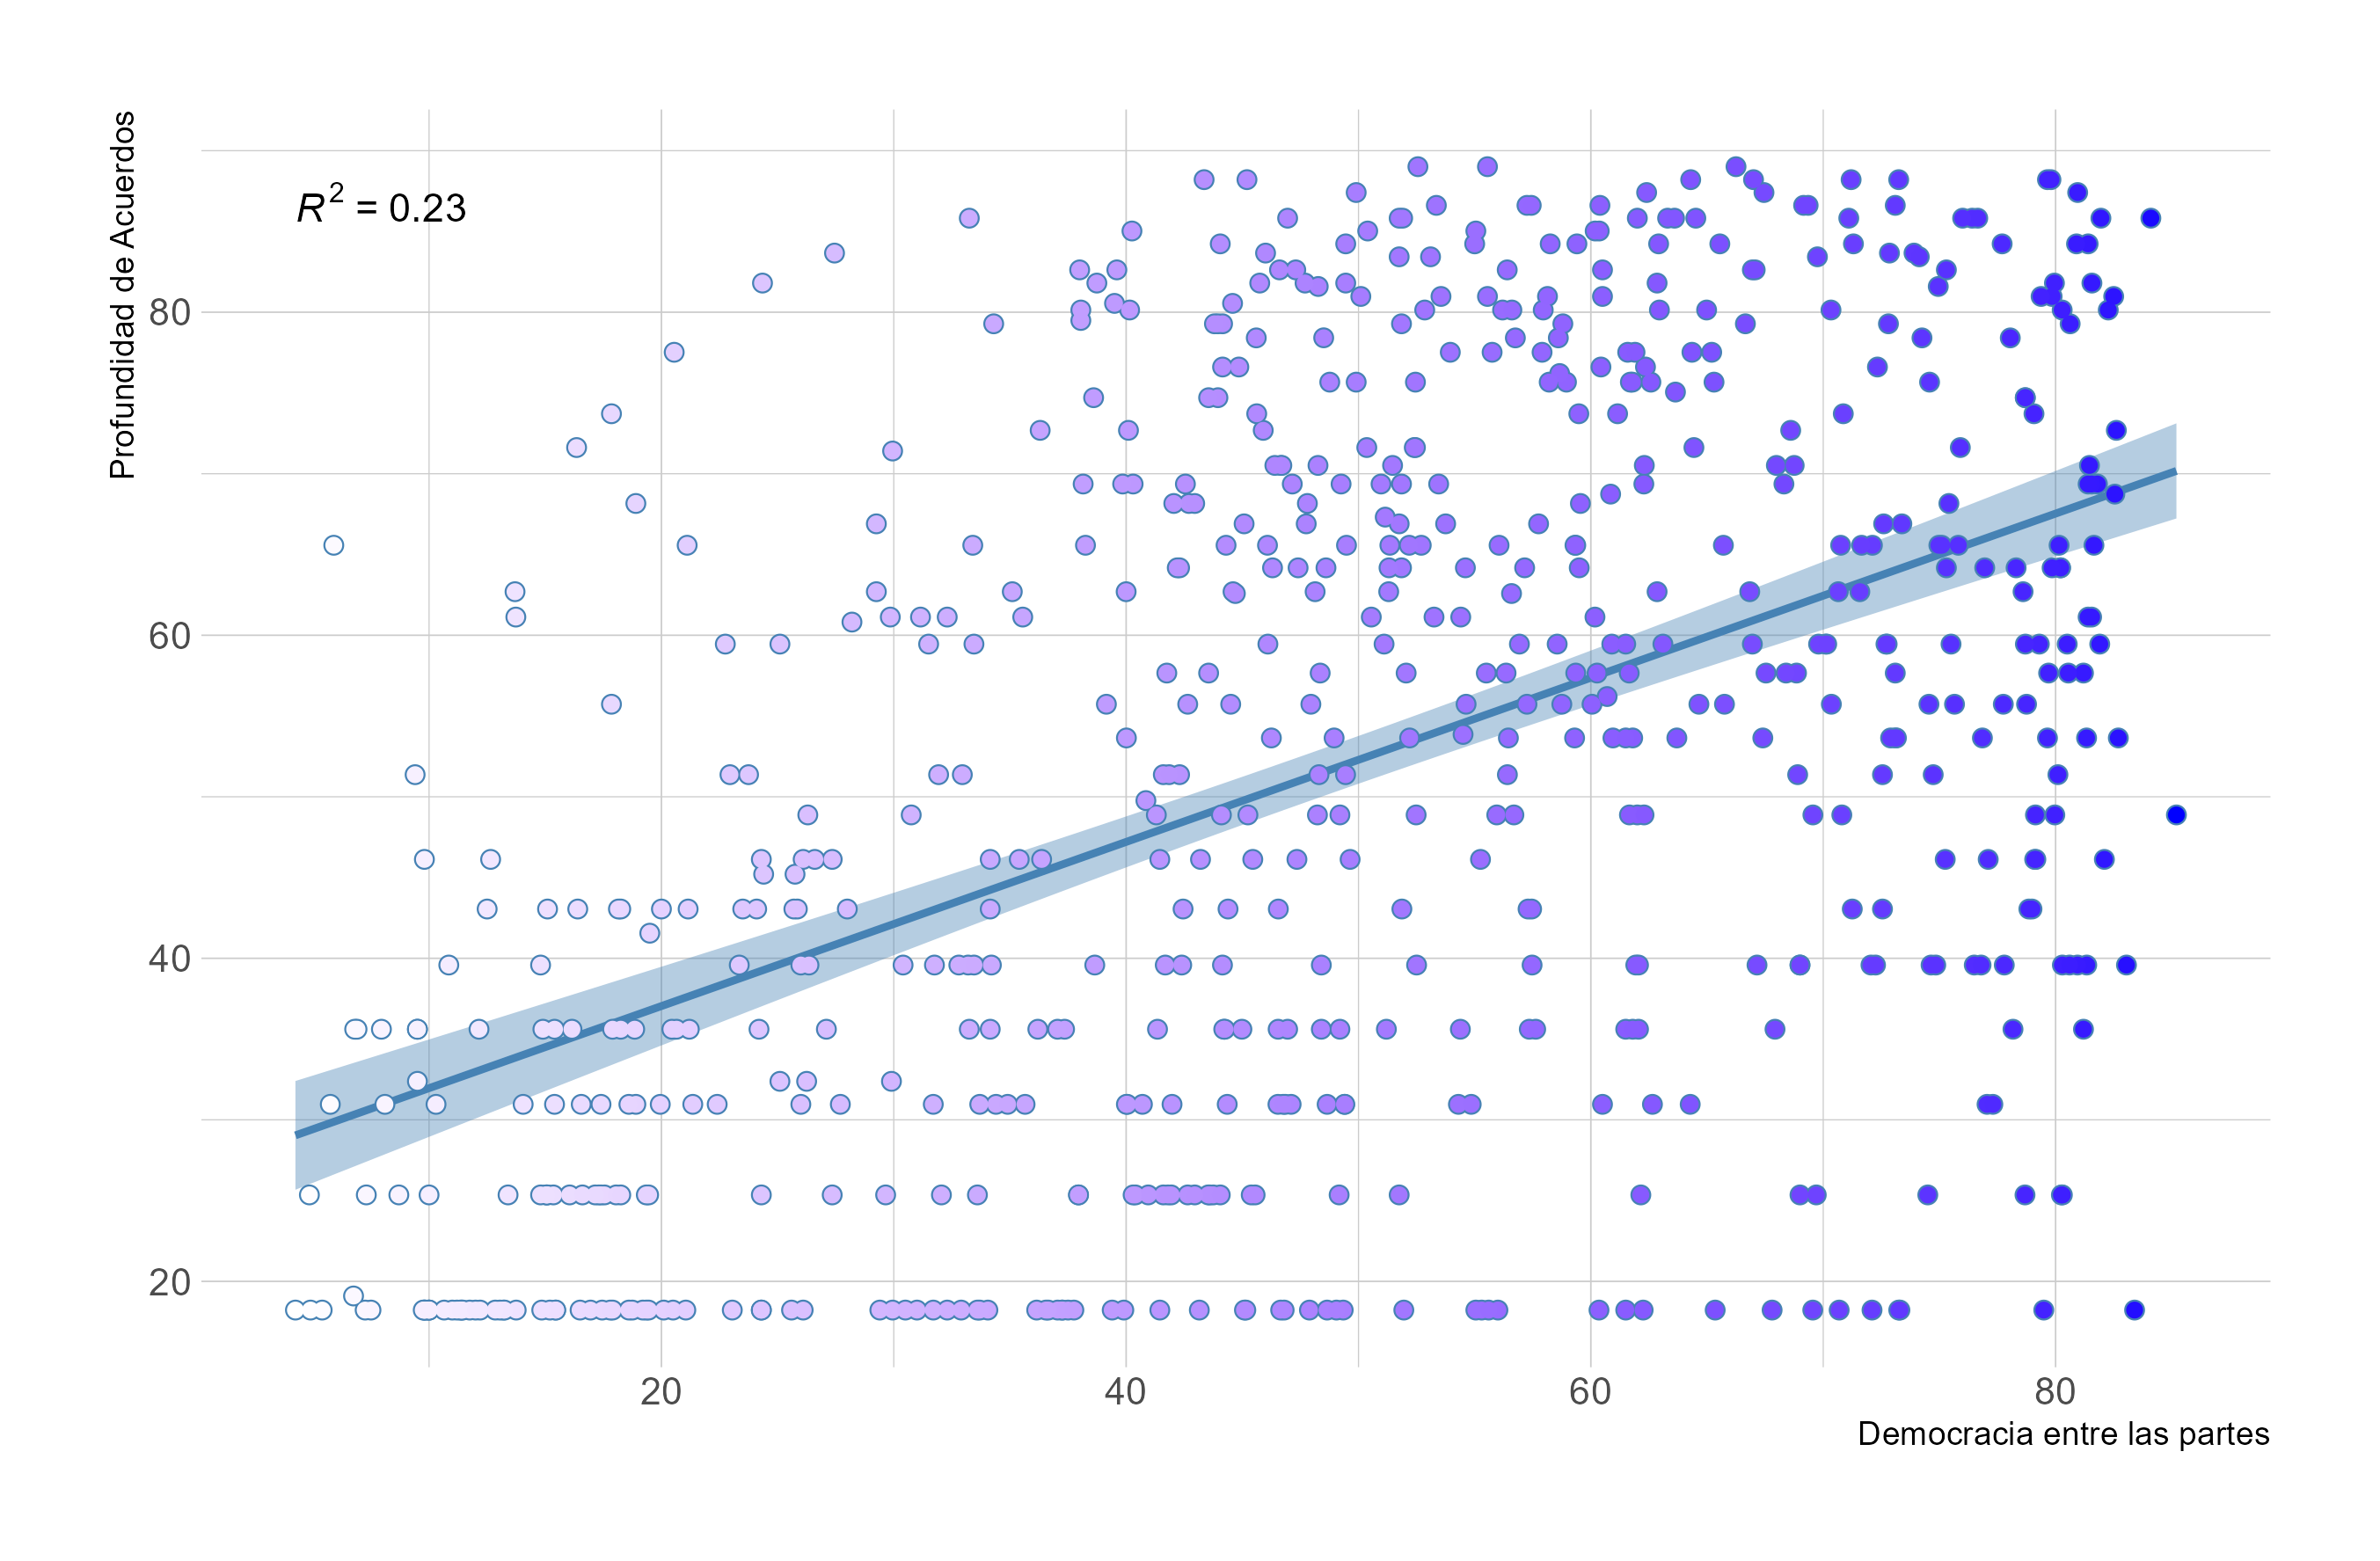
\includegraphics[width=.95\linewidth]{../01.Figures/figura_2}
  \\ \smallskip\noindent\scriptsize Fuente: Elaboración propia con base en DESTA (2022) y Coppedge et al. (2022).
\end{marginfigure}

\justify{En el caso de la inclusión de la presencia de capítulos de Propiedad Intelectual e Inversiones (Chaisse, 2012; Frankel, 2012). Si bien ambas variables están bastante asociadas (V de Cramer = 0,546), en función de los antecedentes teóricos relativos a la inclusión de estos capítulos como potenciales predictores de la profundidad de acuerdos, se incluyen como posibles predictores. }

\justify{En aquellos acuerdos que tienen capítulos de propiedad intelectual ($n$ = 210) el promedio de profundidad es de 74,91, frente a 40,96 puntos entre aquellos casos en que no está presente ese acápite ($n$ = 482). Esta diferencia de 33,95 es confirmada a un 99,99\% ($p \leq 0,000$ de prueba de Tukey). En el caso de los tratados en que hay compromisos en materia de protección de inversiones, el promedio de profundidad es de 71,90 y 33,93 puntos de diferencia, frente a un 37,97 en caso de aquellos acuerdos con que no lo tienen (Figura 3), confirmadas a un 99,99\%.}

\justify{Al considerar las diferencias según periodo, entre 1981 y 1990 es cuando el nivel de profundidad fue menor, con un 25,67, mientras que el período entre 2010 y 2020 alcanza 74,44 puntos. A partir de 1990 comienzan a verse mayores niveles de profundidad, lo que va en línea respecto a ubicar en esa década cuando el fenómeno de los acuerdos de libre comercio se generaliza (Figura 1) (WTO, 2011). La mayor diferencia se da entre lo que ocurre entre las décadas de 2010 (período 2011/2020) y 1980 (1981-1990), con 48,76 puntos (Figura 3). La mayor cantidad de acuerdos se da en la década de 2000.}

\justify{Finalmente, un cuarto tipo de control es si la presencia de la UE como contraparte incrementa (o no) sus niveles de profundización, al ser instrumentos de promoción de sus valores en materias como la democracia y promoción de derechos humanos (Velluti, 2020). La profundidad de los acuerdos de la UE es de un 57,24 frente a un 50,37(Figura 3). La diferencia de 6,87 es confirmada a un 99,9\% de confianza (Prueba Tukey).}

\begin{table*}[h]
  \centering
  \fontfamily{ppl}\selectfont
   \smallskip\noindent\small Tabla 1 \\ Operacionalización de variable independiente y dependientes \\~\\
  \begin{tabular}{c c c c c c c}
    \toprule
    Tipo & Variable & Promedio & Desvío estándar & Min. & Máx. & Fuente \\
    \midrule
    \multirow{3}{*}{Dependiente} & Rasch Index & 0,07 & 1,04 & $-$1,50 & 2,09 & \multirow{3}{*}{DESTA} \\ 
     & Profundidad & \multirow{2}{*}{51,26} & \multirow{2}{*}{22,41} & \multirow{2}{*}{18,22} & \multirow{2}{*}{89,01} & \\ 
     & de Acuerdos (\%) & & & & & \\ \midrule
    \multirow{2}{*}{Independiente} & Nivel de democracia & \multirow{2}{*}{48,2} & \multirow{2}{*}{21,4} & \multirow{2}{*}{4,25} & \multirow{2}{*}{85,2} & \multirow{2}{*}{V-Dem} \\
    & de las partes & & & & & \\ \midrule
    & & Frecuencia	& Porcentaje & & & \\ \midrule
    \multirow{2}{*}{Control} & \multirow{2}{*}{Capítulo de Inversiones} & Sí = 217 & Sí = 39,16 & \multirow{2}{*}{0} & \multirow{2}{*}{1} & \multirow{2}{*}{DESTA} \\ 
    & & No = 421 & No = 60,84 & & & \\ \midrule
    \multirow{2}{*}{Control} & Capítulo de Propiedad & Sí = 210 & Sí = 30,35 & \multirow{2}{*}{0} & \multirow{2}{*}{1} & \multirow{2}{*}{DESTA} \\ 
    & Intelectual & No = 482 & No = 69,65 & & & \\ \midrule
    \multirow{7}{*}{Control} & \multirow{7}{*}{Período} & 1948--1960 = 16 & 1948--1960 = 2,31 & \multirow{7}{*}{1} & \multirow{7}{*}{7} & \multirow{7}{*}{DESTA} \\
    & & 1961--1970 = 35 & 1961--1970 = 5,06 & & & \\ 
    & & 1971--1980 = 52 & 1971--1980 = 7,51 & & & \\
    & & 1981--1990 = 60 & 1981--1990 = 8,67 & & & \\ 
    & & 1991--2000 = 239 & 1991--2000 = 34,54 & & & \\
    & & 2001--2010 = 202 & 2001--2010 = 29,19 & & & \\ 
    & & 2011--2020 = 88 & 2011--2020 = 12,72 & & & \\ \midrule
    \multirow{2}{*}{Control} & \multirow{2}{*}{Acuerdo con la UE} & Sí = 90 & Sí = 13 & \multirow{2}{*}{1} & \multirow{2}{*}{0} & \multirow{2}{*}{DESTA} \\
    & & No = 602 & No = 87 &  &  & \\ \bottomrule
  \end{tabular}
  \\~\\ \smallskip\noindent\scriptsize Fuente: Elaboración propia con base en DESTA (2022) y Coppedge et al. (2022).
\end{table*}

\begin{figure*}[h!]
\captionsetup[subfigure]{labelformat=empty}
  \centering
  \smallskip\noindent\small Figura 3 \\ Profundidad de acuerdos, según presencia de capítulo de propiedad intelectual, presencia capítulo de inversiones, período y presencia de acuerdo con la UE
  \subfloat[Cap. Propiedad Intelectual]{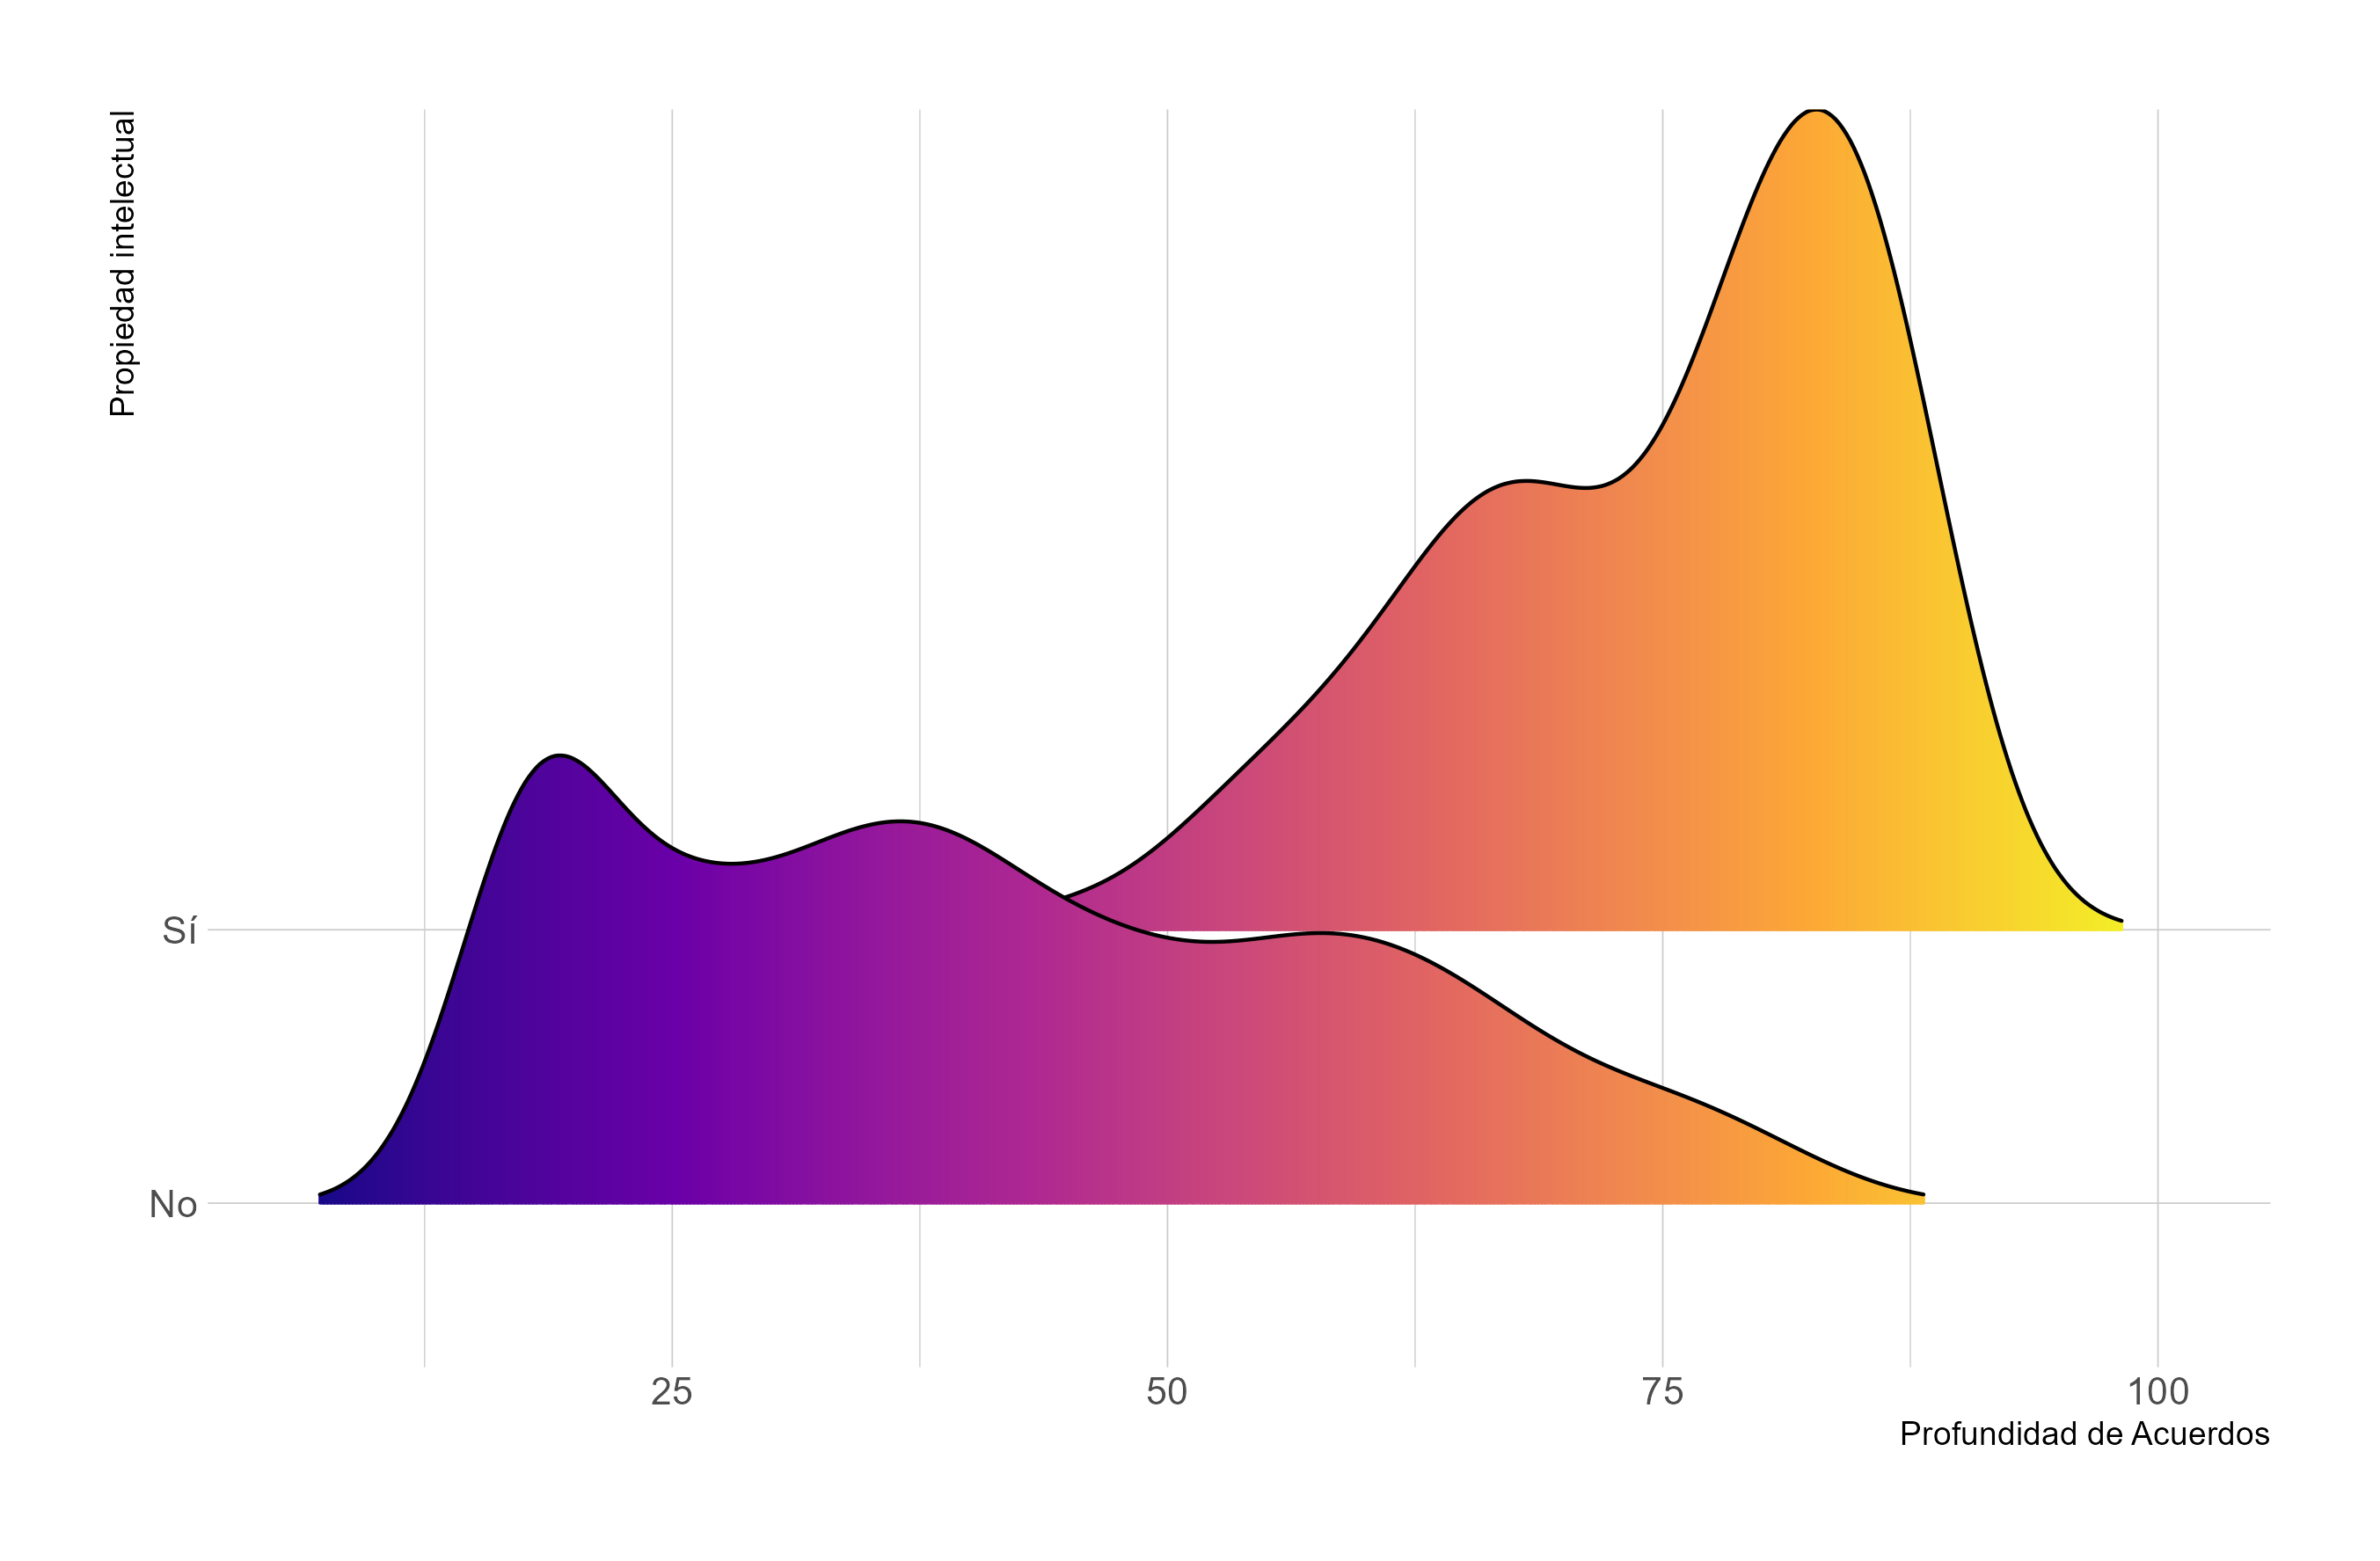
\includegraphics[width=.49\linewidth]{../01.Figures/figura_3a}}
  \subfloat[Cap. Inversiones]{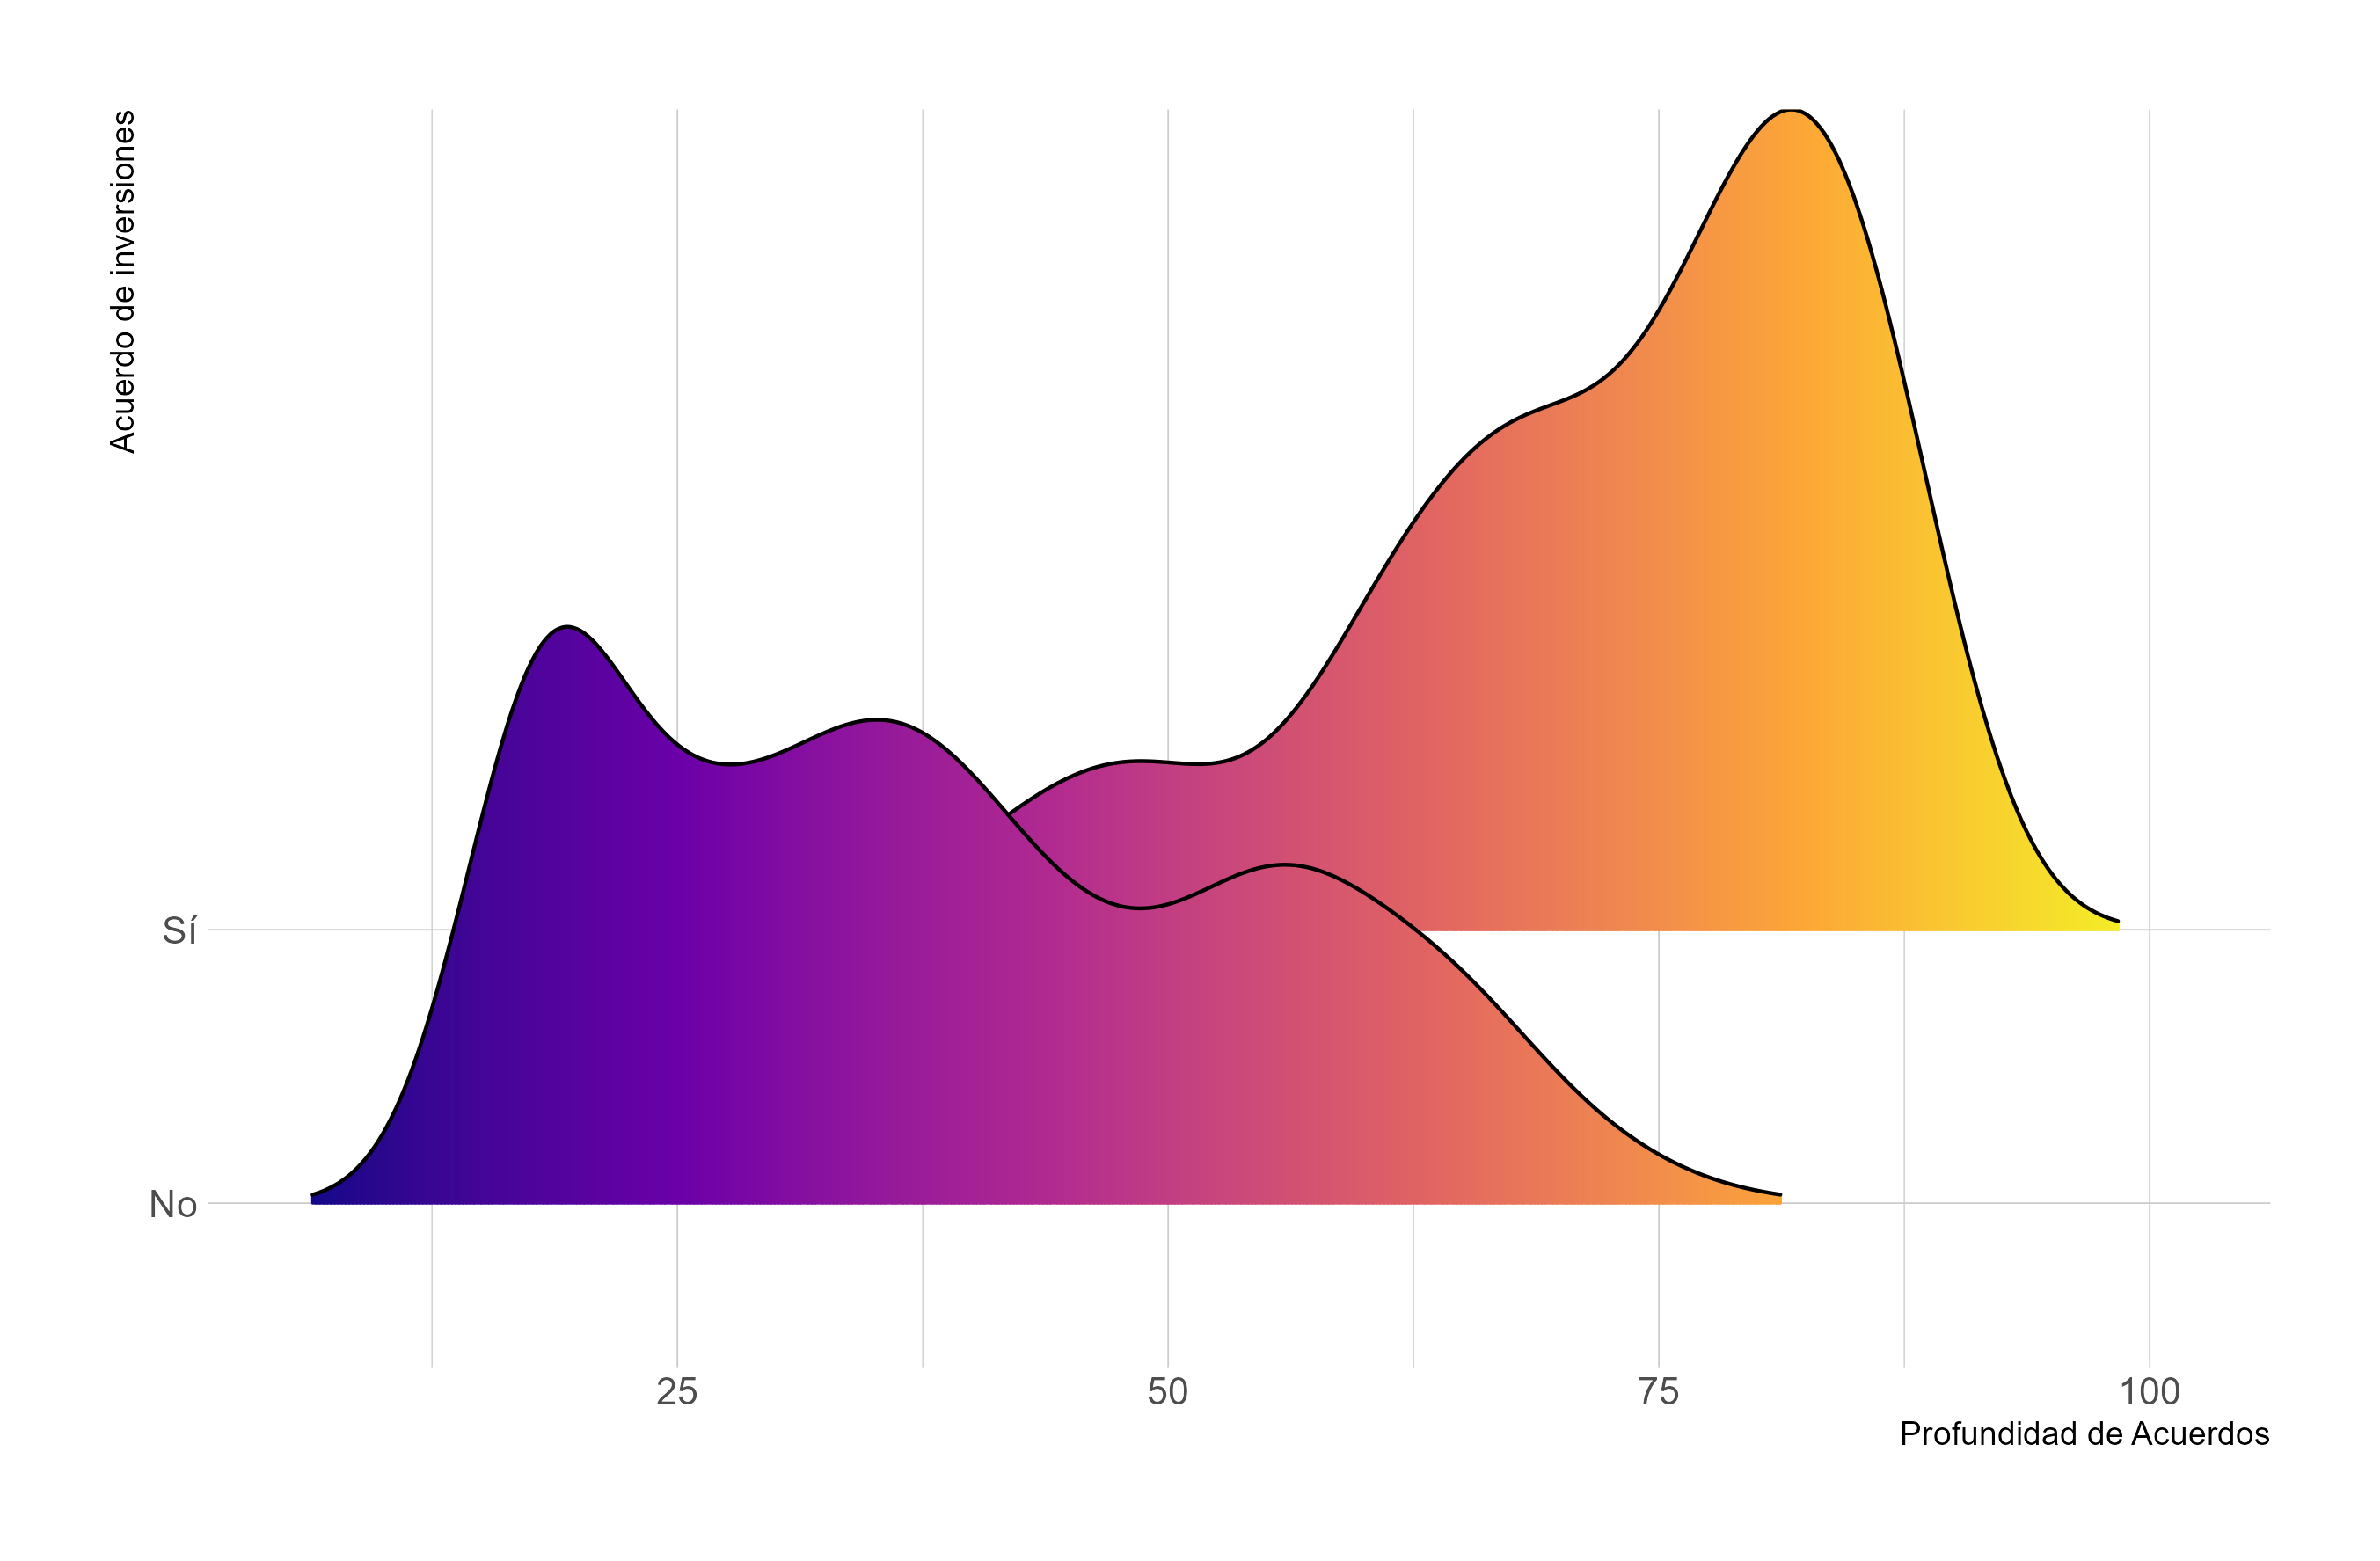
\includegraphics[width=.49\linewidth]{../01.Figures/figura_3b}}\\
   \subfloat[Período]{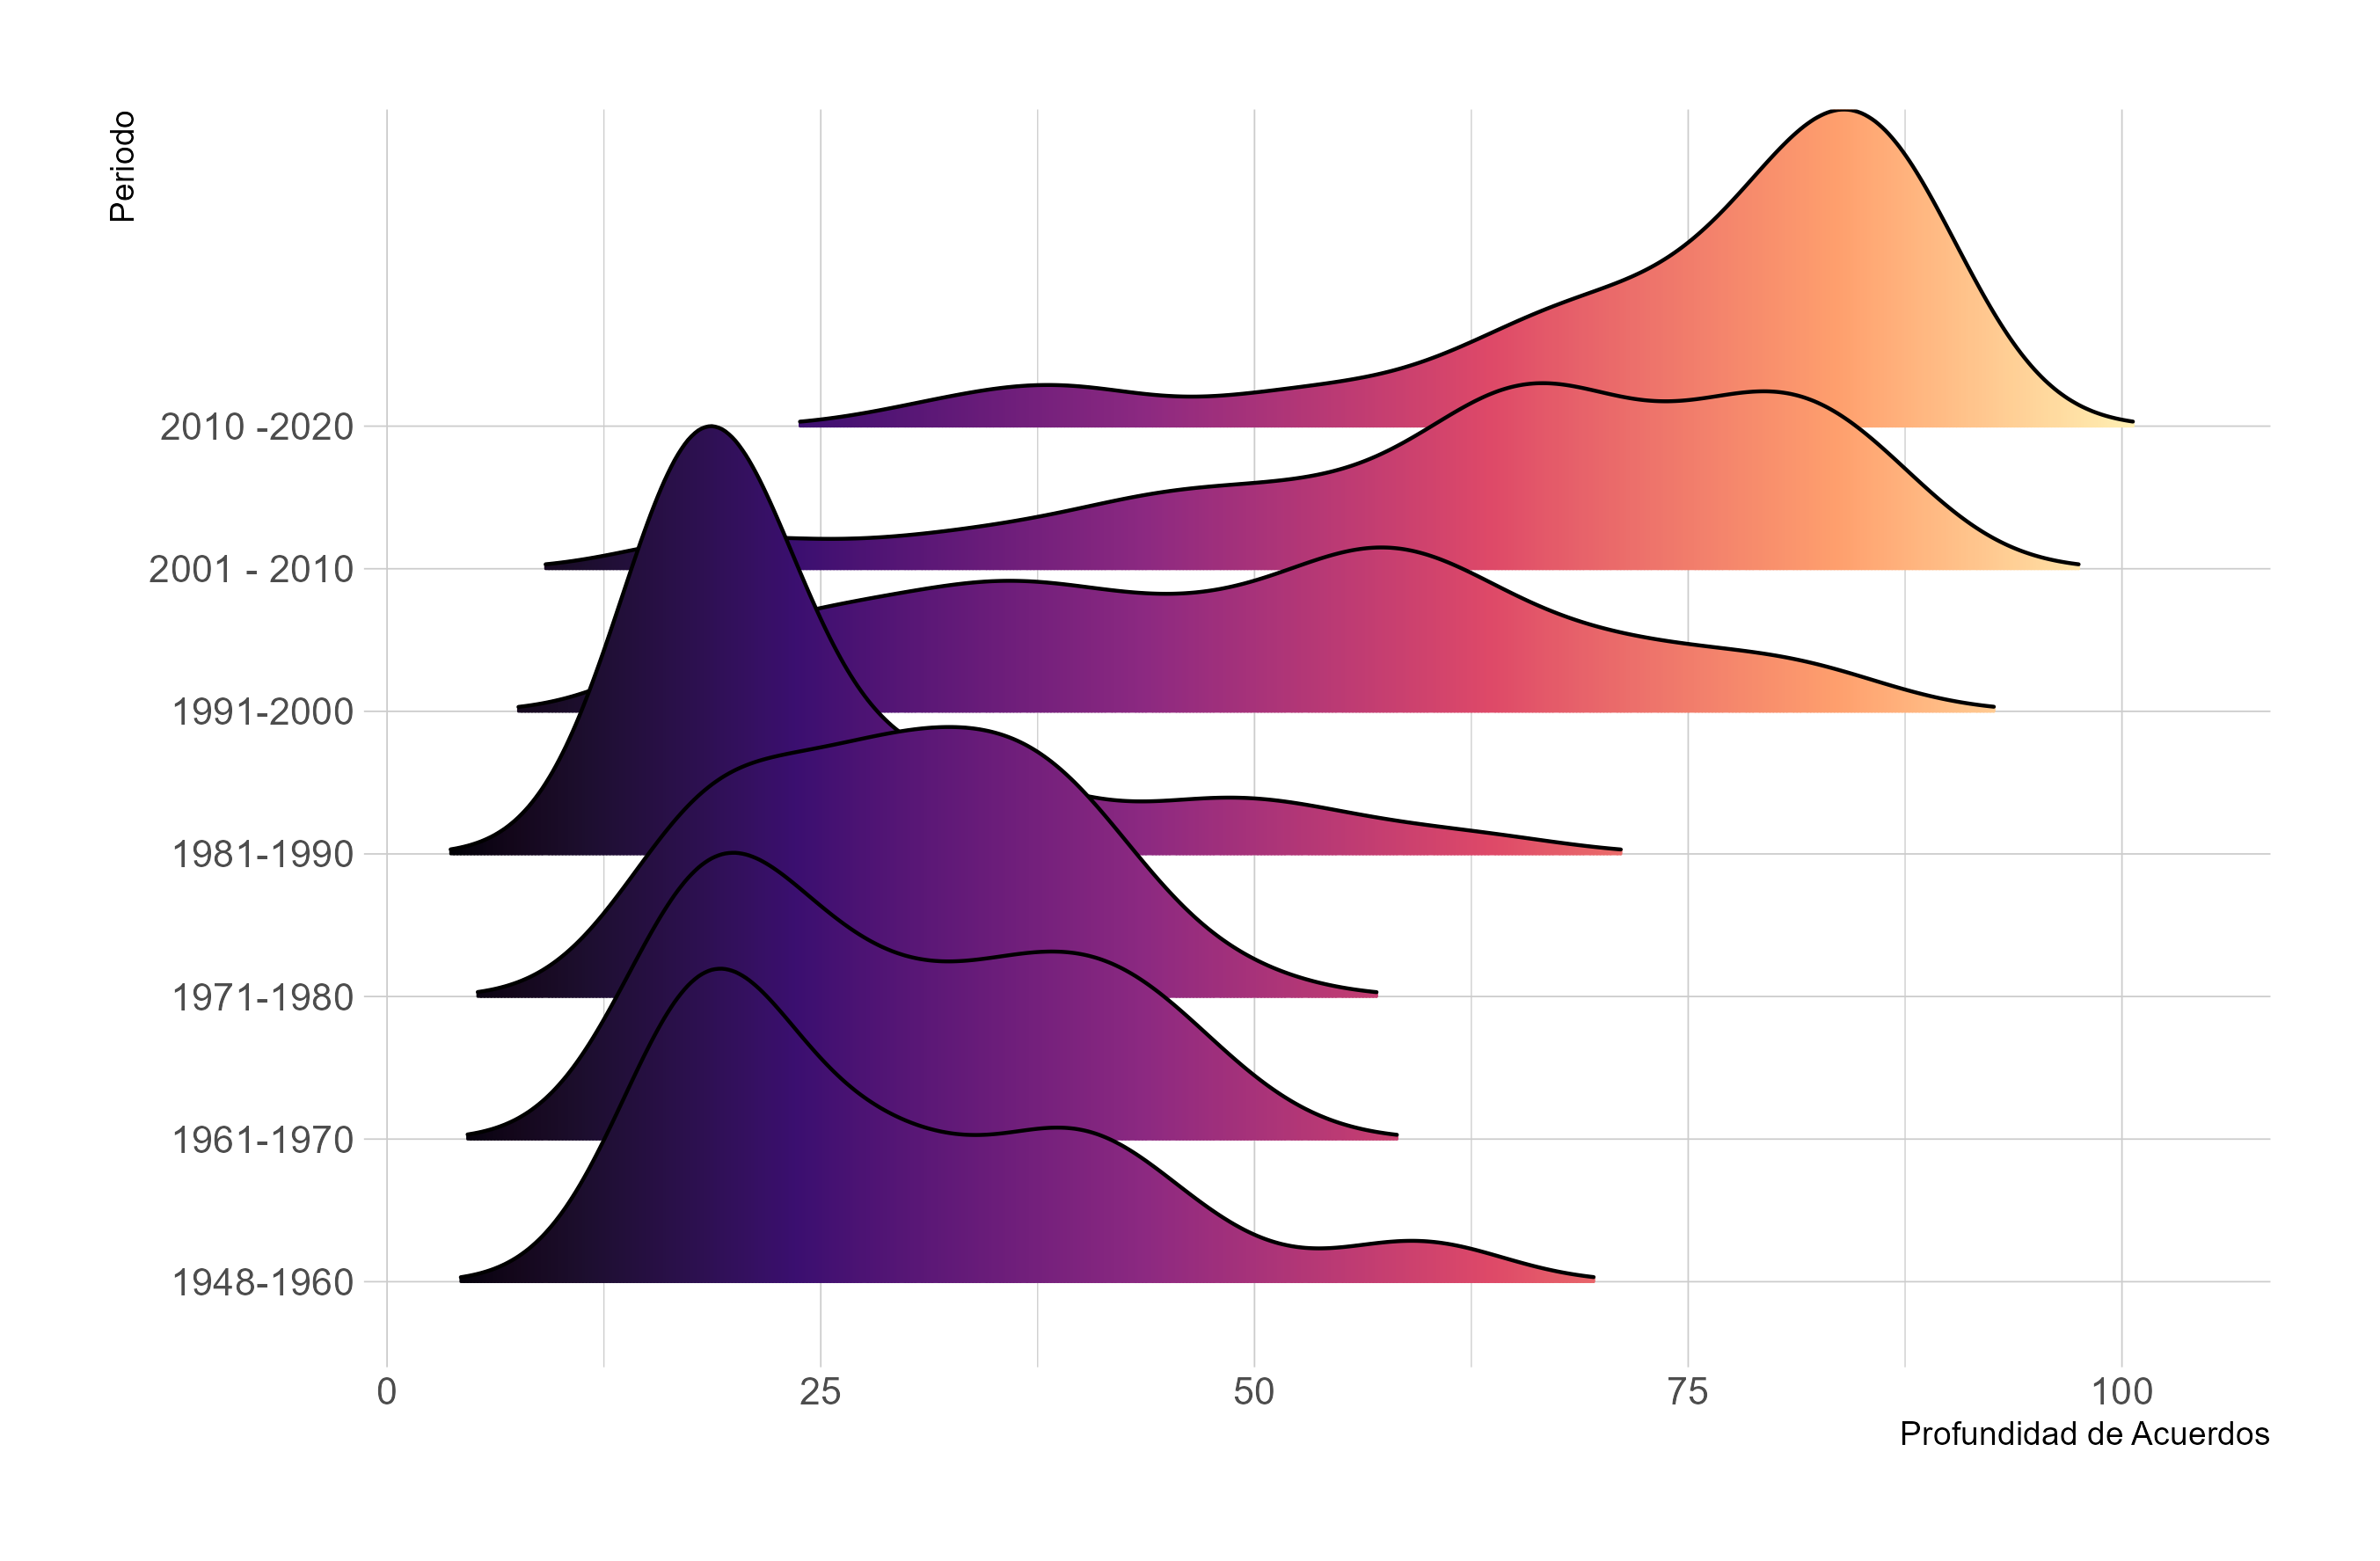
\includegraphics[width=.49\linewidth]{../01.Figures/figura_3c}}
   \subfloat[Acuerdo UE]{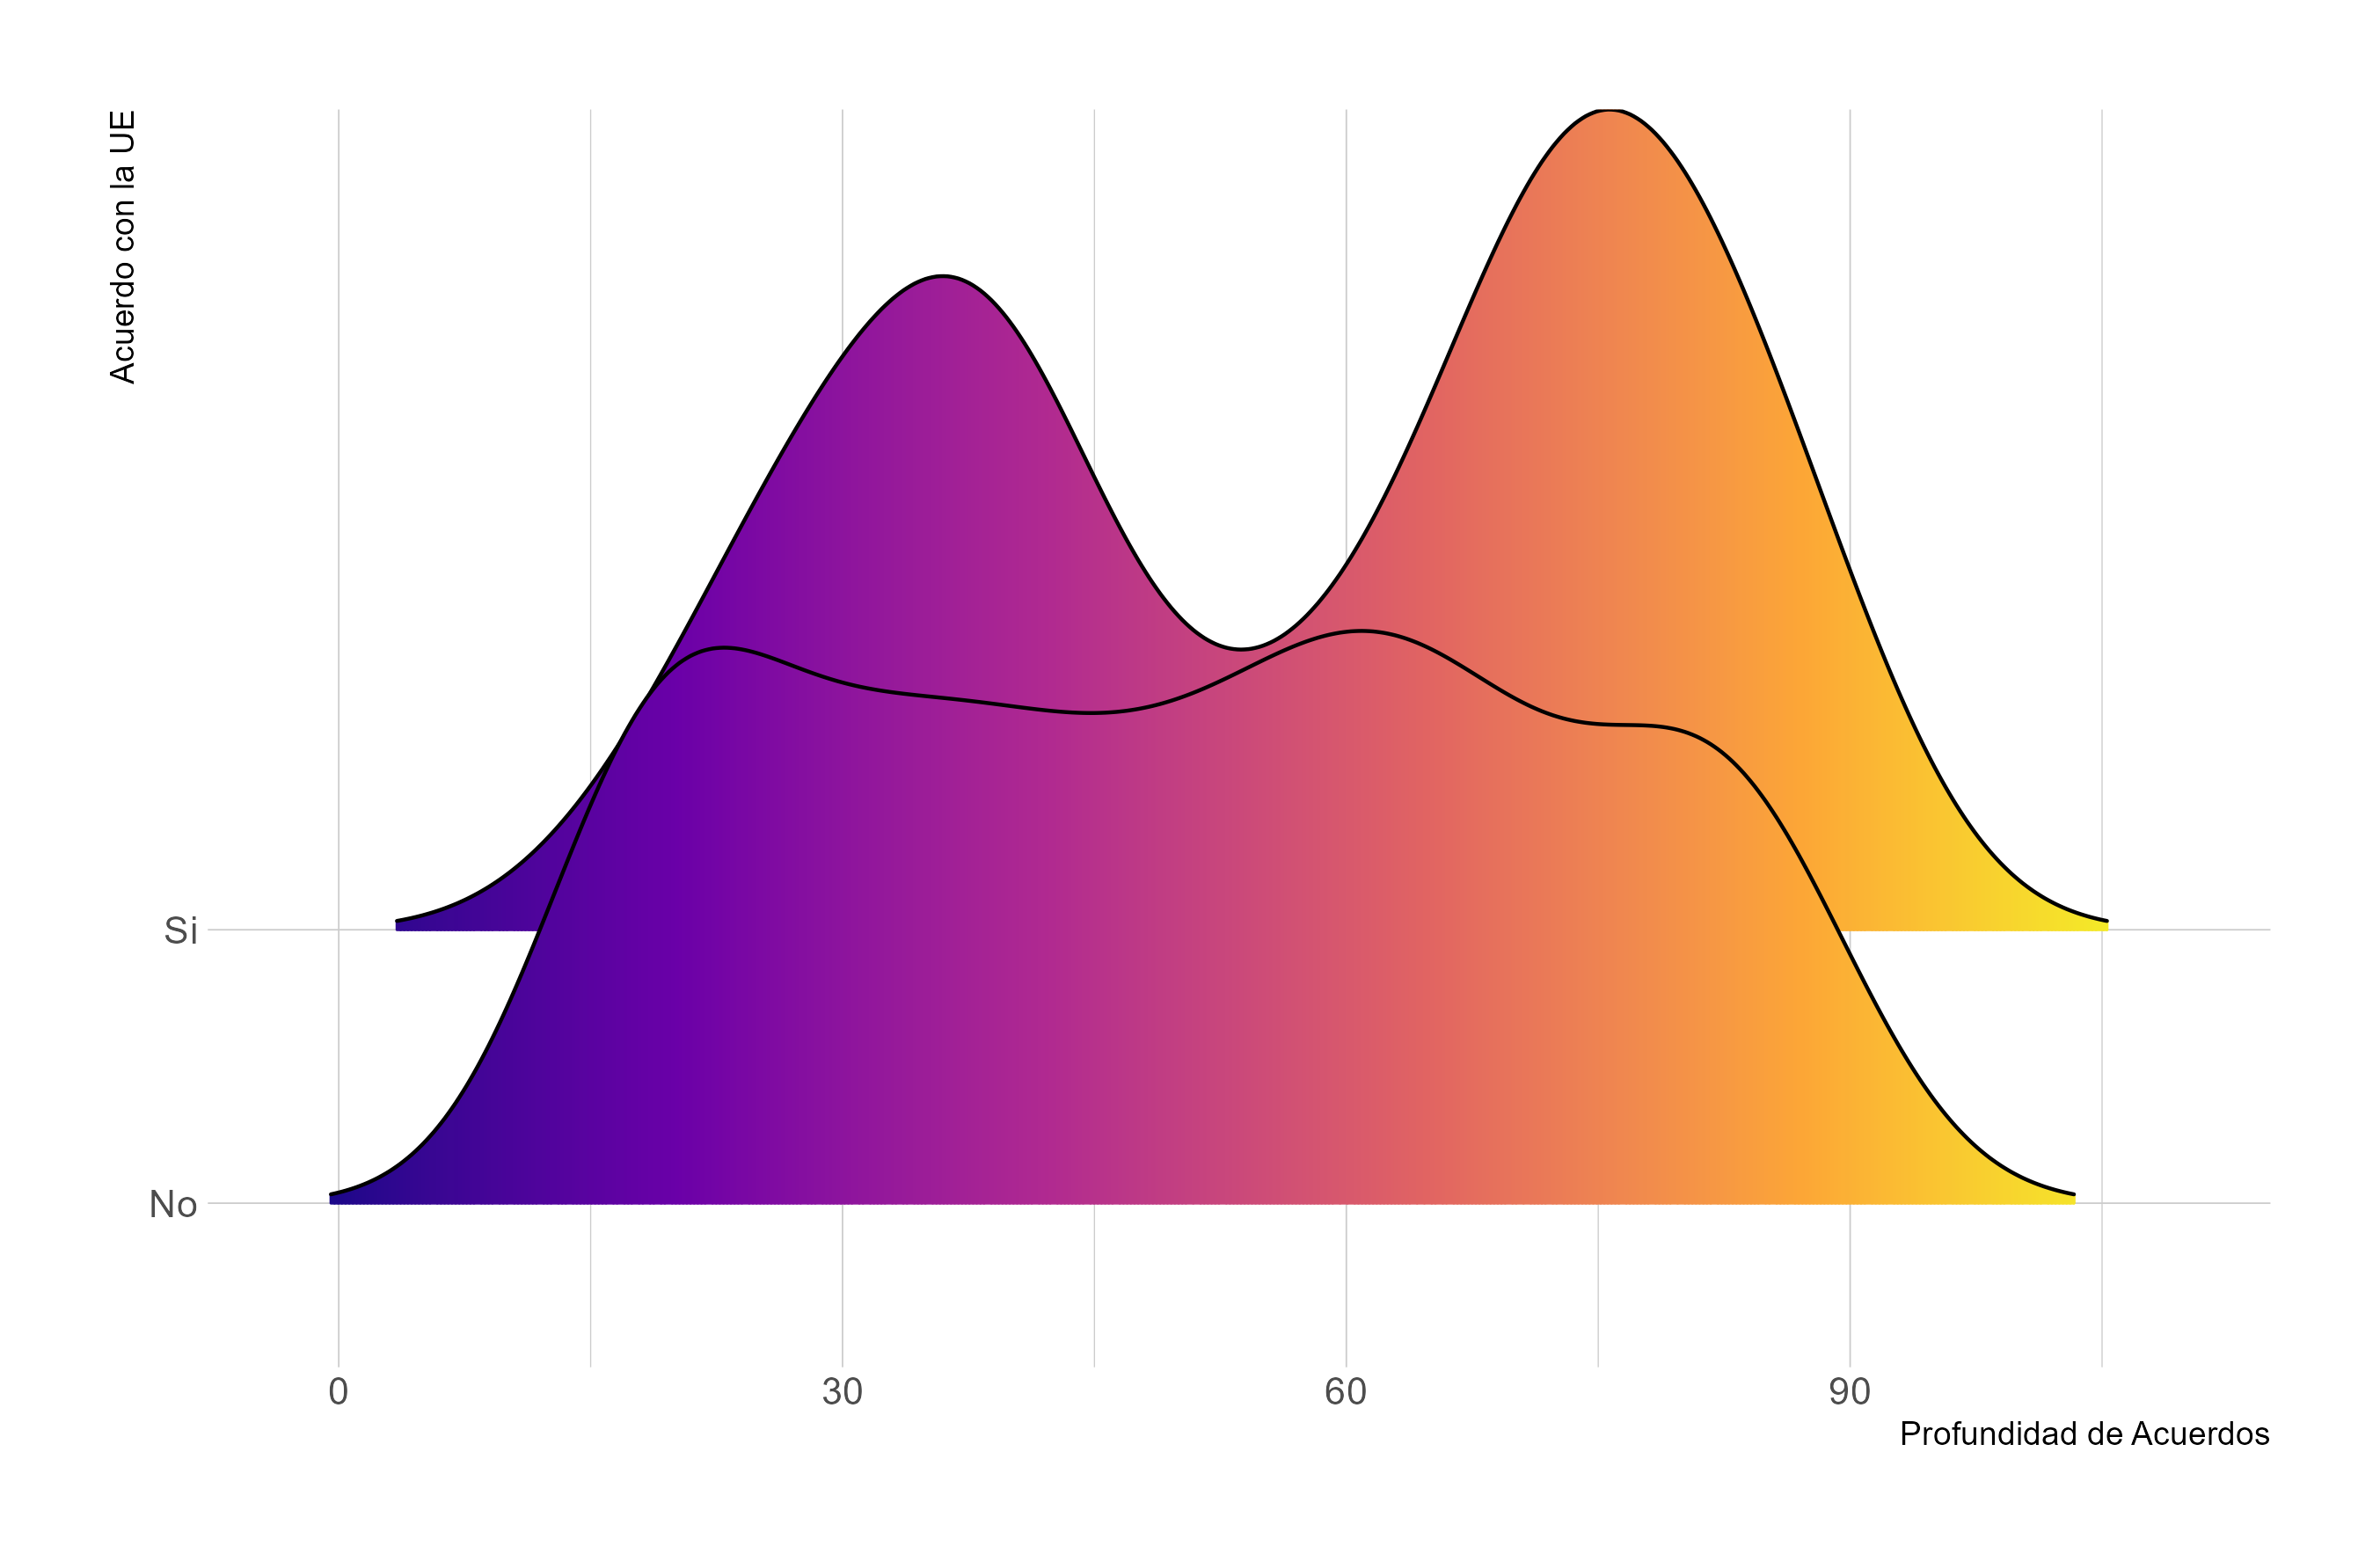
\includegraphics[width=.49\linewidth]{../01.Figures/figura_3d}}
  \\ \smallskip\noindent\scriptsize Fuente: Elaboración propia con base en DESTA (2022).
\end{figure*}

%%%%%%%%%%%%%%%%%%%%%%%%%%%%%%%%%%%%%%%%%%%%%%%%%%

\section[Resultados] {{\normalfont Resultados}}

%%%%%%%%%%%%%%%%%%%%%%%%%%%%%%%%%%%%%%%%%%%%%%%%%%

\justify{El efecto que toma el aumento cada punto del nivel democracia de las partes involucradas es de un incremento de 0,5 puntos en su nivel de profundización. Esto refleja en principio una importancia bastante relevante, considerando además que su bondad de ajuste es importante al ser solo una variable ($R^{2} = 0,235$). Este resultado se alinearía con que las partes que tienen un mayor nivel de democracia tienden a tener vínculos comerciales más profundos (Tabla 2).}

\justify{La presencia de un capítulo de inversiones tiene un efecto importante en el nivel de profundidad de un acuerdo, de 30 puntos más que cuando no está presente. Asimismo, su ajuste también aumenta de forma importante: a un $R^{2} = 0,632$. La presencia de un apartado de propiedad intelectual también es bastante importante, 18 puntos más que cuando no lo está. Su contribución al aumento de un $R^{2}$ también es de nueve puntos: $R^{2} = 0,721$. Al mismo tiempo, el impacto de un mayor nivel democrático tiende a decrecer de manera bastante acelerada cuando se incluyen estas dos variables (Tabla 2).}

\begin{table*}[h]
  \centering
  \fontfamily{ppl}\selectfont
   \smallskip\noindent\small Tabla 2 \\ Profundidad de acuerdos de libre comercio y democracia \\~\\
  \begin{tabular}{l c c c c c}
    \toprule
     & Modelo I & Modelo II & Modelo III & Modelo IV & Modelo V \\ \midrule
    \multirow{2}{*}{Nivel de democracia} & 0,508$^{\star\star\star}$ & 0,316$^{\star\star\star}$  & 0,25$^{\star\star\star}$  & 0,22$^{\star\star\star}$  & 0,20$^{\star\star\star}$ \\
    & {\scriptsize (0,035)} & {\scriptsize (0,025)} & {\scriptsize (0,02)} & {\scriptsize (0,02)} & {\scriptsize (0,02)} \\ 
    \multirow{2}{*}{Cap. Inversiones} & & 30,097$^{\star\star\star}$ & 21,828$^{\star\star\star}$ & 17,551$^{\star\star\star}$ & 17,285$^{\star\star\star}$ \\
    & & {\scriptsize (1,109)} & {\scriptsize (1,115)} & {\scriptsize (1,087)} & {\scriptsize (1,001)} \\
    \multirow{2}{*}{Cap. Prop. Intelectual} & & & 17,727$^{\star\star\star}$ & 13,137$^{\star\star\star}$ & 13,277$^{\star\star\star}$ \\
    & & & {\scriptsize (1,196)} & {\scriptsize (1,087)} & {\scriptsize (1.077)} \\
    \multirow{2}{*}{Período 1961--1970} & & & & 0,622  & 0,030 \\
    & & & & {\scriptsize (3,110)} & {\scriptsize (3,083)} \\
    \multirow{2}{*}{Período 1971--1980} & & & & 1,769 & 0,388 \\
    & & & & {\scriptsize (2,921)} & {\scriptsize (2,915)} \\
    \multirow{2}{*}{Período  1981--1990} & & & & -3,319 & -2,892 \\
    & & & & {\scriptsize (2,877)} & {\scriptsize (2,851)} \\
    \multirow{2}{*}{Período 1991--2000} & & & & 10,687$^{\star\star\star}$ & 11,043$^{\star\star\star}$ \\
    & & & & {\scriptsize (2,654)} & {\scriptsize (2,629)} \\ 
    \multirow{2}{*}{Período  2001--2010} & & & & 17,193$^{\star\star\star}$ & 17,802$^{\star\star\star}$ \\
    & & & & {\scriptsize (2,707)} & {\scriptsize (2,685)}\\ 
    \multirow{2}{*}{Período 2010--2020} & & & & 19,771$^{\star\star\star}$ & 20,239$^{\star\star\star}$ \\
    & & & & {\scriptsize (2,905)} & {\scriptsize (2,879)} \\
    \multirow{2}{*}{Acuerdo UE} & & & & & 4,807$^{\star\star\star}$ \\
    & & & & & {\scriptsize (1,258)}\\ \midrule
    \multirow{2}{*}{Constante} & 26,878$^{\star\star\star}$ & 24,245$^{\star\star\star}$ & 25,314$^{\star\star\star}$ & 18,717$^{\star\star\star}$ & 19,028$^{\star\star\star}$ \\
    & {\scriptsize (1,850)} & {\scriptsize (1,288)} & {\scriptsize (1,123)} & {\scriptsize (2,653)} & {\scriptsize (2,628)} \\ \midrule
    $N$ & 686 & 686 & 686 & 686 & 686 \\ \midrule
    $R^2$ & 0,235 & 0,632 & 0,721 & 0,796 & 0,800 \\
    Adj. $R^2$ & 0,234 & 0,631 & 0,720 & 0,793 & 0,797 \\ \bottomrule
  \end{tabular}
  \\~\\ \smallskip\noindent\scriptsize $\star$ $p \leq 0,05$ | $\star\star$ $p \leq 0,01$ | $\star\star\star$ $p \leq 0,001$  \\ Fuente: Estimación propia con base en DESTA (2022) y Coppedge et al. (2022)
\end{table*}

\justify{Al tomar en cuenta el período en el cuál estos fueron firmados, siendo el lustro de referencia (1948--1960), las diferencias son relevantes a partir de 1990, en especial la comparación con la década de los 2000 en adelante. Estos resultados muestran que efectivamente la década de 1990 es un punto de inflexión relevante. Finalmente, la presencia de un acuerdo con la UE, serían cerca de cuatro puntos más.  Esto indicaría que efectivamente un acuerdo con esta región tiende a incrementar el nivel de profundidad que un tiene un acuerdo de libre comercio. Al incorporar estas dos variables, el efecto que toma la democracia sobre el nivel de profundidad disminuye de manera significativa (Figura 4).}

\begin{figure*}[h!]
\captionsetup[subfigure]{labelformat=empty}
  \centering
  \smallskip\noindent\small Figura 4 \\ Democracia y profundidad de acuerdos
  \subfloat{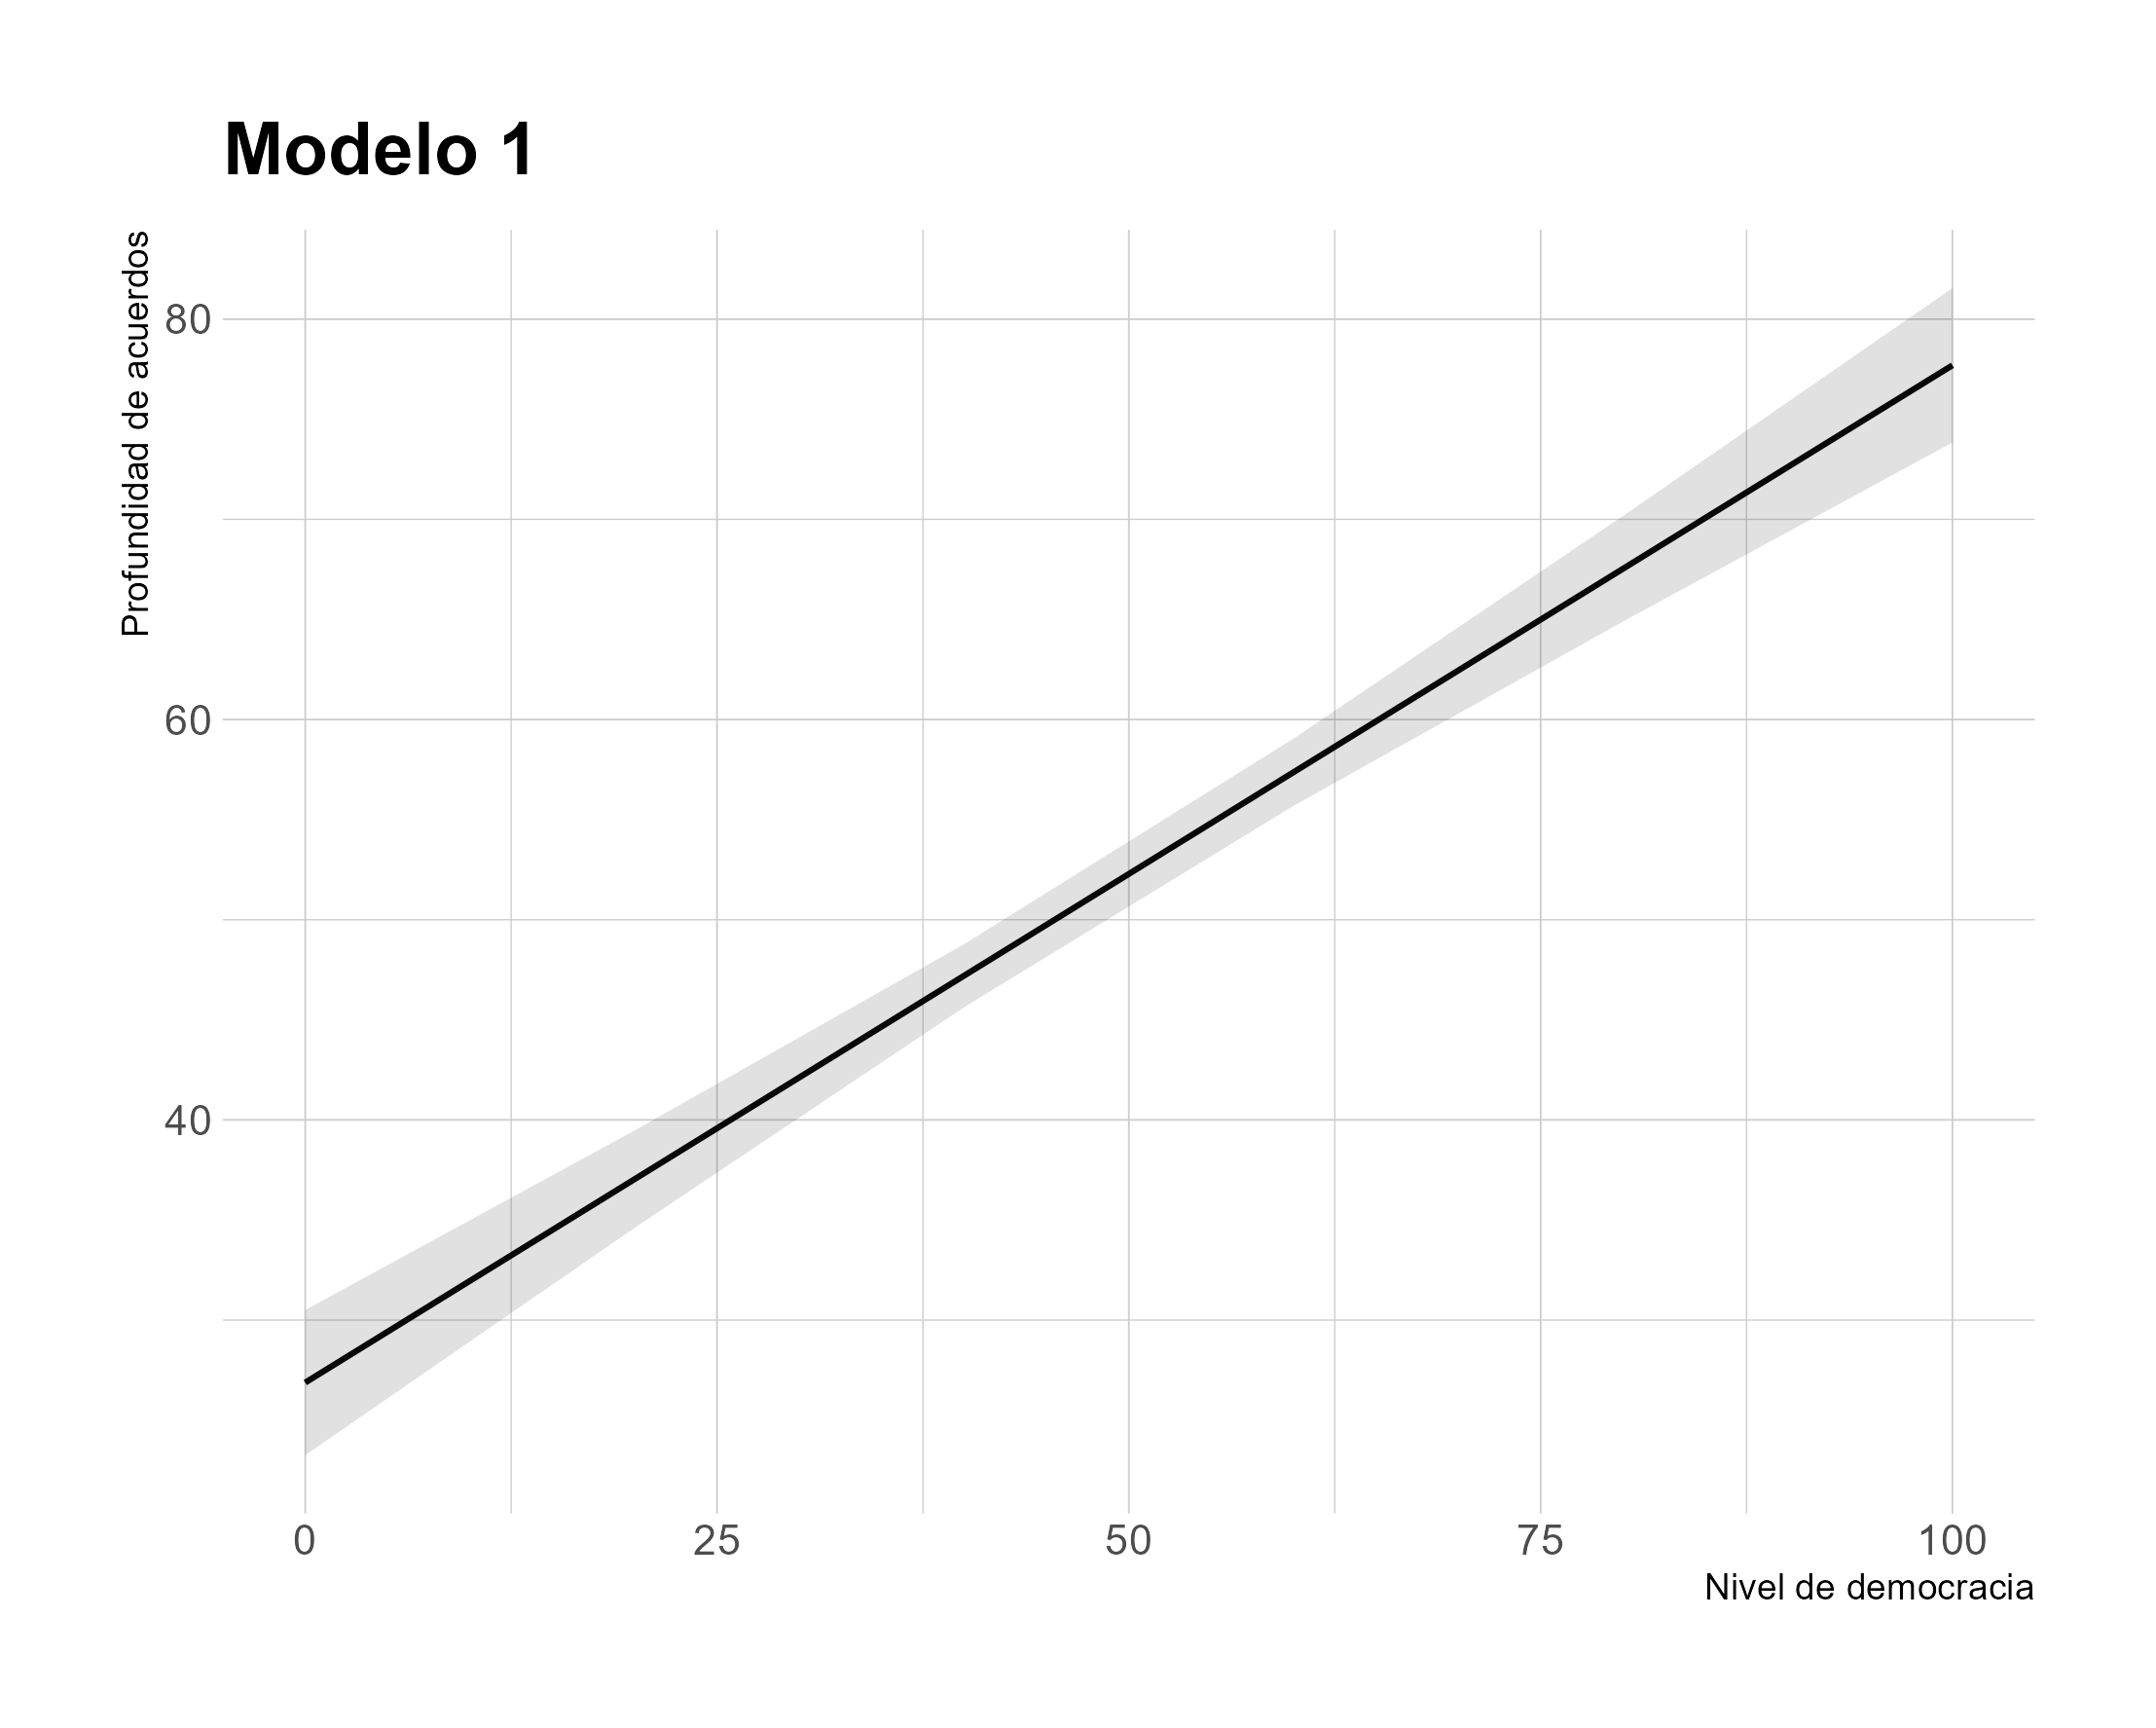
\includegraphics[width=.316\linewidth]{../01.Figures/figura_4a}}
  \subfloat{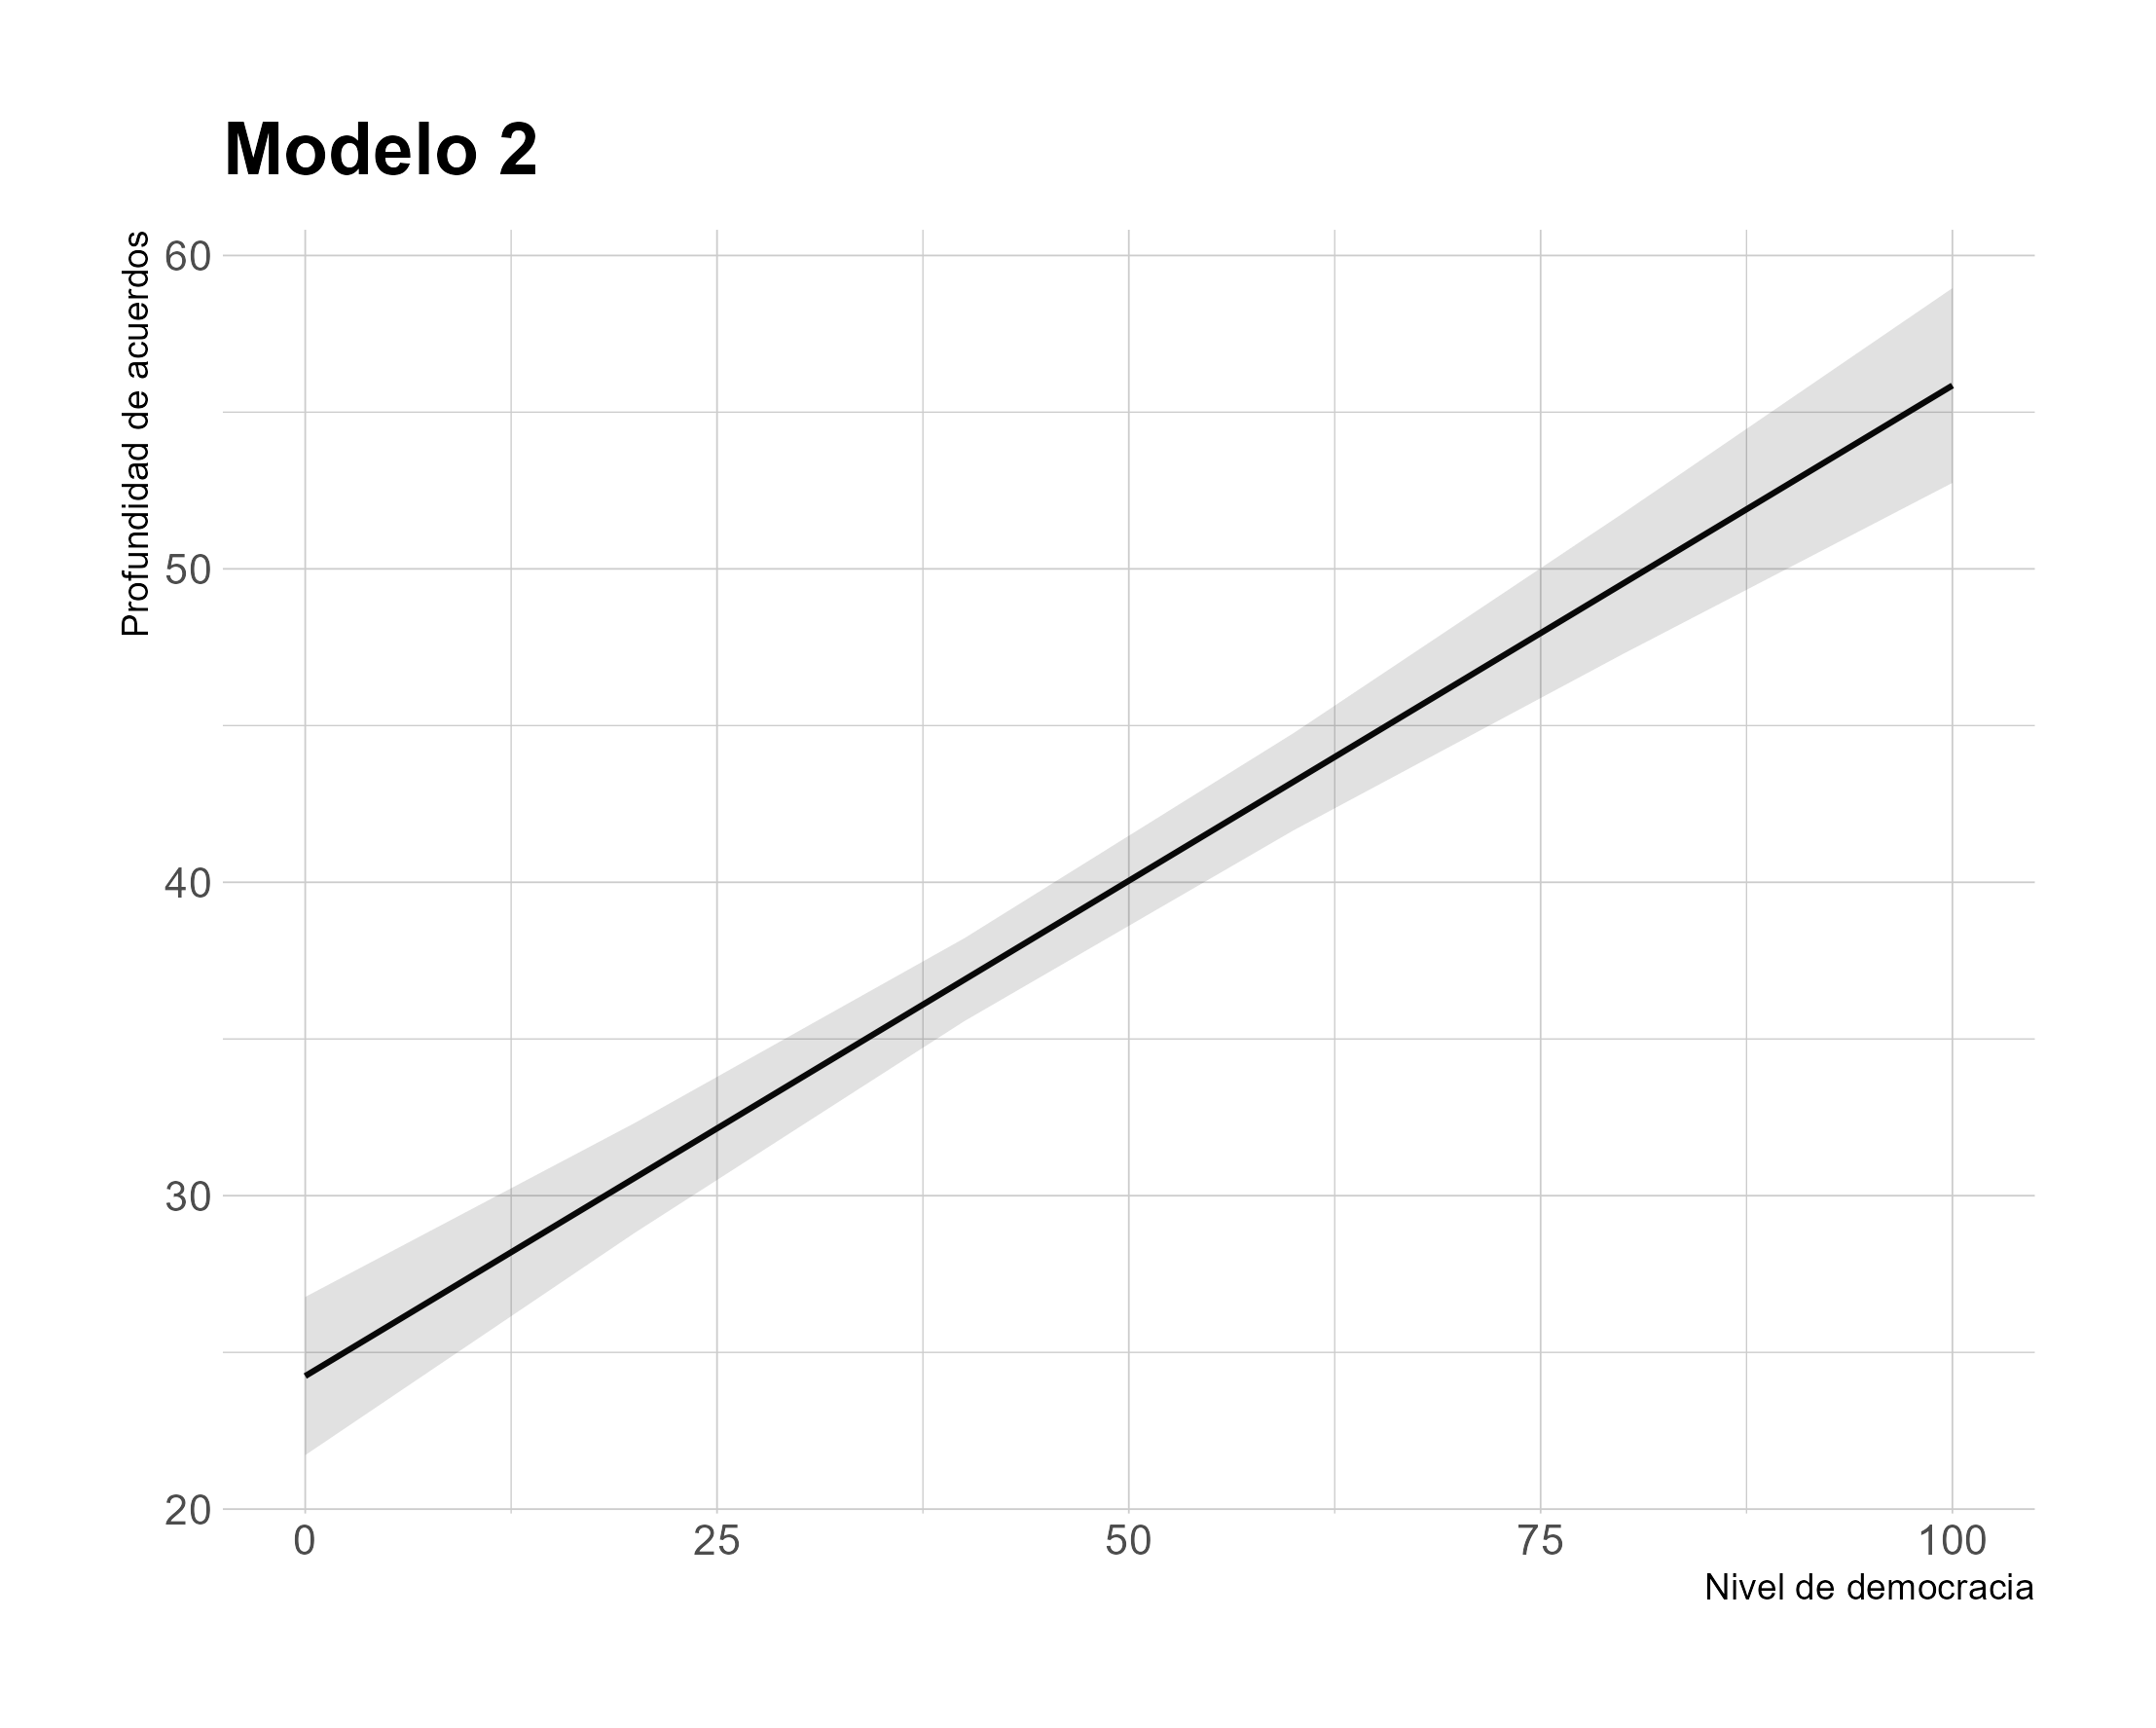
\includegraphics[width=.316\linewidth]{../01.Figures/figura_4b}}
  \subfloat{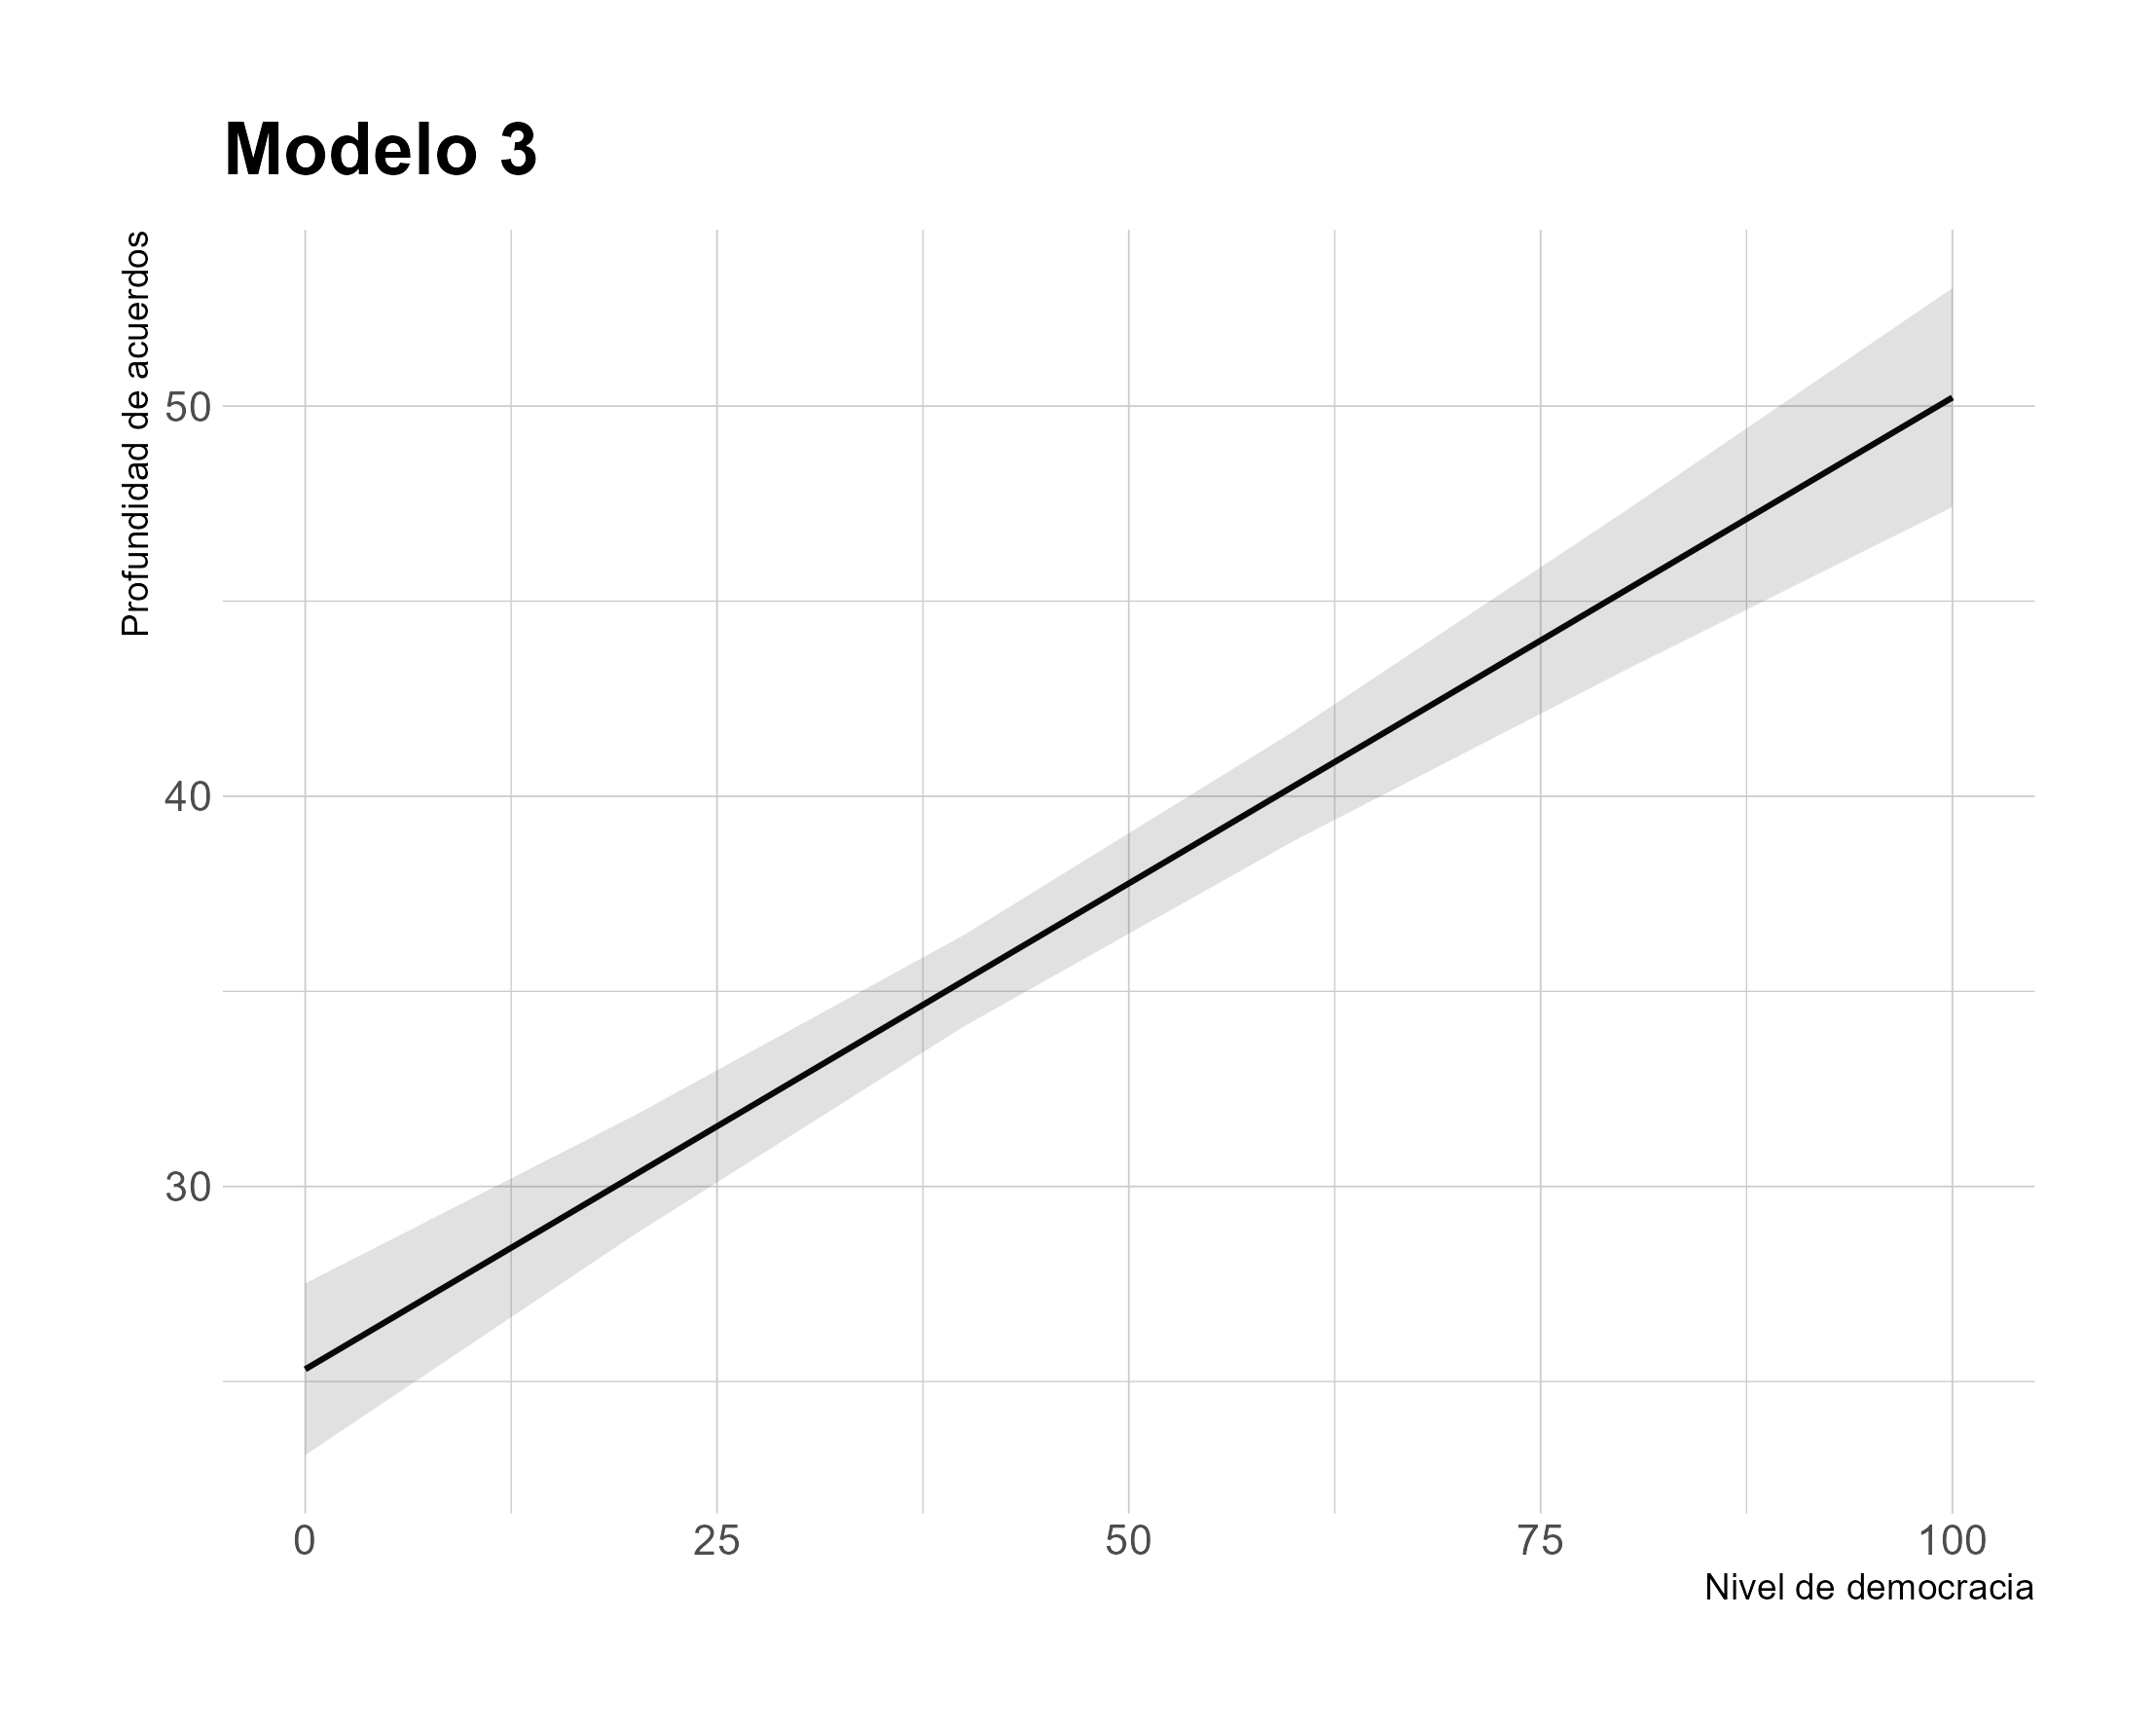
\includegraphics[width=.316\linewidth]{../01.Figures/figura_4c}}\\
   \subfloat{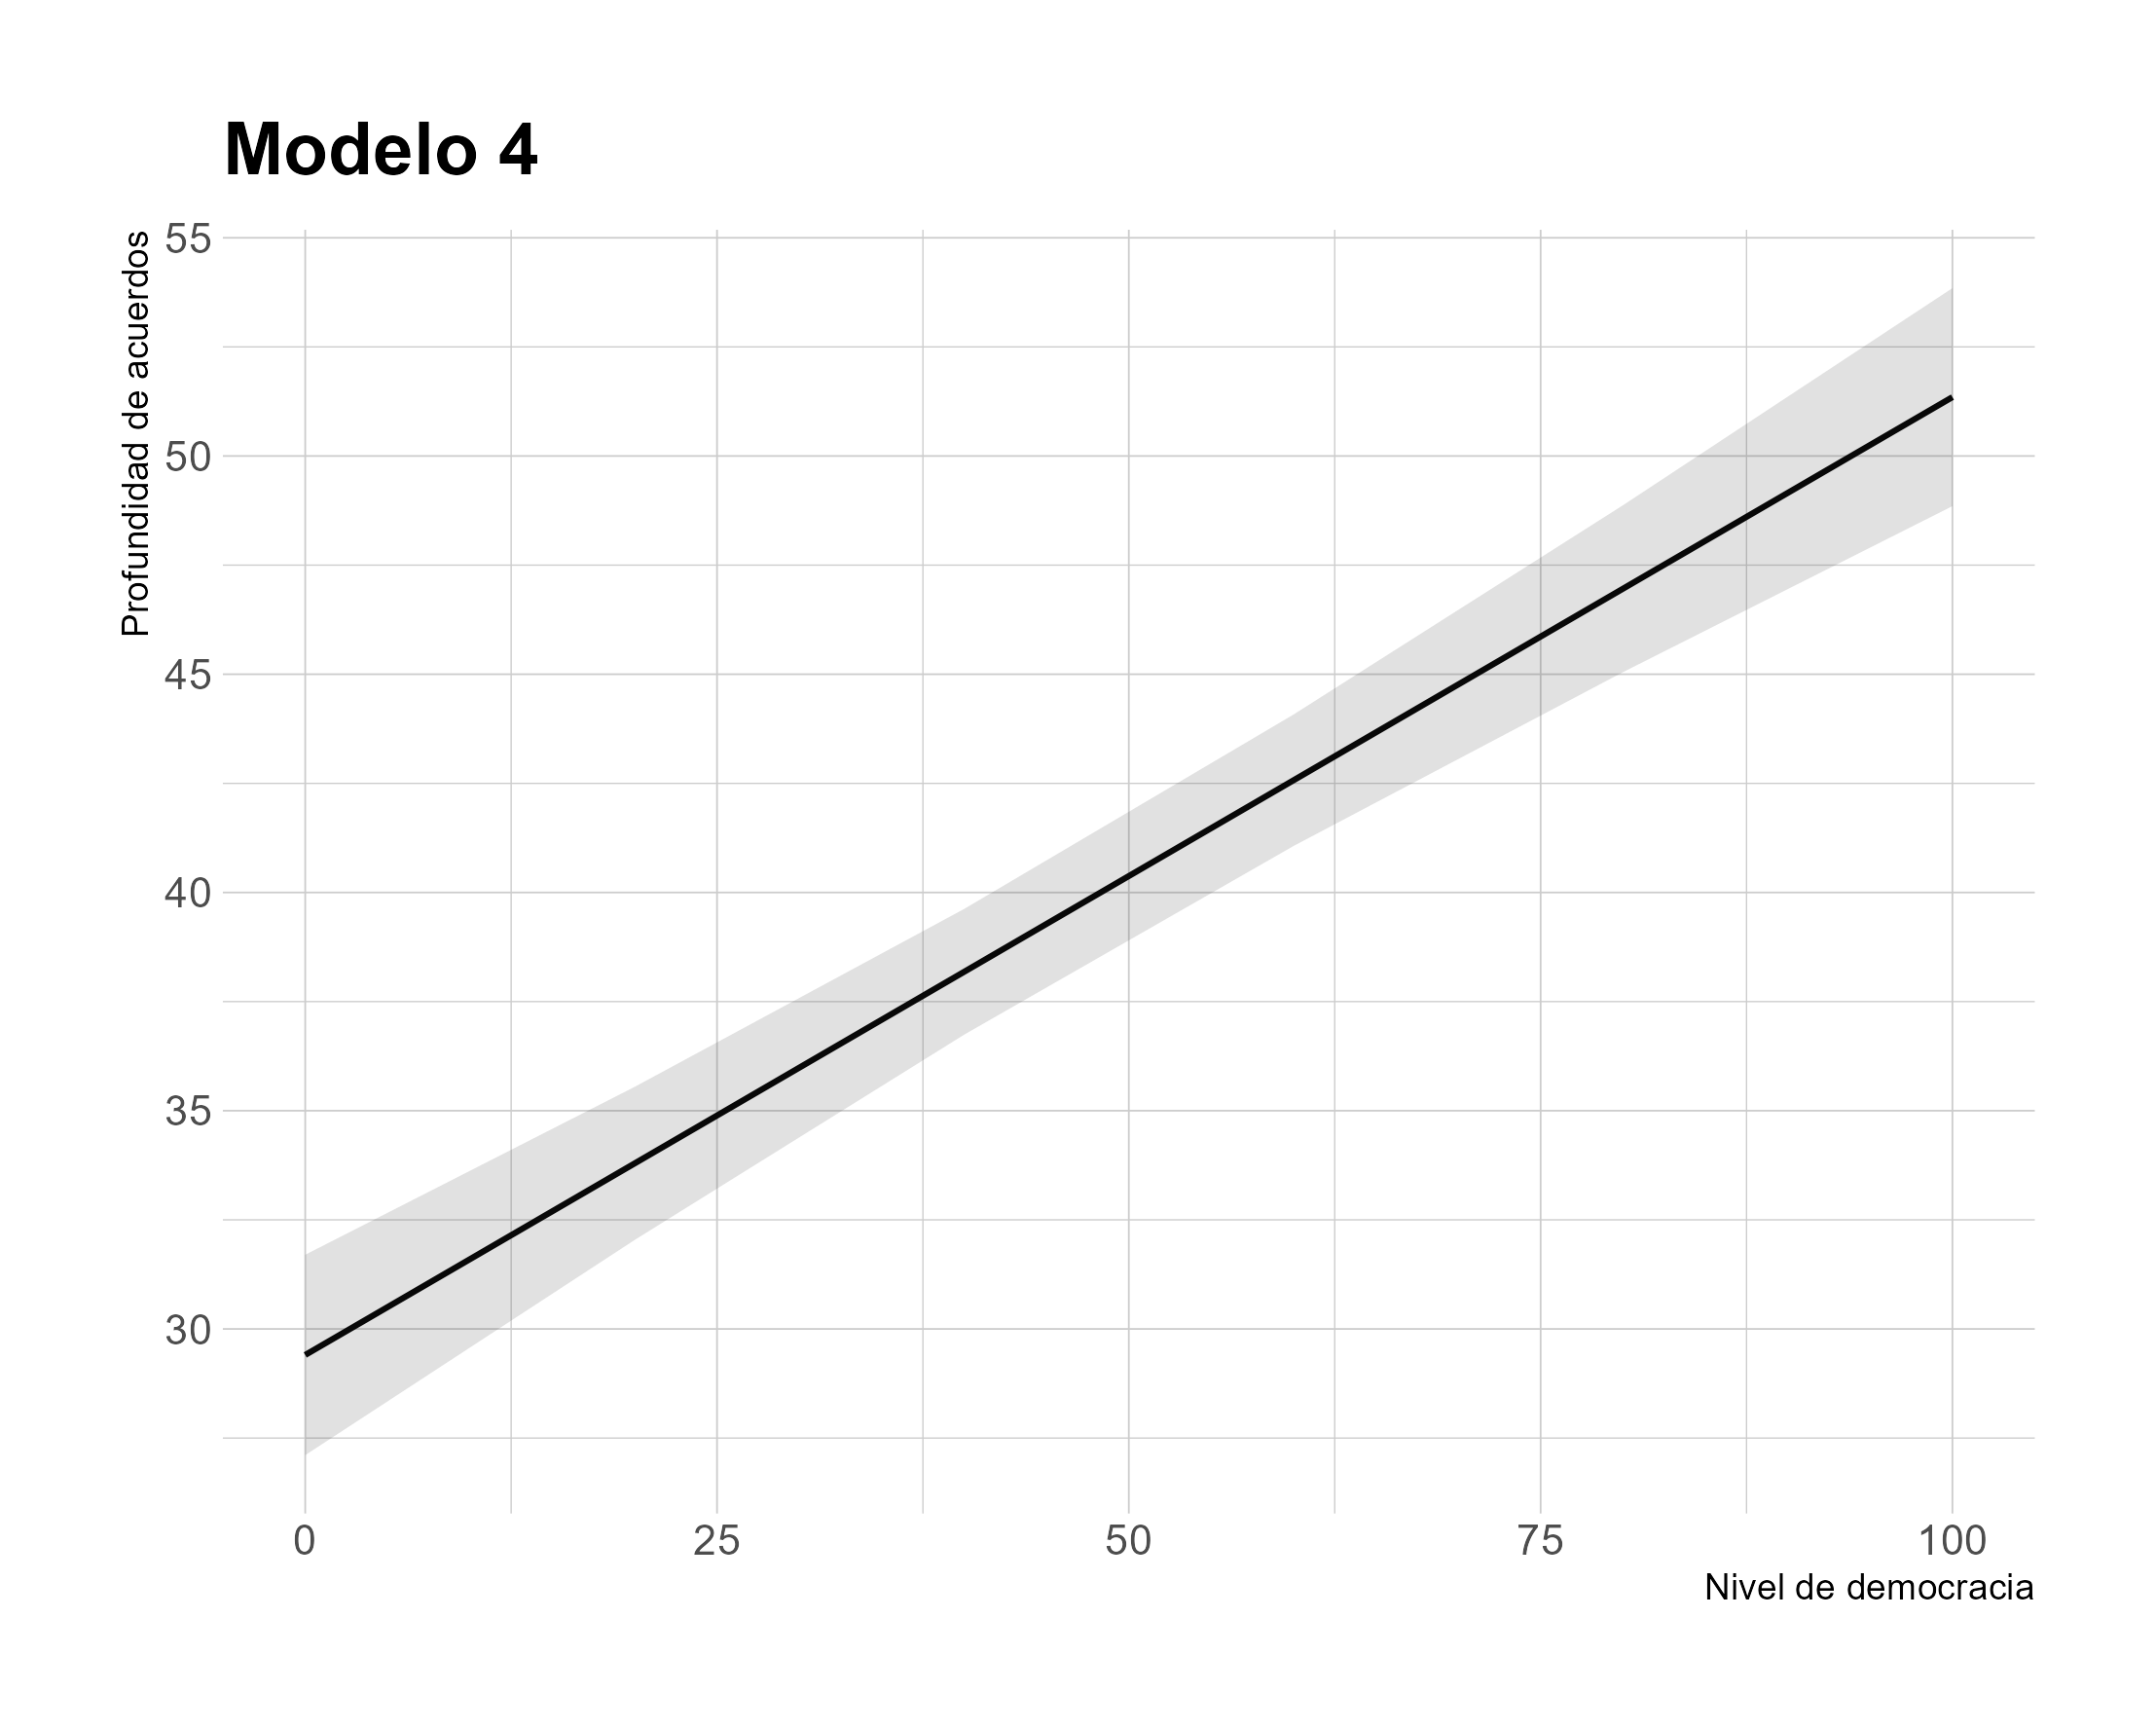
\includegraphics[width=.316\linewidth]{../01.Figures/figura_4d}}
   \subfloat{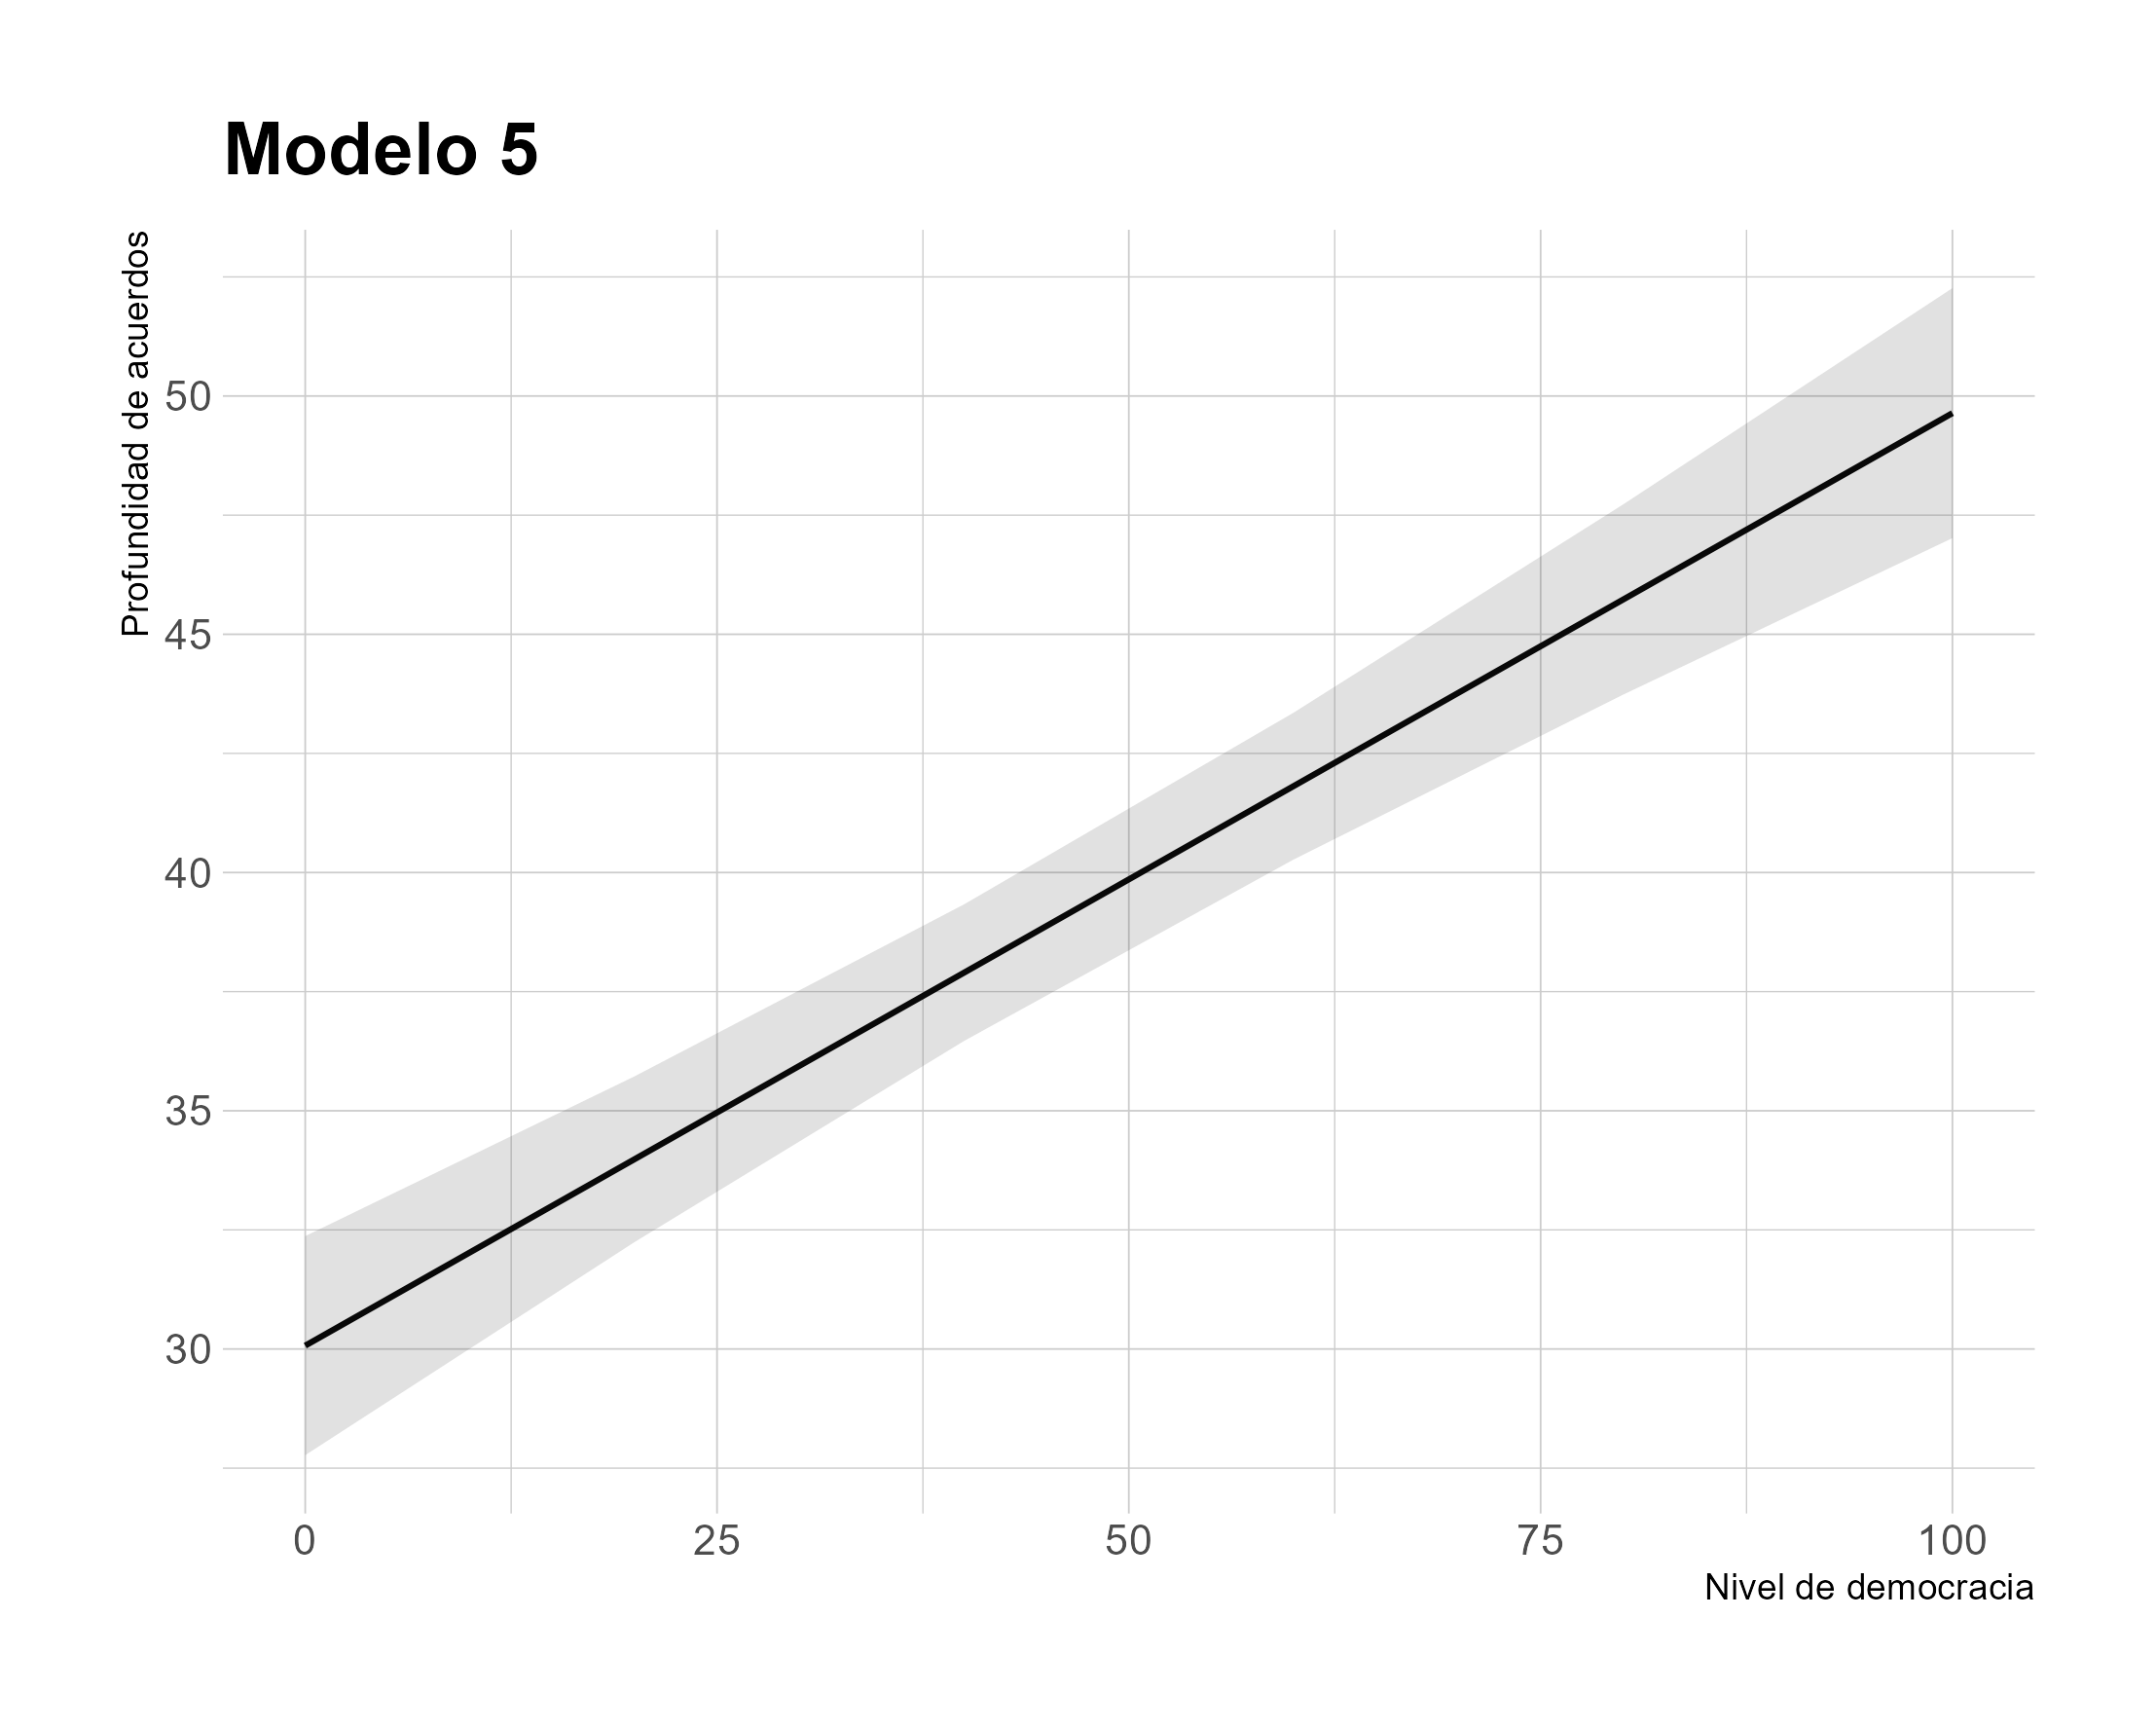
\includegraphics[width=.316\linewidth]{../01.Figures/figura_4e}}
  \\ \smallskip\noindent\scriptsize Fuente: Estimación propia con base en DESTA (2022) y Coppedge et al. (2022).
\end{figure*}

\justify{Al evaluar las especificaciones del modelo V en particular, no se advierten problemas severos de colinealidad, con la excepción de la variable respecto al período, la cual es problemática en algunas de sus categorías (períodos a partir de 1990 presentan valores superiores a cinco). Considerando la importancia que presenta el período en término analíticos, por sobre sus problemas de colinealidad, en vez de ser excluida del análisis su efecto es evaluado como un posible efecto interviniente sobre la democracia, con lo que se opta por asumir la colinealidad antes que eliminar la variable periodo. La estimación presenta problemas de heterocedasticidad, pero no problemas de linealidad de la variable democracia, con lo que se descarta la presencia de más de una tendencia en el efecto democrático sobre la profundidad democrático\footnote{El valor $p$ del término lineal de democracia es inferior a 0,000, mientras que al incluir un término cuadrático es $p = 0,177$.}. Los valores influyentes varían entre seis y siete casos, de un total de 692, por lo tanto, no tiene sentido eliminar observaciones\footnote{Mayores detalles disponibles en anexo.}.}

\justify{Considerando los diagnósticos obtenidos, no resulta necesario realizar demasiados ajustes a las estimaciones obtenidas (Gelman y Hill, 2017), salvo en el respecto a cómo abordar el efecto de los períodos, que tiende a aumentar con el paso del tiempo, y al papel que tienen los acuerdos con la UE, que si bien marca una diferencia es menor a lo que se esperaría. Para analizar estas consideraciones, se estudia un posible efecto de interviniente de los períodos y la presencia de acuerdos con la UE en la relevancia de la democracia sobre la profundidad de acuerdos. Si bien esto implica colinealidad, la manera en cómo se presentan los datos y su vinculación con la teoría respaldan esta decisión (Jaccard y Turrisi, 2003). Sin embargo, la inclusión de estos ajustes no produce los resultados esperados y se descarta la presencia de un posible efecto interviniente en ambos casos\footnote{Información disponible en anexo.}.}

\justify{Adicionalmente, evaluamos un potencial efecto multinivel mediante la inclusión de interceptos diferenciados por medio de una estructura anidada en que se diferencia la inclusión de un acuerdo con la UE dependiendo de distintos períodos. En el primer escenario, la presencia de este tipo de tratado incide en una mayor profundización hasta la década de 1990, mientras que a partir de los 2000, su bien los acuerdos con el bloque europeo tienden a incidir en mayores compromisos alcanzados, tratados que no consideran a este organismo supranacional como contraparte aumentan su mayor incidencia. Es decir, el efecto período tiene una incidencia bastante importante en ir diluyendo las diferencias entre si la UE era una contraparte o no (Figura 5 y Anexo 2).}

\begin{figure}[h!]
\captionsetup[subfigure]{labelformat=empty}
  \centering
  \smallskip\noindent\small Figura 5 \\ Profundidad de acuerdos, según período y acuerdo UE --- Modelo anidado
   \subfloat{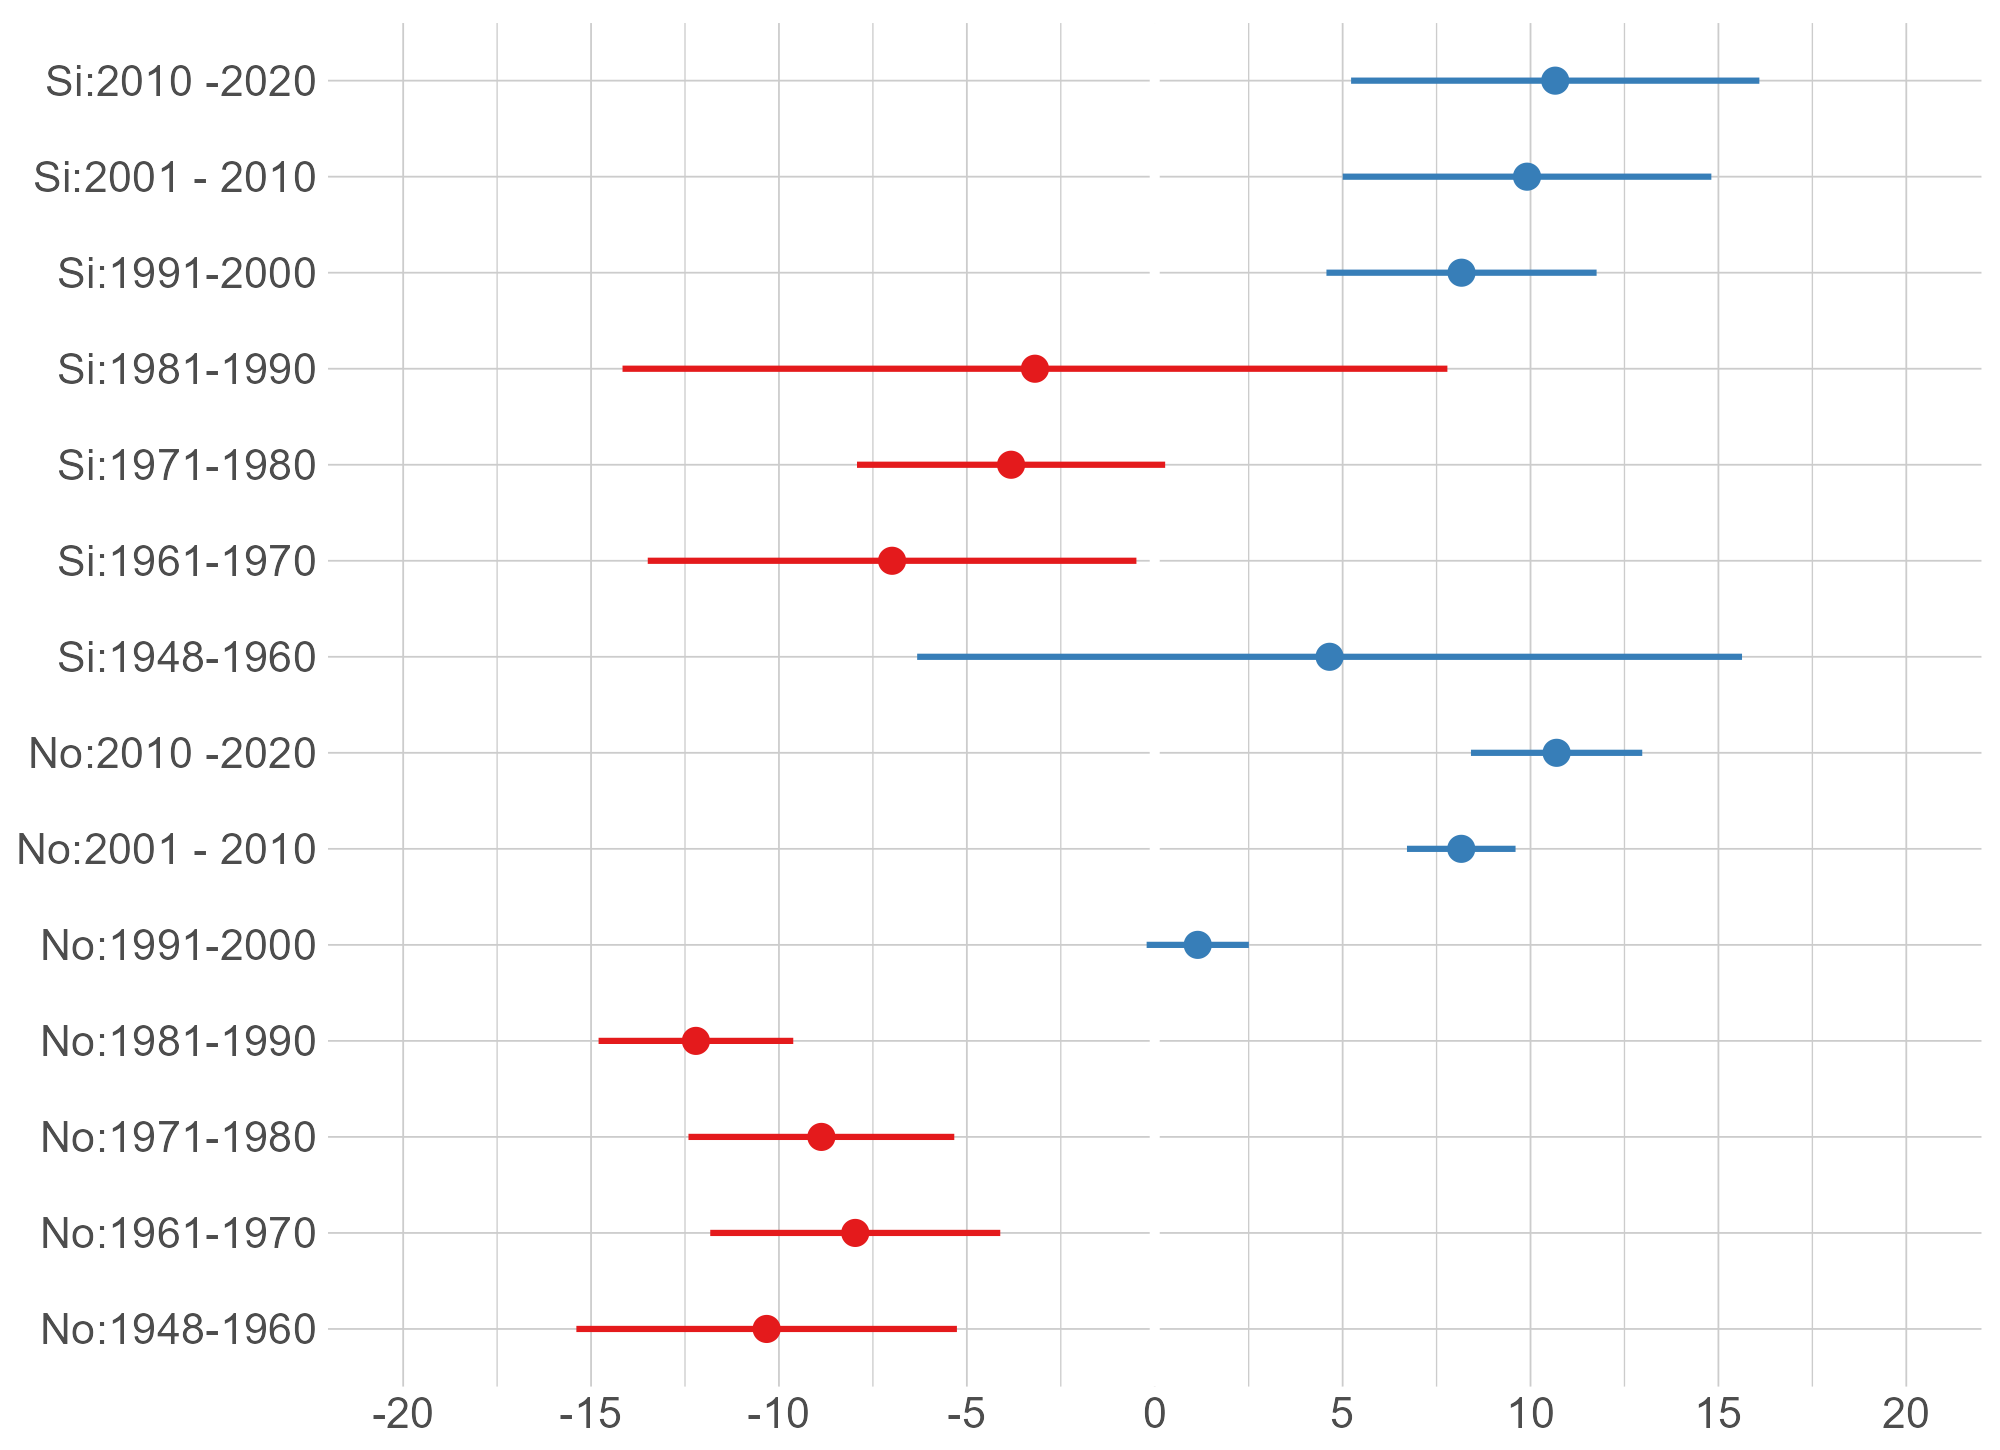
\includegraphics[width=.99\linewidth]{../01.Figures/figura_5}}
  \\ \smallskip\noindent\scriptsize Fuente: Estimación propia con base en DESTA (2022) y Coppedge et al. (2022).
\end{figure}

\justify{Una segunda estimación considera tanto el período como constante y el efecto de la presencia de un acuerdo con la UE como pendiente en cada intercepto (Gelman y Hill, 2017). En este caso, el efecto período muestra la importancia de lo que ocurre de manera posterior a 1990 es relevante, pero que al mismo tiempo el impacto de acuerdos como los de la UE tienden a diluirse en el tiempo, o al menos a atenuarse. Esto podría indicar que el papel de tratados de ese tipo responde esencialmente a lo que es una lógica propia de la década de 1990, con la preeminencia de las ideas que enfatizan la importancia de la democracia y el libre mercado, que comienza a disminuir con la década de los 2000. No sería, por cierto, una presencia de cambios abruptos, sino más bien a transformaciones que presentan características más bien graduales (Figura 6 y Anexo 2).}

\begin{figure}[h!]
\captionsetup[subfigure]{labelformat=empty}
  \centering
  \smallskip\noindent\small Figura 6 \\ Profundidad de acuerdos, según período y acuerdo UE
   \subfloat{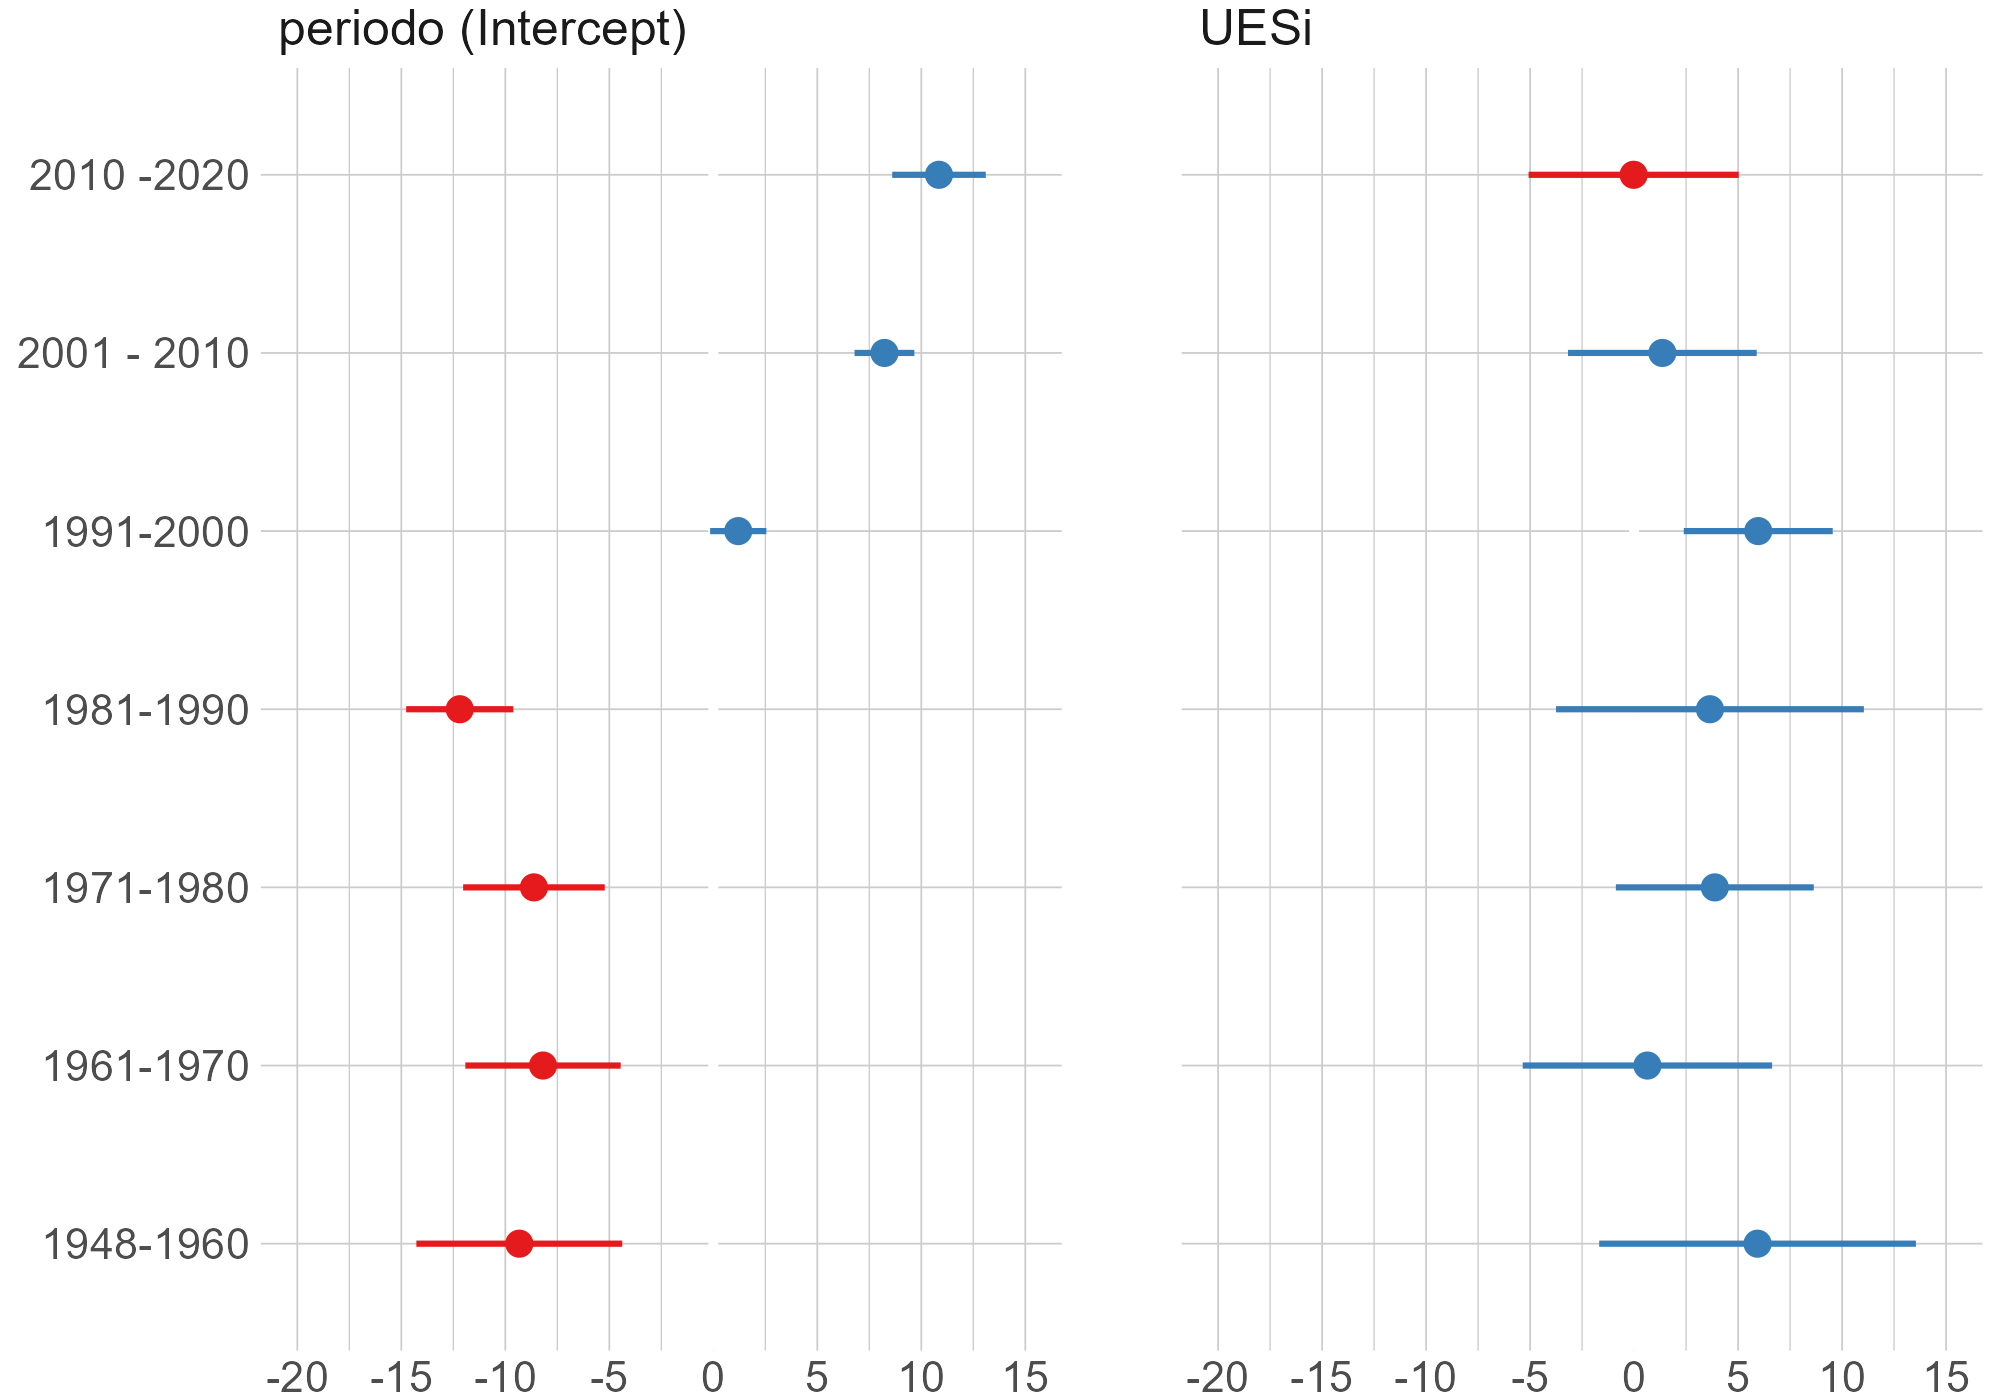
\includegraphics[width=.99\linewidth]{../01.Figures/figura_6}}
  \\ \smallskip\noindent\scriptsize Fuente: Estimación propia con base en DESTA (2022) y Coppedge et al. (2022).
\end{figure}

%%%%%%%%%%%%%%%%%%%%%%%%%%%%%%%%%%%%%%%%%%%%%%%%%%

\section[Conclusiones] {{\normalfont Conclusiones}}

%%%%%%%%%%%%%%%%%%%%%%%%%%%%%%%%%%%%%%%%%%%%%%%%%%

\justify{En relación con la hipótesis central planteada en el artículo, que es la relevancia que tiene el nivel democrático de las partes que concurrentes en la profundidad que alcancen los compromisos obtenidos en un acuerdo de libre comercio, esta es bastante importante, tomando en cuenta tanto el nivel de ajuste en la estimación como en la validez de su coeficiente. En ese sentido, los resultados tienden a coincidir con las referencias teóricas. Si bien mantienen un efecto lineal a lo largo de los distintos modelos estimados, lo que sería positivo desde el punto de vista de la ejecución técnica, los cambios que se van sucediendo al ir agregando variables, bastante importantes entre cada uno, hacen suponer el carácter interviniente otros regresores diferentes al nivel de democracia.}

\justify{Al incluir la presencia de un capítulo de inversiones, pero especialmente uno de propiedad intelectual, atenúan de manera importante el efecto que tiene el desarrollo democrático. Tomando en cuenta que el impacto de esta variable no cambia de manera sustantiva al incorporar variables como la presencia de un acuerdo con la UE o la diferenciación de acuerdo con las décadas en que se firmaron estos tratados, reafirman la importancia de considerar aquellos capítulos de acuerdos que buscan introducir un mayor nivel de desregulación, como lo reflejan el fortalecimiento de la propiedad intelectual y de la protección de inversiones. Es decir, refuerzan argumentos que van más en la línea que los acuerdos si bien tienden a acercarse a enfoques liberales de las relaciones internacionales, esto tiene más relación con los aspectos económicos que con la teoría de la paz democrática.}

\justify{Esta preminencia de la importancia que adquieren capítulos como la propiedad intelectual o la protección de las inversiones se releva aún más al toman en consideración la escasa relevancia que tiene variables de control que aparecieron importantes en la formulación de la pregunta de investigación, como lo fue la presencia de la UE como contraparte o la diferenciación entre períodos, cuando estas fueron evaluadas como posibles variables intervinientes.}

\justify{No obstante, al evaluar estos dos controles y su posible efecto de grupo, los resultados muestran la relevancia que tuvo la UE hasta 1990, en que los acuerdos en que esta participaba efectivamente tenían una diferencia significativa si se comparaban con aquellos tratados en los que esta estaba ausente. Lo que se muestra posteriormente no es que los acuerdos en que participaba el bloque europeo dejaran de tener profundidad, sino que otro tipo de acuerdos avanzaron más aceleradamente en ello.}

\justify{En ese sentido, si bien en el artículo se muestra la importancia que tiene la democracia en la profundidad que adquiere un acuerdo de libre comercio, esta aparece secundaria, en relación con aquellos aspectos que se relacionan con la liberalización de los mercados. En este sentido, un matiz que se introduce a partir de los resultados obtenidos, esta importancia si bien existe y es posible constatar, es un argumento que tiende a perder importancia a medida que transcurre el siglo XXI. Finalmente, cabe mencionar la problemática de los datos disponibles, que son de carácter observacional y que introducen sesgo en las estimaciones obtenidas\footnote{Para más detalles véase González-Bustamante (2022).}. Si bien ello tiene que ver con que los datos disponibles van cambiando a medida que DESTA va actualizando la información sobre tratados de libre comercio (Baccini et al., 2014), en investigaciones futuras se recomienda considerar la factibilidad de aplicar técnicas que reduzcan o atenúen en sesgo introducido por el uso de datos observacionales.}

%%%%%%%%%%%%%%%%%%%%%%%%%%%%%%%%%%%%%%%%%%%%%%%%%%

\section{{\normalfont Referencias}}

%%%%%%%%%%%%%%%%%%%%%%%%%%%%%%%%%%%%%%%%%%%%%%%%%%

\begin{list}{}%
{\leftmargin=1em \itemindent=-1em}

\item{\small Allee, T., {\itshape \&} Elsig, M. (2016). Why do some international institutions contain strong dispute settlement provisions? New evidence from preferential trade agreements. {\itshape The Review of International Organizations, 11}(1), 89-120.}

\item{\small Alle, T., {\itshape \&} Elsig, M. (2019). Are the Contents of International Treaties Copied and Pasted? Evidence from Preferential Trade Agreements. {\itshape International Studies Quarterly, 63}(3), 603-613.}

\item{\small Anderer, C., Dür, A., {\itshape \&} Lechner, L. (2020). Trade policy in a “GVC World”: Multinational corporations and trade liberalization. {\itshape Business and Politics, 22}(4), 639-666.}

\item{\small Baccini, L., Dür, A., {\itshape \&} Elsig, M. (2014). The Design of International Trade Agreements: Introducing a New Database. {\itshape The Review of International Organizations, 9}(3), 353-375.}

\item{\small Baldwin, D. (1980). Interdependence and power: a conceptual analysis. {\itshape International Organization, 34}(4), 471-506.}

\item{\small Bartolucci, F., Bacci, S., {\itshape \&} Gnaldi, M. (2016). Statistical Analysis of Questionnaires. Nueva York: CRC PRESS / Taylor {\itshape \&} Francis Group.}

\item{\small Bliss, H., {\itshape \&} Russett, B. (1998). Democratic Trading Partners: The Liberal Connection, 1962-1989. {\itshape The Journal of Politics, 60}(4), 1126-1147.}

\item{\small Bull, B. (2008). Policy Networks and Business Participation in Free Trade Negotiations in Chile. {\itshape Journal of Latin American Studies, 40}(2), 195-224.}

\item{\small Burri, M., {\itshape \&} Polanco, R. (2020). Digital Trade Provisions in Preferential Trade Agreements: Introducing a New Dataset. {\itshape Journal of International Economic Law, 23}(1), 187-220.}

\item{\small Càrrere, C., Olarreaga, M., {\itshape \&} Raess, D. (2022). Labor clauses in trade agreements: Hidden protectionism? The {\itshape Review of International Organization, 17}, 453-483.}

\item{\small Chaisse, J. (2012). TPP Agrrement: towards innovations in investment rule-making. En C. Lim, D. K. Elms, {\itshape \&} P. Low (Eds.), {\itshape The Transpacific-Partnership. A quest for a Twenty-first-Century Trade Agreement}. Cambridge: Cambirdge Universtiy Press.}

\item{\small Chang , E., {\itshape \&} Wen-Chin, W. (2016). Preferential Trade Agreements, Income Inequality, and Authoritarian Survival. {\itshape Political Research Quarterly, 69}(2), 281-294.}

\item{\small Cuevas R. (2022). Democracia y profundidad de los compromisos adquiridos en acuerdos de libre comercio (1948-2020). {\itshape Estudios Internacionales, 54}(203), 35-60.}

\item{\small Cuevas, R. (2019). Reformas de Mercado y Acuerdos Comerciales en América Latina (1970-2015). {\itshape Revista mexicana de ciencias políticas y sociales, 64}(237), 377-407.}

\item{\small Cuevas, R., {\itshape \&} Morillo-Remesnitzky, J. (2020). ¿Todos los caminos llevan a Washington? Trayectorias de América Latina hacia un Acuerdo de Libre Comercio con los Estados Unidos (1990-2015). {\itshape Revista Chilena de Derecho y Ciencia Política, 11}(2), 206-236.}

\item{\small Coppedge, M., Gerring, J., Knutsen, C. H., Lindberg, S. I., Teorell, J., Alizada, N., Altman, D., Bernhard, M., Cornell, A., Fish, M. S., Gastaldi, L., Gjerløw, H., Glynn, A., Grahn, S., Hicken, A., Hindle, G., NinaIlchenko, Kinzelbach, K., Krusell, J., … Ziblatt, D. (2022). V-Dem Country-Year Dataset v12 [Dataset]. Varieties of Democracy Institute, University of Gothenburg.}

\item{\small DESTA (2022). Design of Trade Agreements (DESTA) Database. Disponible en: \href{https://www.designoftradeagreements.org/downloads}{\textcolor{blue}{https://www.designoftradeagreements.org}} (consultado el 15 de julio de 2022).}

\item{\small Díez-Medrano, J. (2018). Beliefs and trade union support for trade liberalisation in the US and the UK: the AFL-CIO and the TUC compared. {\itshape Journal of International Relations and Development, 21}, 769-797.}

\item{\small Dür, A., {\itshape \&} De Briève, D. (2007). Inclusion without Influence? NGOs in European Trade Policy. {\itshape Journal of Public Policy, 27}(1), 79-101.}

\item{\small Elsig , M., {\itshape \&} Klotz, S. (2021). Digital Trade Rules in Preferential Trade. Agreements: Is There a WTO Impact? {\itshape Global Policy, 12}(S4), 25-36.}

\item{\small Frankel, S. (2012). The intellectual property chapter in the TPP. En C. Lim, D. K. Elms, {\itshape \&} P. Low (Eds.), {\itshape The Trans-Pacific Partnership. A Quest for a Twenty-first-Century Trade Agreement}. Cambdrige: Camdridge University Press.}

\item{\small Gartzke, E. (2007). The Capitalist Peace. {\itshape American Journal of Political Science, 5}(1), 166-191.}

\item{\small Gelman, A., {\itshape \&} Hill, J. (2017). {\itshape Data Analysis Using Regression and Multilevel / Hierarchical Models (17th printing)}. Nueva York: Cambridge University Press.}

\item{\small Giles, R. H. (1970). The Role of Trade in International Relations. {\itshape International Relations, 3}(8), 565-577.}

\item{\small Giuliano, P., Mishra, P., {\itshape \&} Spilimbergo, A. (2010). Democracy and Reforms: Evidence from a New Dataset. WP/10/73. IMF Working Paper.}

\item{\small González-Bustamente, Bastián (2022), Métodos cuantitativos para estudiar a las élites: Aplicaciones prácticas, sesgos y potencialidades. {\itshape Revista Chilena de Derecho y Ciencia Política, 13}(2), 12-44. }

\item{\small Harrel, F. (2001). {\itshape Regression Modeling Strategies: with Applications to Linear Models, Logistic Regression, and Survival Analysis}. Nueva York: Springer.}

\item{\small Hulse, M. (2017). Actorness and trade negotiating outcomes: West Africa and the SADC Group in negotiations for Economic Partnership Agreements. {\itshape International Relations, 32}(1), 39-59.}

\item{\small Jaccard, J., {\itshape \&} Turrisi, R. (2003). {\itshape Interaction Effects in Multiple Regression}. Texas: SAGE.}

\item{\small Jo, H., {\itshape \&} Namgung, H. (2012). Dispute Settlement Mechanisms in Preferential Trade Agreements: Democracy, Boilerplates, and the Multilateral Trade Regime. {\itshape Journal of Conflict Resolution, 56}(6), 1014-1068.}

\item{\small Lechner, L. (2016). The domestic battle over the design of non-trade issues in preferential trade agreements. {\itshape Review of International Political Economy, 23}(5), 840-871.}

\item{\small Lenz, T. (2012). Spurred Emulation: The EU and Regional Integration in Mercosur and SADC. {\itshape West European Politics, 35}(1), 155-173.}

\item{\small Lenz, T. (2021). {\itshape Interorganizational Diffusion in International Relations: Regional Institutions and the Role of the European Union}. Oxford: Oxford University Press.}

\item{\small Liu, X., {\itshape \&} Ornelas, E. (2014). Free Trade Agreements and the Consolidation of Democracy. {\itshape American Economic Journal: Macroeconomics, 6}(2), 29-70.}

\item{\small Mansfield, E., {\itshape \&} Milner, H. (2012). {\itshape Votes, Vetoes, and the Political Economy of International Trade Agreements}. Princeton: Princeton University Press.}

\item{\small Mansfield, E., Milner, H., {\itshape \&} Rosendorff, P. (2002). Why Democracies Cooperate More: Electoral Control and International Trade Agreements. {\itshape International Organization, 56}(3), 477-513.}

\item{\small McMillan, S. (1997). Interdependence and conflict. {\itshape Mershon International Studies Review 41}(1), 33-58.}

\item{\small Morin, J.-F., Dür, A., {\itshape \&} Lechner, L. (2018). Mapping the Trade and Environment Nexus: Insights from a New Data Set. {\itshape Global Environmental Politics, 18}(1), 122-139.}

\item{\small Morin, J., {\itshape \&} Surbeck, J. (2020). Mapping the New Frontier of International IP Law: Introducing a TRIPs-plus Dataset. {\itshape World Trade Review, 19}(1), 109-122.}

\item{\small Polacheck , S. (1997). Why Democracies Cooperate More and Fight Less: The Relationship Between International Trade and Cooperation. {\itshape Review of International Economics, 5}(3), 295-309.}

\item{\small Putnam, R. (1988). Diplomacy and Domestic Politics: The Logic of Two-Level Games. {\itshape International Organization, 42}(3), 427-460.}

\item{\small Raess, D., {\itshape \&} Sari, D. (2018). Labor Provisions in Trade Agreements (LABPTA): Introducing a New Dataset. {\itshape Global Policy, 9}(4), 451-466.}

\item{\small Ravenhill, J. (2011). {\itshape Global Political Economy}. Nueva York: Oxford University Press.}

\item{\small Raykov, T., {\itshape \&} Marcoulides, G. A. (2018). {\itshape A Course in Item Response Theory and Modeling with Stata}. Texas: Stata Press.}

\item{\small Ruggie, J. (1982). International Regimes, Transactions, and Change: Embedded Liberalism in the Postwar Economic Order. {\itshape International Organization, 36}(2), 379-415.}

\item{\small RTA-IS (2022). Regional Trade Agreements Database. Disponible en: \\ \href{https://rtais.wto.org/UI/PublicMaintainRTAHome.aspx}{\textcolor{blue}{https://rtais.wto.org}} (consultado el 11de julio de 2022).}

\item{\small Smith, N. R. (2015). The EU under a realist scope: Employing a neoclassical realist framework for the analysis of the EU’s Deep and Comprehensive Free Trade Agreement offer to Ukraine. {\itshape International Relations, 30}(1), 29-48.}

\item{\small WTO (2011). {\itshape World Trade Report: The WTO and preferential trade agreements: From co-existence to coherence}. Ginebra: World Trade Organization.}

\item{\small Velluti, S. (2020). {\itshape The Role of the EU in the Promotion of Human Rights and International Labour Standards in Its External Trade Relations}. Cham: Springer.}

\item{\small von Bülow, M. (2009). Networks of Trade Protest in the Americas: Toward a New Labor Internationalism? {\itshape Latin American Politics and Society, 51}(2), 1-28.}

\end{list}

%%%%%%%%%%%%%%%%%%%%%%%%%%%%%%%%%%%%%%%%%%%%%%%%%%

\section{{\normalfont Anexos}}

%%%%%%%%%%%%%%%%%%%%%%%%%%%%%%%%%%%%%%%%%%%%%%%%%%

\begin{figure*}[h!]
\captionsetup[subfigure]{labelformat=empty}
  \centering
  \smallskip\noindent\small Anexo 1 \\ Gráficos de diagnóstico del modelo V
   \subfloat{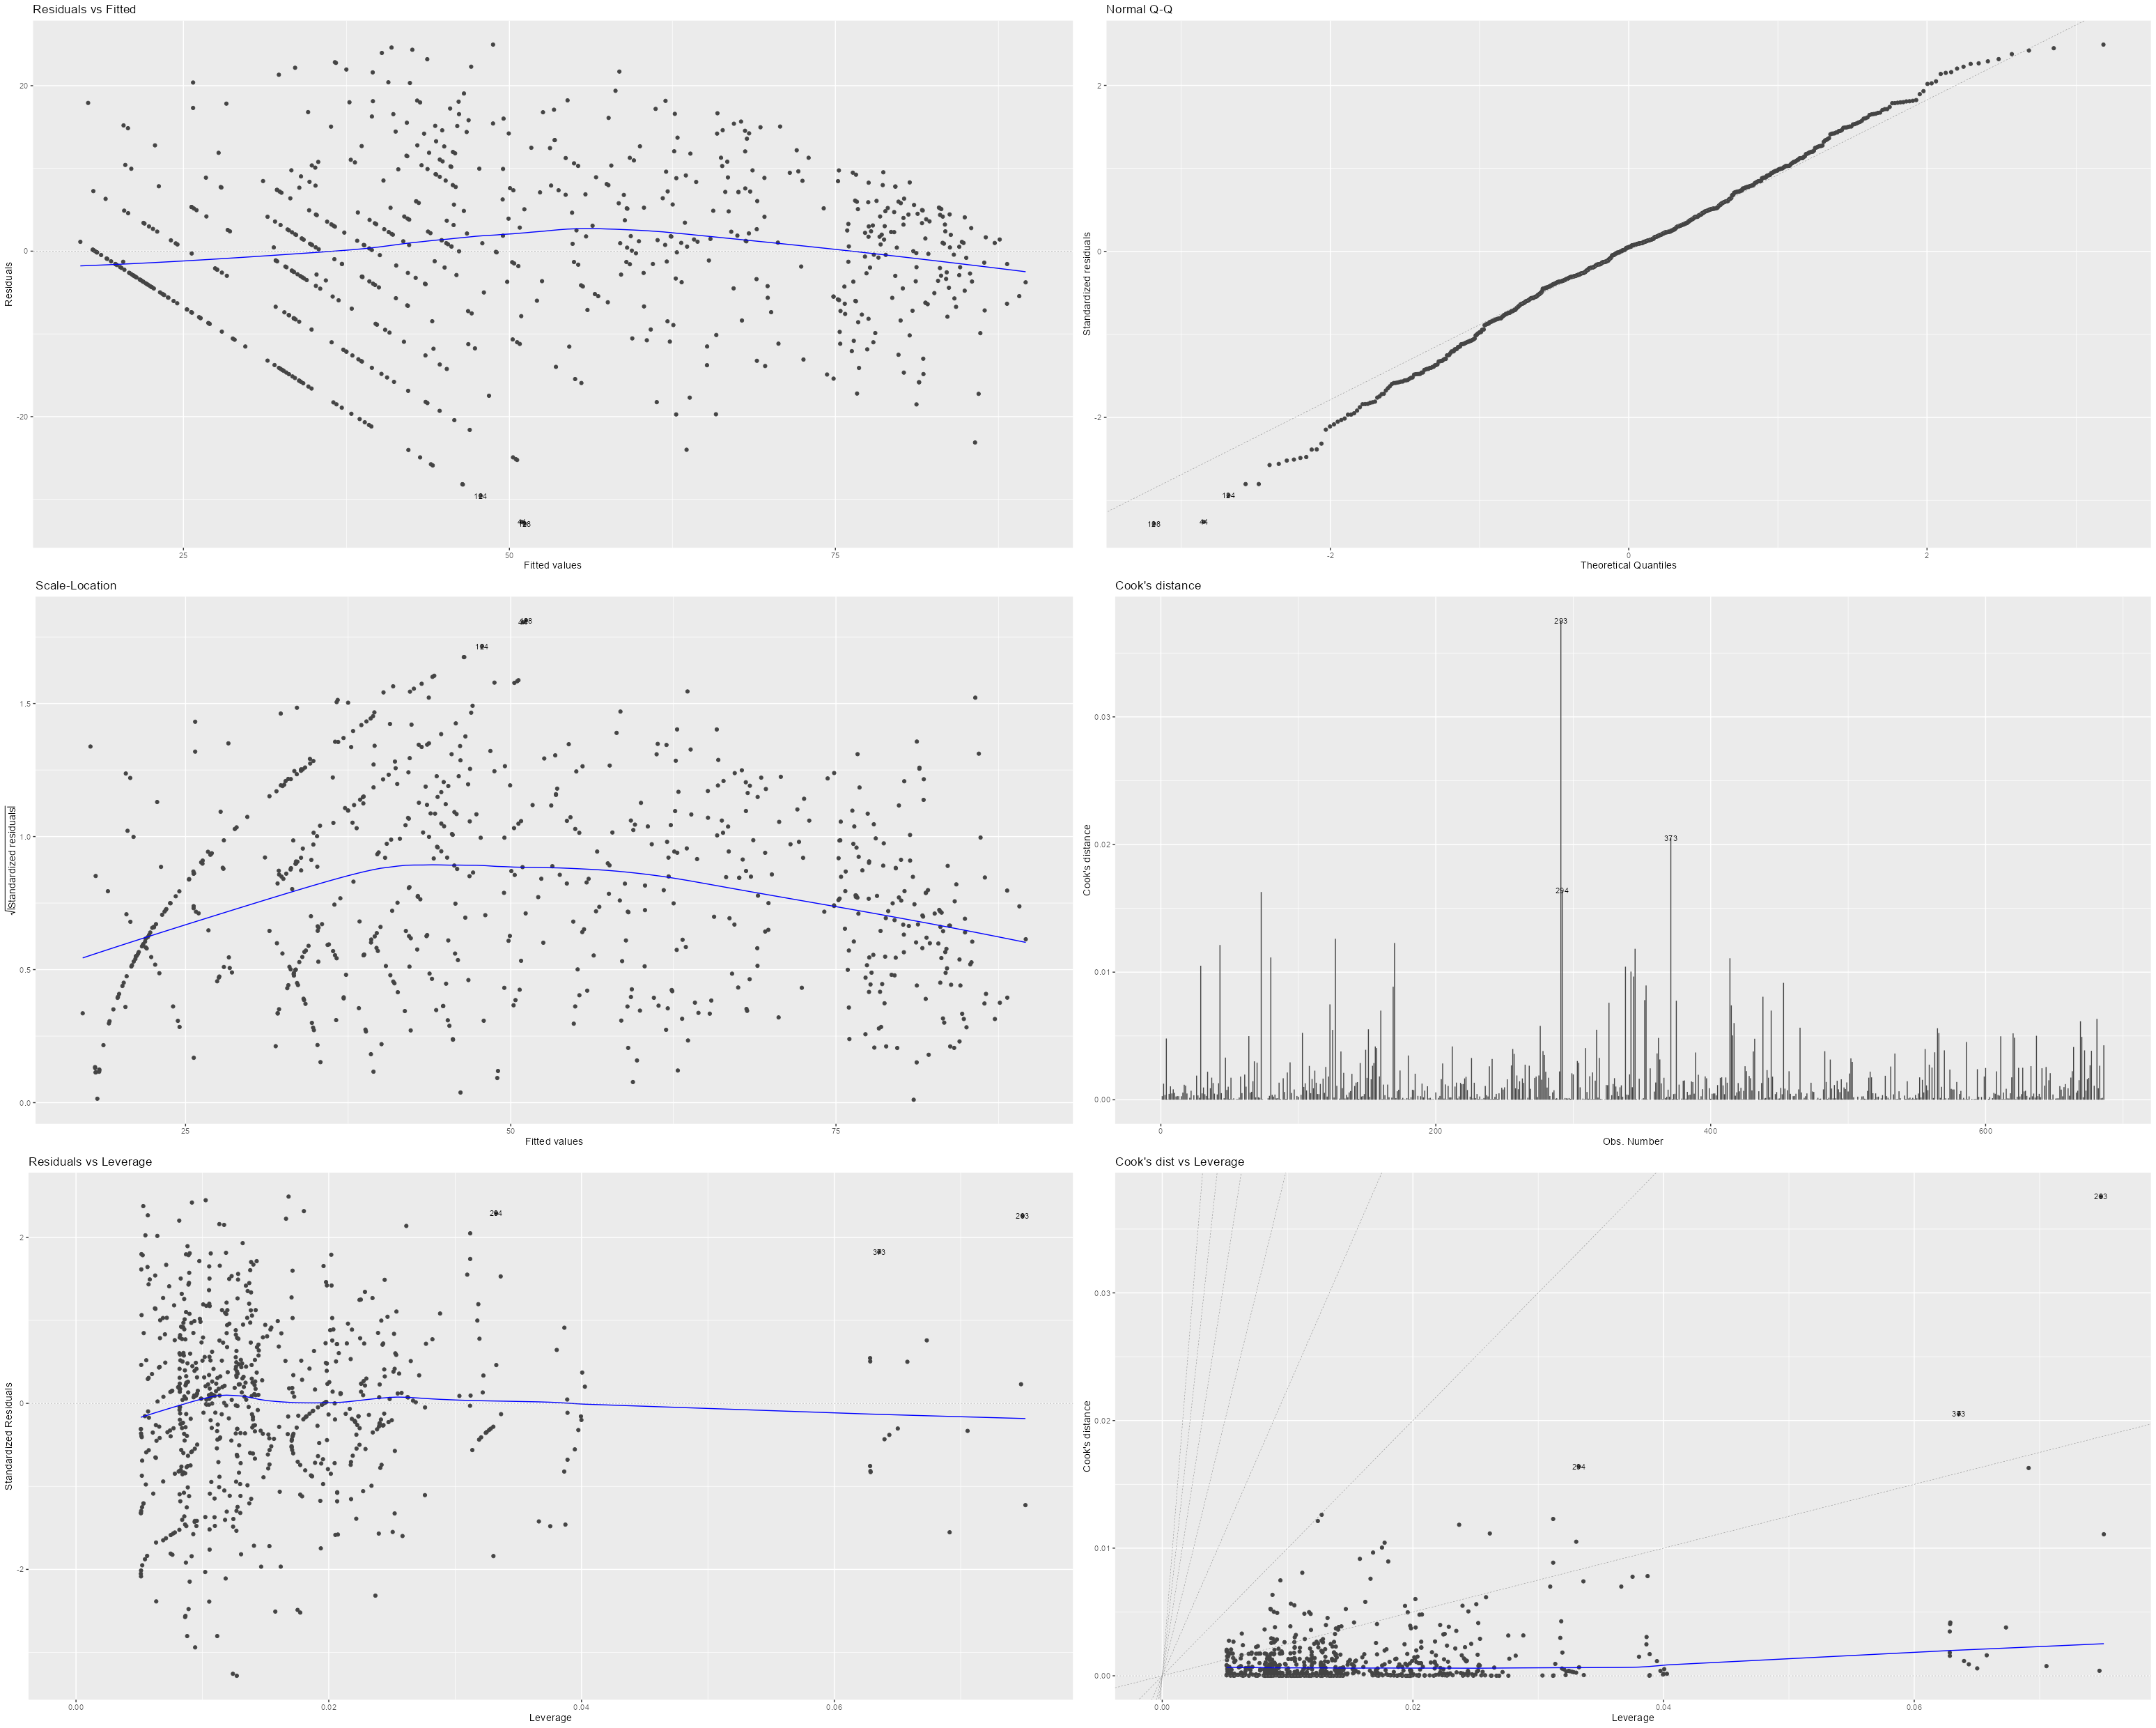
\includegraphics[width=.99\linewidth]{../01.Figures/anexo_1}}
  \\ \smallskip\noindent\scriptsize Fuente: Estimación propia con base en DESTA (2022) y Coppedge et al. (2022).
\end{figure*}
\pagebreak

\begin{table*}[h!]
  \centering
  \fontfamily{ppl}\selectfont
   \smallskip\noindent\small Anexo 2 \\ Pruebas de robustez \\~\\
  \begin{tabular}{l c c c}
    \toprule
     & Modelo V & Modelo Vb & Modelo Vc \\ \midrule
    \multirow{2}{*}{Nivel de democracia} & 0,196$^{\star\star\star}$ & 0,198$^{\star\star\star}$ & 0,342$^{\star\star}$ \\
    & {\scriptsize (0,020)} & {\scriptsize (0,021)} & {\scriptsize (0,114)} \\ 
    \multirow{2}{*}{Cap. Inversiones} & 17,285$^{\star\star\star}$ & 17,287$^{\star\star\star}$ & 17,598$^{\star\star\star}$ \\
    & {\scriptsize (1,001)} & {\scriptsize (1,001)} & {\scriptsize (1,013)} \\
    \multirow{2}{*}{Cap. Prop. Intelectual} & 13,277$^{\star\star\star}$ & 13,269$^{\star\star\star}$ & 13,357$^{\star\star\star}$ \\
    & {\scriptsize (1,077)} & {\scriptsize (1,078)} & {\scriptsize (1,081)}\\
    \multirow{2}{*}{Período 1961--1970} & 0,030 & -0,067 & 8,077 \\
    & {\scriptsize (3,083)} & {\scriptsize (3,095)} & {\scriptsize (5,986)} \\
    \multirow{2}{*}{Período 1971--1980} & 0,388 & 0,276 & 6,966 \\
    & {\scriptsize (2,915)} & {\scriptsize (2,931)} & {\scriptsize (5,667)} \\
    \multirow{2}{*}{Período  1981--1990} & -2,892 & -2,900 & 1,723 \\
    & {\scriptsize (2,851)} & {\scriptsize (2,853)} & {\scriptsize (5,490)} \\
    \multirow{2}{*}{Período 1991--2000} & 11,043$^{\star\star\star}$ & 11,021$^{\star\star\star}$  & 14,065$^{\star\star}$ \\
    & {\scriptsize (2,629)} & {\scriptsize (2,631)} & {\scriptsize (5,150)} \\ 
    \multirow{2}{*}{Período  2001--2010} & 17,802$^{\star\star\star}$ & 17,756$^{\star\star\star}$ & 26,51$^{\star\star\star}$ \\
    & {\scriptsize (2,685)} & {\scriptsize (2,690)} & {\scriptsize (5,31)} \\ 
    \multirow{2}{*}{Período 2010--2020} & 20,239$^{\star\star\star}$ & 20,169$^{\star\star\star}$ & 28,907$^{\star\star\star}$ \\
    & {\scriptsize (2,879)} & {\scriptsize (2,886)} & {\scriptsize (6,664)}\\
    \multirow{2}{*}{Acuerdo UE} & 4,807$^{\star\star\star}$ & 6,693 & 4,727$^{\star\star\star}$ \\
    & {\scriptsize (1,258)} & {\scriptsize (4,951)} & {\scriptsize (1,283)}\\
    \multirow{2}{*}{Nvl. democracia $\times$ Acuerdo UE} & & -0,030 & \\
    & & {\scriptsize (0,077)} & \\
    \multirow{2}{*}{Nvl. democracia $\times$ Período 1961--1970} & & & -0,218 \\
    & & & {\scriptsize (0,140)}\\
    \multirow{2}{*}{Democracia prom. $\times$ Período 1971--1980} & & & -0,174 \\
    & & & {\scriptsize (0,129)}\\
    \multirow{2}{*}{Nvl. democracia $\times$ Período 1981--1990} & & & -0,125 \\
    & & & {\scriptsize (0,127)}\\
    \multirow{2}{*}{Nvl. democracia $\times$ Período 1991--2000} & & & -0,100 \\
    & & & {\scriptsize (0,117)}\\
    \multirow{2}{*}{Nvl. democracia $\times$ Período 2001--2010} & & & -0,216 \\
    & & & {\scriptsize (0,121)}\\
    \multirow{2}{*}{Democracia prom. $\times$ Período 2010--2020} & & & -0,209 \\
    & & & {\scriptsize (0,137)}\\
    \multirow{2}{*}{Constante} & 19,028$^{\star\star\star}$ & 18,982$^{\star\star\star}$ & 13,585$^{\star\star}$  \\
    & {\scriptsize (2,628)} & {\scriptsize (2,632)} & {\scriptsize (4,904)} \\ \midrule
    $N$ & 686 & 686 & 686 \\ \midrule
    $R^2$ & 0,800 & 0,800 & 0,803 \\
    Adj. $R^2$ & 0,797 & 0,797 & 0,798 \\ \bottomrule
  \end{tabular}
  \\~\\ \smallskip\noindent\scriptsize $\star$ $p \leq 0,05$ | $\star\star$ $p \leq 0,01$ | $\star\star\star$ $p \leq 0,001$  \\ Fuente: Estimación propia con base en DESTA (2022) y Coppedge et al. (2022)
\end{table*}
\pagebreak

%%%%%%%%%%%%%%%%%%%%%%%%%%%%%%%%%%%%%%%%%%%%%%%%%%

\vspace{8mm}
\section[Informe de revisión]{\LARGE \itshape Informe abierto de revisi\'on}

%%%%%%%%%%%%%%%%%%%%%%%%%%%%%%%%%%%%%%%%%%%%%%%%%%

\vspace{8mm}
{\noindent {\Large Carla Cisternas} \footnote{(PhD) Researcher, Department of  Latin American Studies, Faculty of Humanities, Leiden University. ORCID iD: \href{https://orcid.org/0000-0001-7948-6194}{\textcolor{blue}{0000-0001-7948-6194}}} \\
{\normalsize Leiden University} \\
\vspace{1mm}{\LARGE \Letter} \href{mailto:c.g.cisternas.guasch@hum.leidenuniv.nl }{\textcolor{blue}{\normalsize c.g.cisternas.guasch@hum.leidenuniv.nl }}}
\vspace{8mm}

\justify{\textcolor{red}{\lipsum[1]}}

\justify{\textcolor{red}{\lipsum[1]}}

\justify{\textcolor{red}{\lipsum[1]}}

%%%%%%%%%%%%%%%%%%%%%%%%%%%%%%%%%%%%%%%%%%%%%%%%%%

\section{{\normalfont CRediT -- Contributor Roles Taxonomy}}

%%%%%%%%%%%%%%%%%%%%%%%%%%%%%%%%%%%%%%%%%%%%%%%%%%

{\noindent {\bfseries Rodrigo Cuevas} (autor)}

{\noindent {\includegraphics[width=.085\linewidth]{../../badges/conceptualization} {\includegraphics[width=.085\linewidth]{../../badges/data_curation} {\includegraphics[width=.085\linewidth]{../../badges/formal_analysis} {\includegraphics[width=.085\linewidth]{../../badges/funding_acquisition} {\includegraphics[width=.085\linewidth]{../../badges/methodology} {\includegraphics[width=.085\linewidth]{../../badges/resources} {\includegraphics[width=.085\linewidth]{../../badges/computation} {\includegraphics[width=.085\linewidth]{../../badges/supervision} {\includegraphics[width=.085\linewidth]{../../badges/testing} {\includegraphics[width=.085\linewidth]{../../badges/data_visualization} {\includegraphics[width=.085\linewidth]{../../badges/writing_initial_draft}
{\includegraphics[width=.085\linewidth]{../../badges/writing_review}}\\

{\noindent {\bfseries Bastián González-Bustamante} (editor)}

{\noindent {\includegraphics[width=.085\linewidth]{../../badges/writing_review}}\\

{\noindent {\bfseries Jaquelin Morillo} (editora)}

{\noindent {\includegraphics[width=.085\linewidth]{../../badges/writing_review}}\\

{\noindent {\bfseries Carla Cisternas} (evaluadora)}

{\noindent {\includegraphics[width=.085\linewidth]{../../badges/writing_review}}\\

{\noindent {\bfseries Antonia Pérez} (asistente de investigación)}

{\noindent {\includegraphics[width=.085\linewidth]{../../badges/investigation}}

%%%%%%%%%%%%%%%%%%%%%%%%%%%%%%%%%%%%%%%%%%%%%%%%%%

\section{{\normalfont Historial de revisiones}}

%%%%%%%%%%%%%%%%%%%%%%%%%%%%%%%%%%%%%%%%%%%%%%%%%%

\vspace{-0.6cm}
\begin{table}[h!]
\begin{tabular}{@{}lll@{}}
{\small 1,0} & {\small 5 octubre 2022} & {\small Manuscrito original} \\[0.8mm]
{\small 2,0} & {\small 19 diciembre 2022} & {\small Manuscrito revisado} \\[0.8mm]
{\small 3,0} & {\small 31 diciembre 2022} & {\small Fecha de publicación} \\[0.8mm]
{\small 4,0$^\dagger$} & {\small 6 enero 2023} & {\small Correcciones menores} \\[0.8mm]
{\small 5,0$^\dagger$} & {\small TBC} & {\small Correcciones menores} \\
\end{tabular}
\end{table}
\vspace{0.3cm}
{\noindent \footnotesize {\normalsize \faCloudDownload} Descargar la versión más reciente desde SocArXiv ({\scriptsize DOI:} \href{https://doi.org/10.31235/osf.io/y4fxw}{\textcolor{blue}{10.31235/osf.io/y4fxw}}).}
{\noindent \scriptsize {\normalsize $^\dagger$} versión disponible en SocArXiv.}

\end{document}
